\subsection{Towards robust boosted jet tagging}
\label{sec:searchII:intro}
When we first studied W-tagging at 13 \TeV in context with the analysis of the 2015 dataset, Section~\ref{sec:searchI:wtagging}, two interesting correlations were observed:

\bigskip
1) A strong dependence of the AK8 CHS softdrop ($\beta = 0$) jet mass on jet \PT and

2) a strong dependence of the AK8 CHS $\tau_{21}$ cut efficiency on pileup.
\bigskip

The reason we studied the softdrop algorithm as an alternative to pruning in 2015 was, besides the possibility it would result in a higher signal efficiency, that we knew it had certain favorable qualities compared to other groomers: Softdrop removes all sensitivity to the soft divergences of QCD, by removing all soft emission, more specifically the non-global logarithmic terms (NGLs) in the jet mass~\cite{Dasgupta:2013ihk}. These arise from constellations where, for instance, a soft gluon is radiated into the jet cone, as illustrated in Figure~\ref{fig:searchII:ngls}. 
\begin{figure}[h!]
\centering
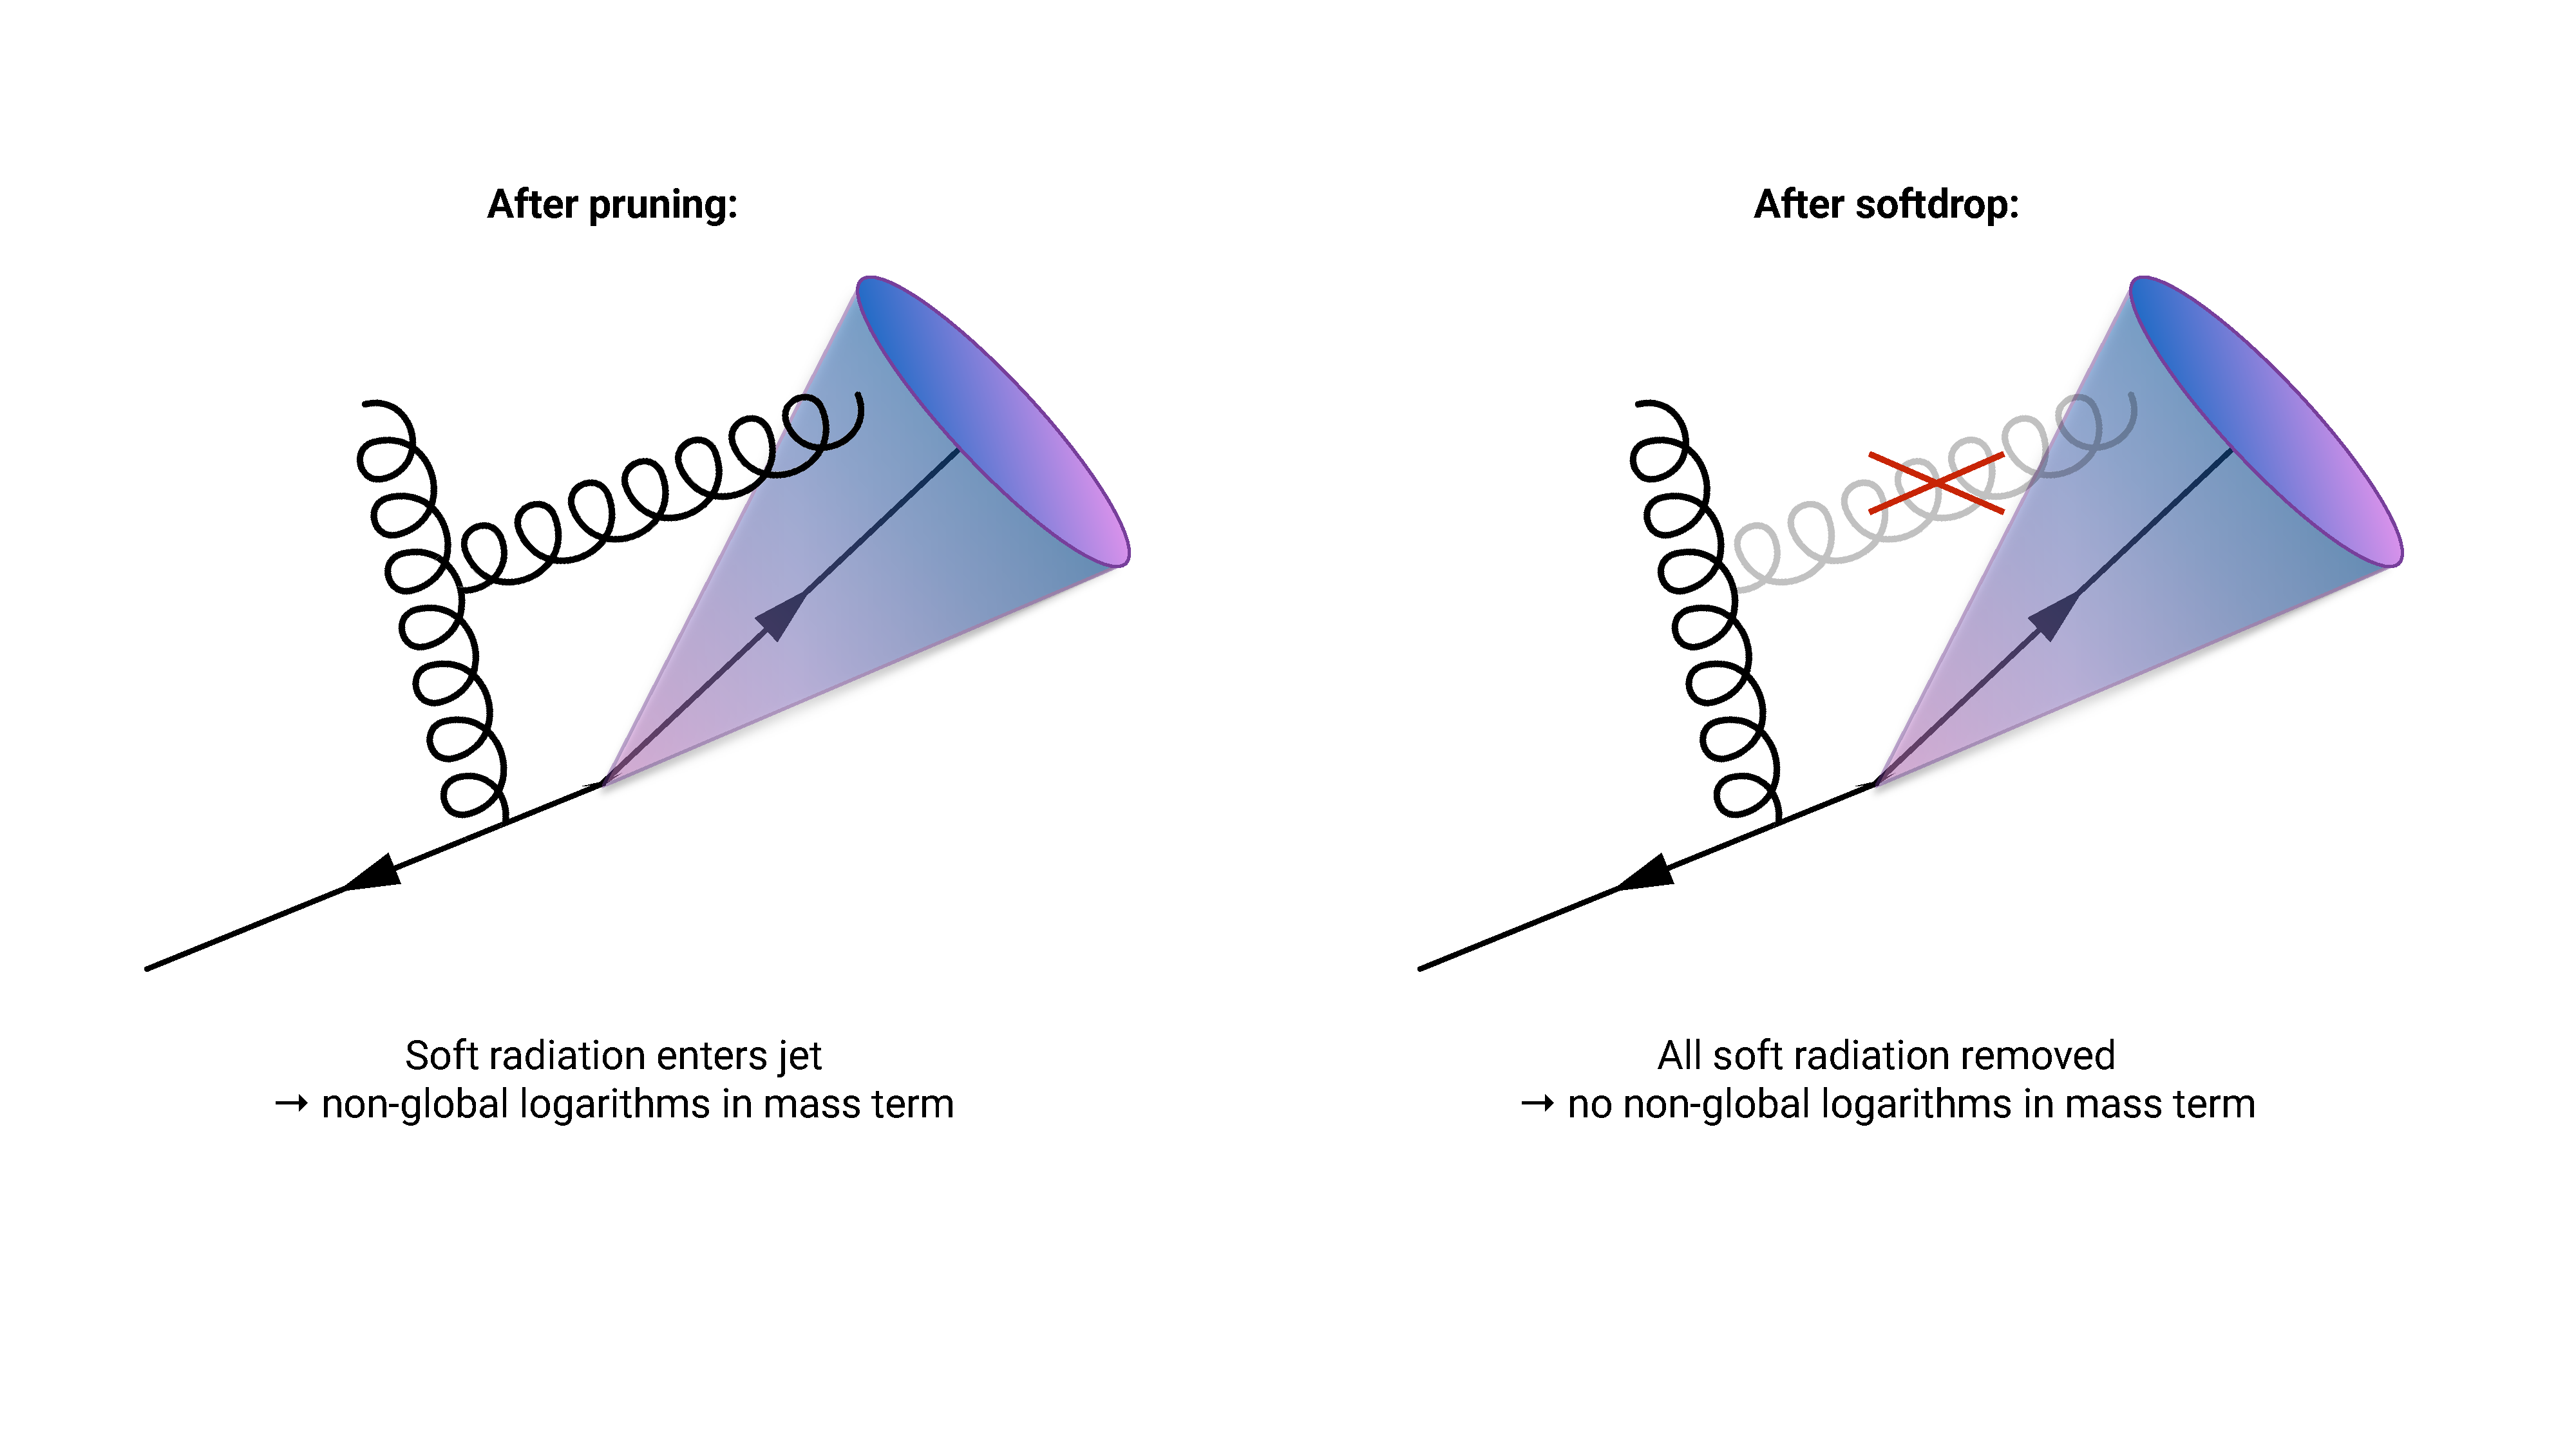
\includegraphics[width=0.69\textwidth]{figures/analysis/search2/misc/ngls.pdf}
\caption{The pruning algorithm does not remove all soft emission and therefore has non-global logarithmic terms in the jet mass. Softdrop ($\beta = 0$) completely removes soft emissions and is therefore free of non-global logarithms.}
\label{fig:searchII:ngls}
\end{figure}
The consequence of this is that you can calculate the softdrop jet mass to way higher precision than what is possible for other grooming algorithms or for the plain jet mass (NGLs are the main reason a full resummation of the plain jet mass beyond NLL (considering e.g multiple-emission effects) accuracy does not exist). Despite this not being a precision measurement analysis, we had theoretically well-motivated reasons for wanting the baseline CMS V-tagger to be softdrop-based. However, despite being less sensitive to soft radiation for QCD jets, signal jets groomed with softdrop were found to be far more sensitive to the underlying event than pruned jets~\cite{Dasgupta:2015yua}. Figure~\ref{fig:searchII:ue} shows the signal efficiency for pruning (left) and softdrop (right) as a function of jet transverse momenta when including FSR only, FSR+ISR, hadronization and hadronization + underlying event.
\begin{figure}[h!]
\centering
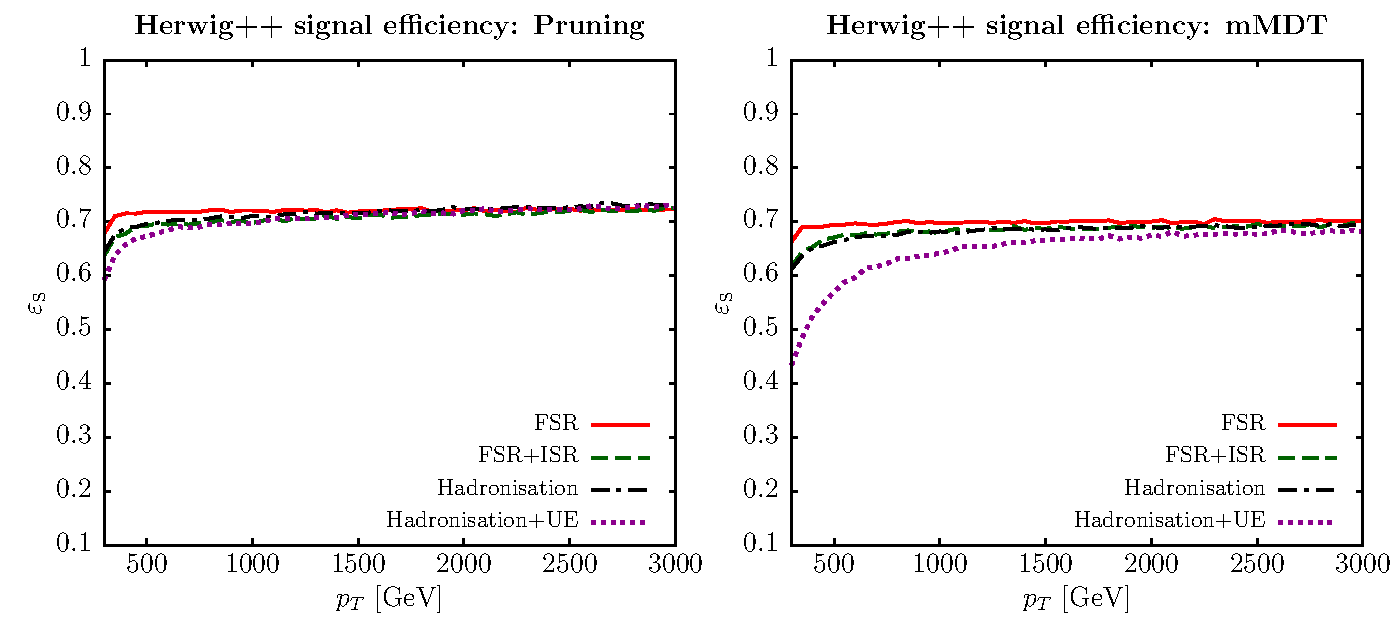
\includegraphics[width=0.79\textwidth]{figures/analysis/search2/misc/pruningvssd_ue.pdf}
\caption{The signal efficiency for pruning (left) and softdrop (right) as a function of jet \PT when adding FSR, ISR, hadronization and UE. THe UE has a severe impact on the softdrop efficiency for signal jets~\cite{Dasgupta:2015yua}. }
\label{fig:searchII:ue}
\end{figure}
On parton level, as well as after hadronization, the two algorithms perform very similar as a function of \PT. However, once UE contamination is added, the softdrop tagging efficiency is severely affected. This can be explained by the larger effective radius considered by the softdrop algorithm ( $\propto \mV/\PT \sqrt{z_{cut}(1-z_{cut})}$ ) in comparison to pruning ( $\propto \mV/\PT$ ). This observation corresponds very well with the shift in jet mass we observed for softdrop as a function of \PT in Section~\ref{sec:searchI:wtagging}: As the jet \PT decreases the softdrop effective radius increases and the jet mass mean shifts to higher values, due to absorbing more background radiation. If softdrop would be our new default tagger, a better rejection of pileup and UE contamination would be needed. In parallel to the ongoing theoretical work on groomers, a novel pileup removal algorithm had been proposed: Pileup per particle identification (PUPPI)~\cite{Bertolini2014}. Described in detail in Section~\ref{subsub:objreco:puppi}, PUPPI considers not only charged pileup but rather reweights each particle in the jet with its probability of arising from pileup. PUPPI had proven it self far superior to the current CHS algorithm in terms of jet observables for large radius jets, and therefore seemed like the obvious choice to address both issues listed above: The sensitivity of softdrop regarding UE contamination and the strong pileup dependence of $\tau_{21}$. The focus of Search II would therefore be on the commissioning of a novel W-tagger. There are interesting changes and inclusions in the analysis strategy as well: The inclusion of a $\PZpr \rightarrow \WW$ signal hypothesis and the addition of a completely new analysis, the single V-tag analysis.

\subsection{Analysis strategy}
The analysis strategy for this search is conceptually the same as for Search I. In addition, we'll take advantage of the n-subjettiness categorization and do an additional analysis in parallel: A search for excited quark resonances $\rm{q^*}$~\cite{Bauer1987,PhysRevD.42.815} decaying to qW or qZ.
We call this the single V-tag analysis, and the analysis selection only differs in that one jet is not required to pass the V-tag selection (groomed mass and n-subjettiness). The \VV analysis is hereby referred to as the double V-tag analysis. The difference between the two analyses is illustrated in Figure~\ref{fig:searchII:svsd}. 
\begin{figure}[h!]
\centering
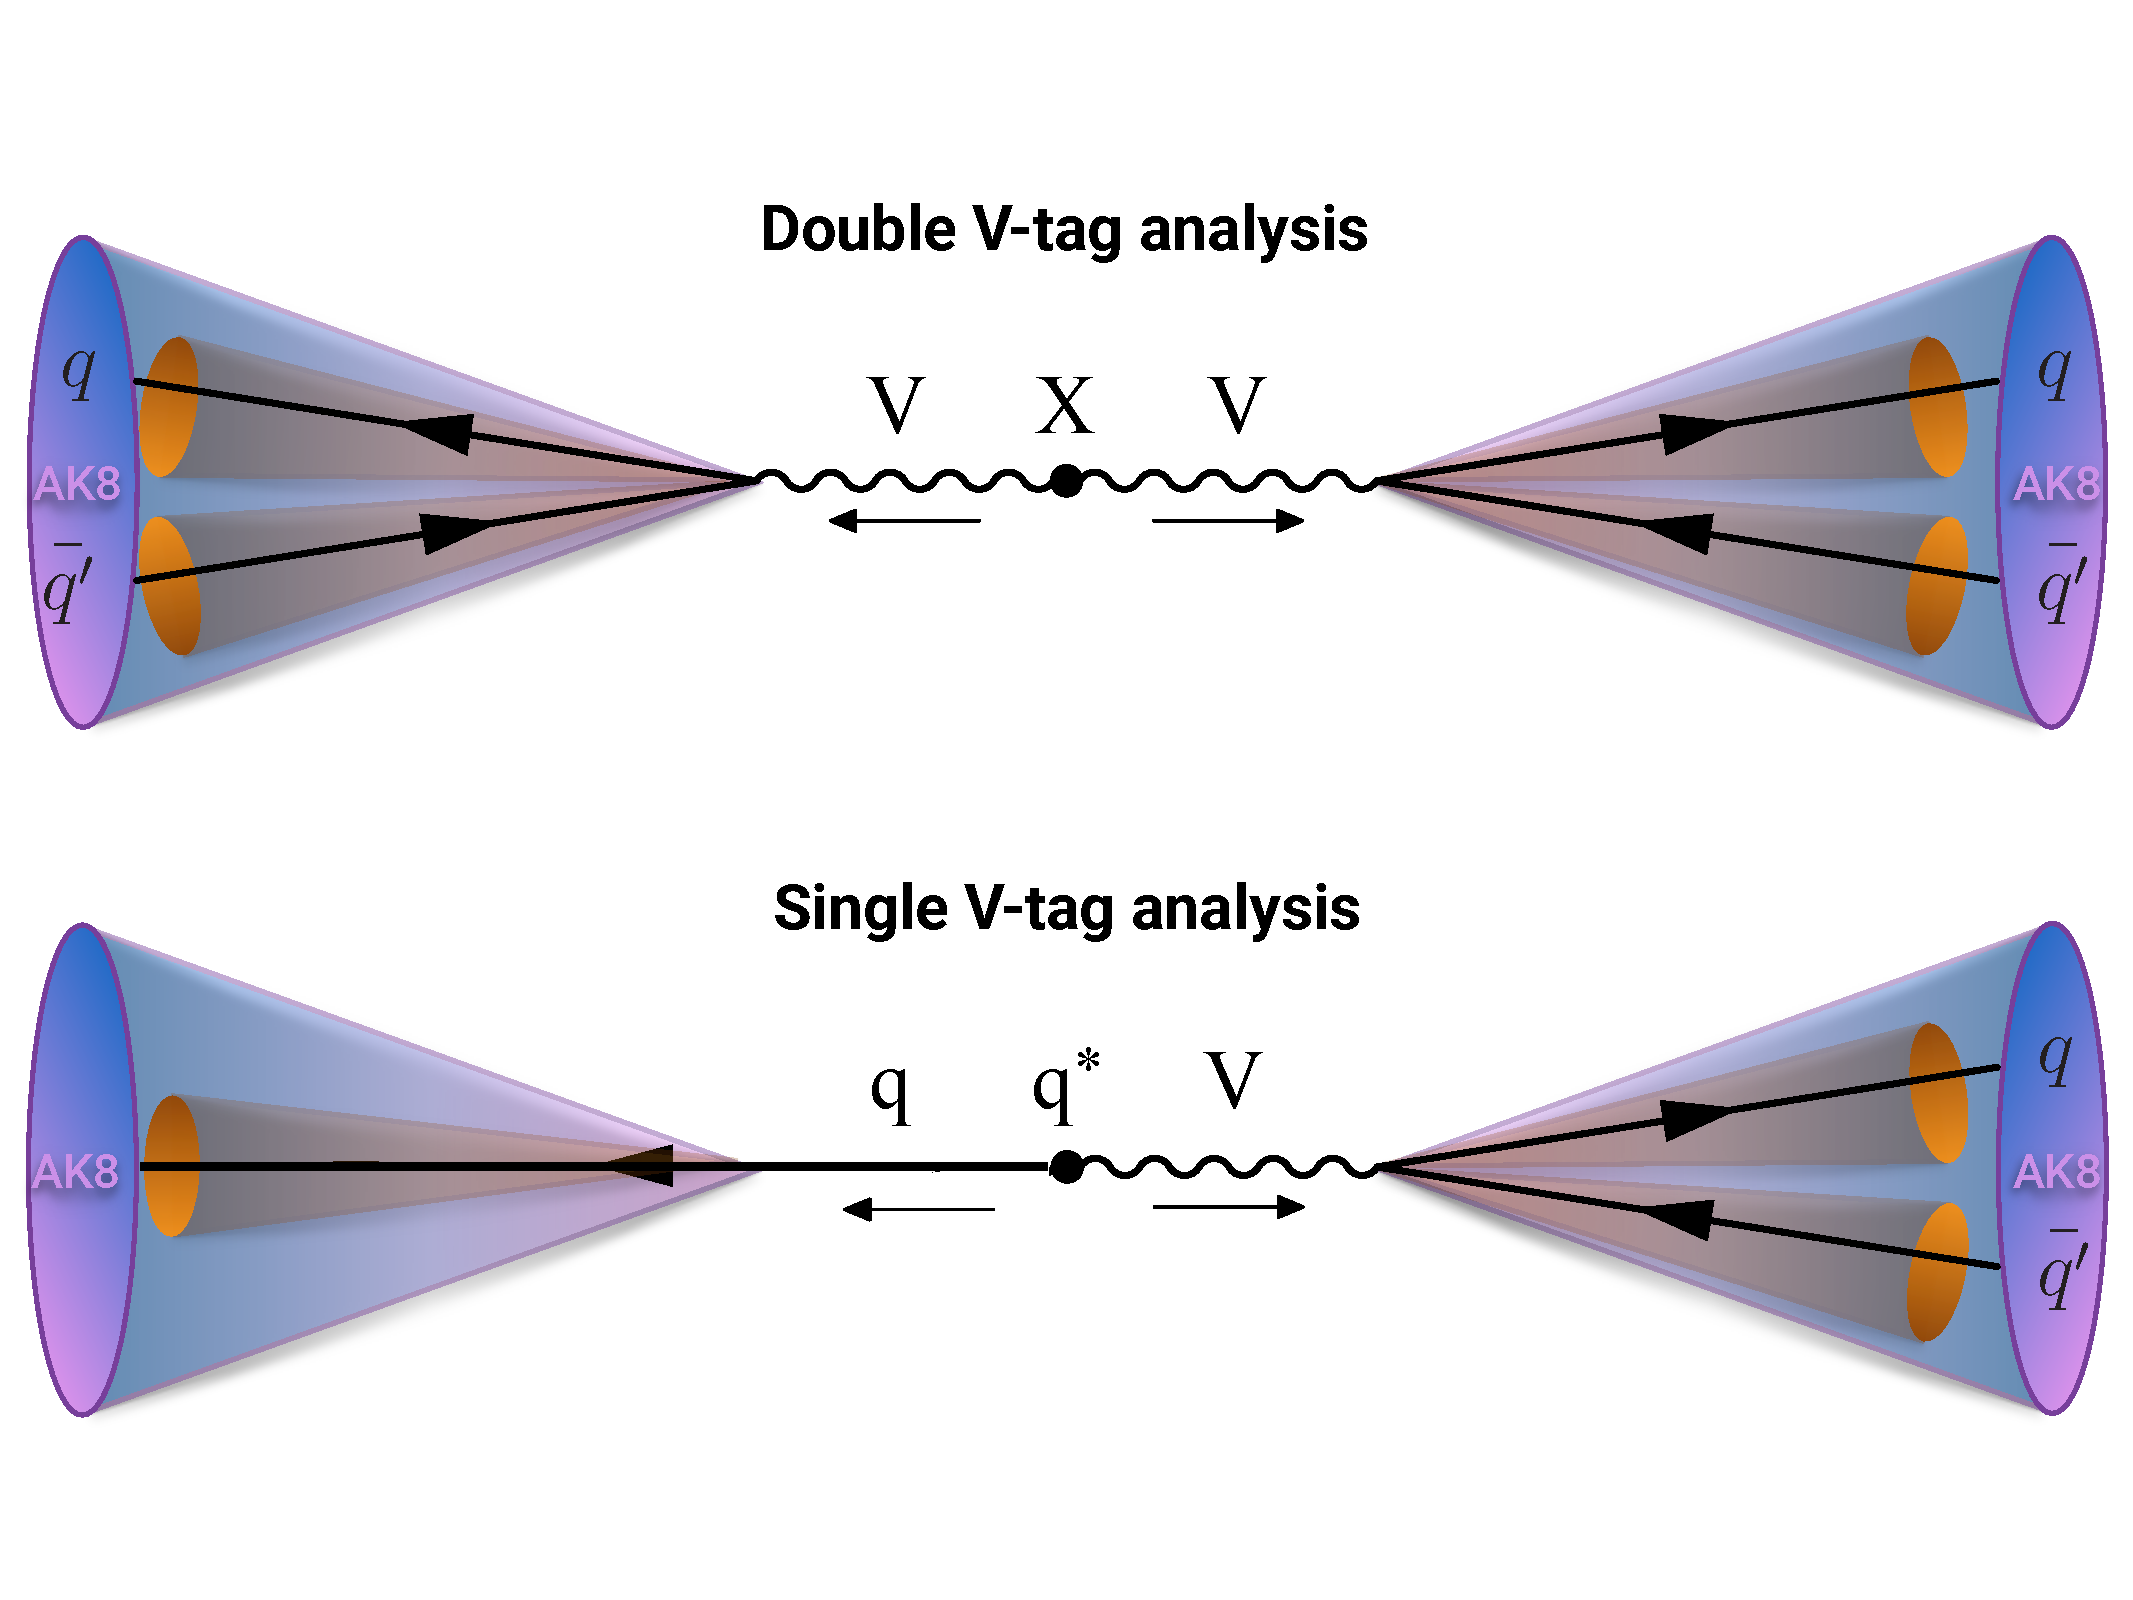
\includegraphics[height=6.5cm]{figures/analysis/search2/misc/singlevsdoubletag.pdf}
\caption{The double (top) and single (bottom) W/Z-tag analysis.}
\label{fig:searchII:svsd}
\end{figure}
In addition, limits are set on a $\PZpr \rightarrow \WW$ signal hypothesis in the double V-tag analysis, another 13 \TeV first.\newline
This analysis was published in two steps: An early Physics Analysis Summary (PAS) based on 12.9 \fbinv of 2016 data~\cite{CMS-PAS-B2G-16-021}, describing the new  PUPPI+softdrop based V-tagger as well as the single V-tag analysis, and a second analysis topping up with the full 2016 data~\cite{PhysRevD.97.072006}. The commissioning of the new \PW\PZ-tagger has also been documented in a jet performance Physics Analysis Summary~\cite{CMS-PAS-JME-16-003}. As the new V-tagger was developed and commissioned in the context of the early analysis, which was also were the single V-tag analysis was first published with 13 \TeV data, the main emphasis will be on the work presented in CMS-PAS-B2G-16-021~\cite{CMS-PAS-B2G-16-021}. The second part of the results chapter, Section~\ref{sec:searchII:brg17001res}, includes the results obtained using the full 2016 dataset of 35.9 \fbinv.

\subsection{Data and simulated samples}
\label{sec:searchII:samples}
As mentioned above, the analysis of the 2016 dataset was done in two steps: One analysis based on 12.9 \fbinv of early 2016 data, describing the new W-tagger and single V-tag category, and a second paper topping up with the full 2016 dataset, corresponding to 35.9 \fbinv.\par
The \BulkG and HVT signal samples are modeled in precisely the same way as in 2015. For the single V-tag $\textrm{q}^*$ samples, we simulate unpolarized boson with a compositeness scale $\Lambda$ set equal to the resonance mass. These are generated to leading order using \PYTHIA version 8.212~\cite{Sjostrand:2007gs}. \par
The background Standard Model processes; QCD, W+jets and Z+jets are all simulated to leading order. V+jets is simulated with \amcatnlo~\cite{Alwall:2014hca,Alwall:2007fs}, while three different combinations of matrix element and shower generators is used for QCD as these predictions are known to differ: \PYTHIA only, the leading order mode of \amcatnlo{} matched with \PYTHIA, and \HERWIG{++}~2.7.1~\cite{Bahr:2008pv} with tune CUETHS1~\cite{Khachatryan:2015pea}.

\subsection{Event selection}
\subsubsection{Triggering}
The triggers used in this analysis are the same ones as in 2015 (see Section~\ref{sec:searchI:trigger}), however, due to the new single V-tag analysis, the trigger turn-ons have this time been re-evaluated separately requiring either one or two jets to have an offline softdrop jet mass above 65 \GeV.
\par Figure~\ref{fig:searchII:trigger-fits} shows the trigger turn-on curves as a function of dijet invariant mass for jets passing one of the three inclusive triggers only, one of the grooming triggers only and when combining all of them. The turn-on curves are shown for all jet pairs passing loose selections as described in Section \ref{sec:searchI:preselection}. Zero, one or two of the two jets is further required to have a softdrop mass larger than 65 GeV.

\begin{figure}[h!]
\centering
% 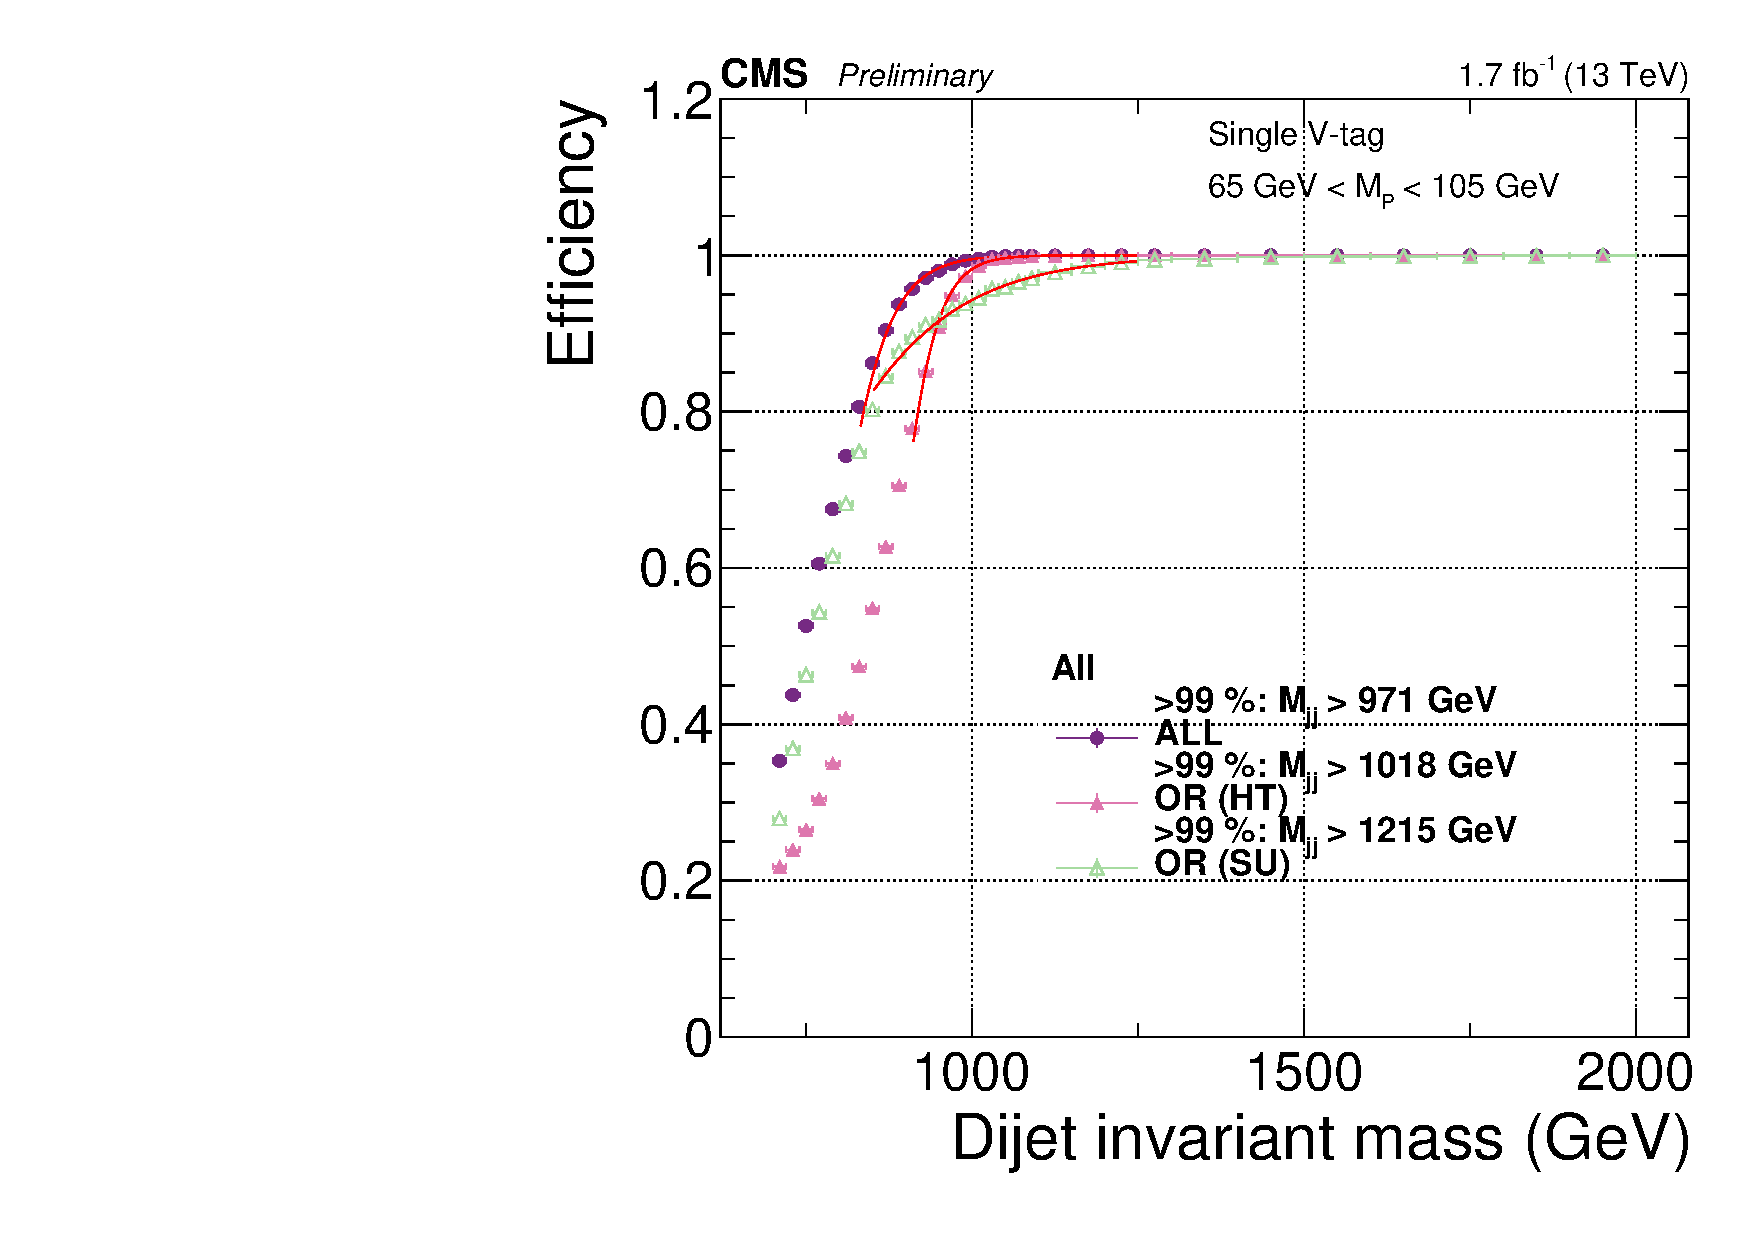
\includegraphics[width=0.4\textwidth]{figures/analysis/search2/AN-16-398/plots/trigger/triggereffMjj-ALL_SingleTag_runAll.pdf}
% 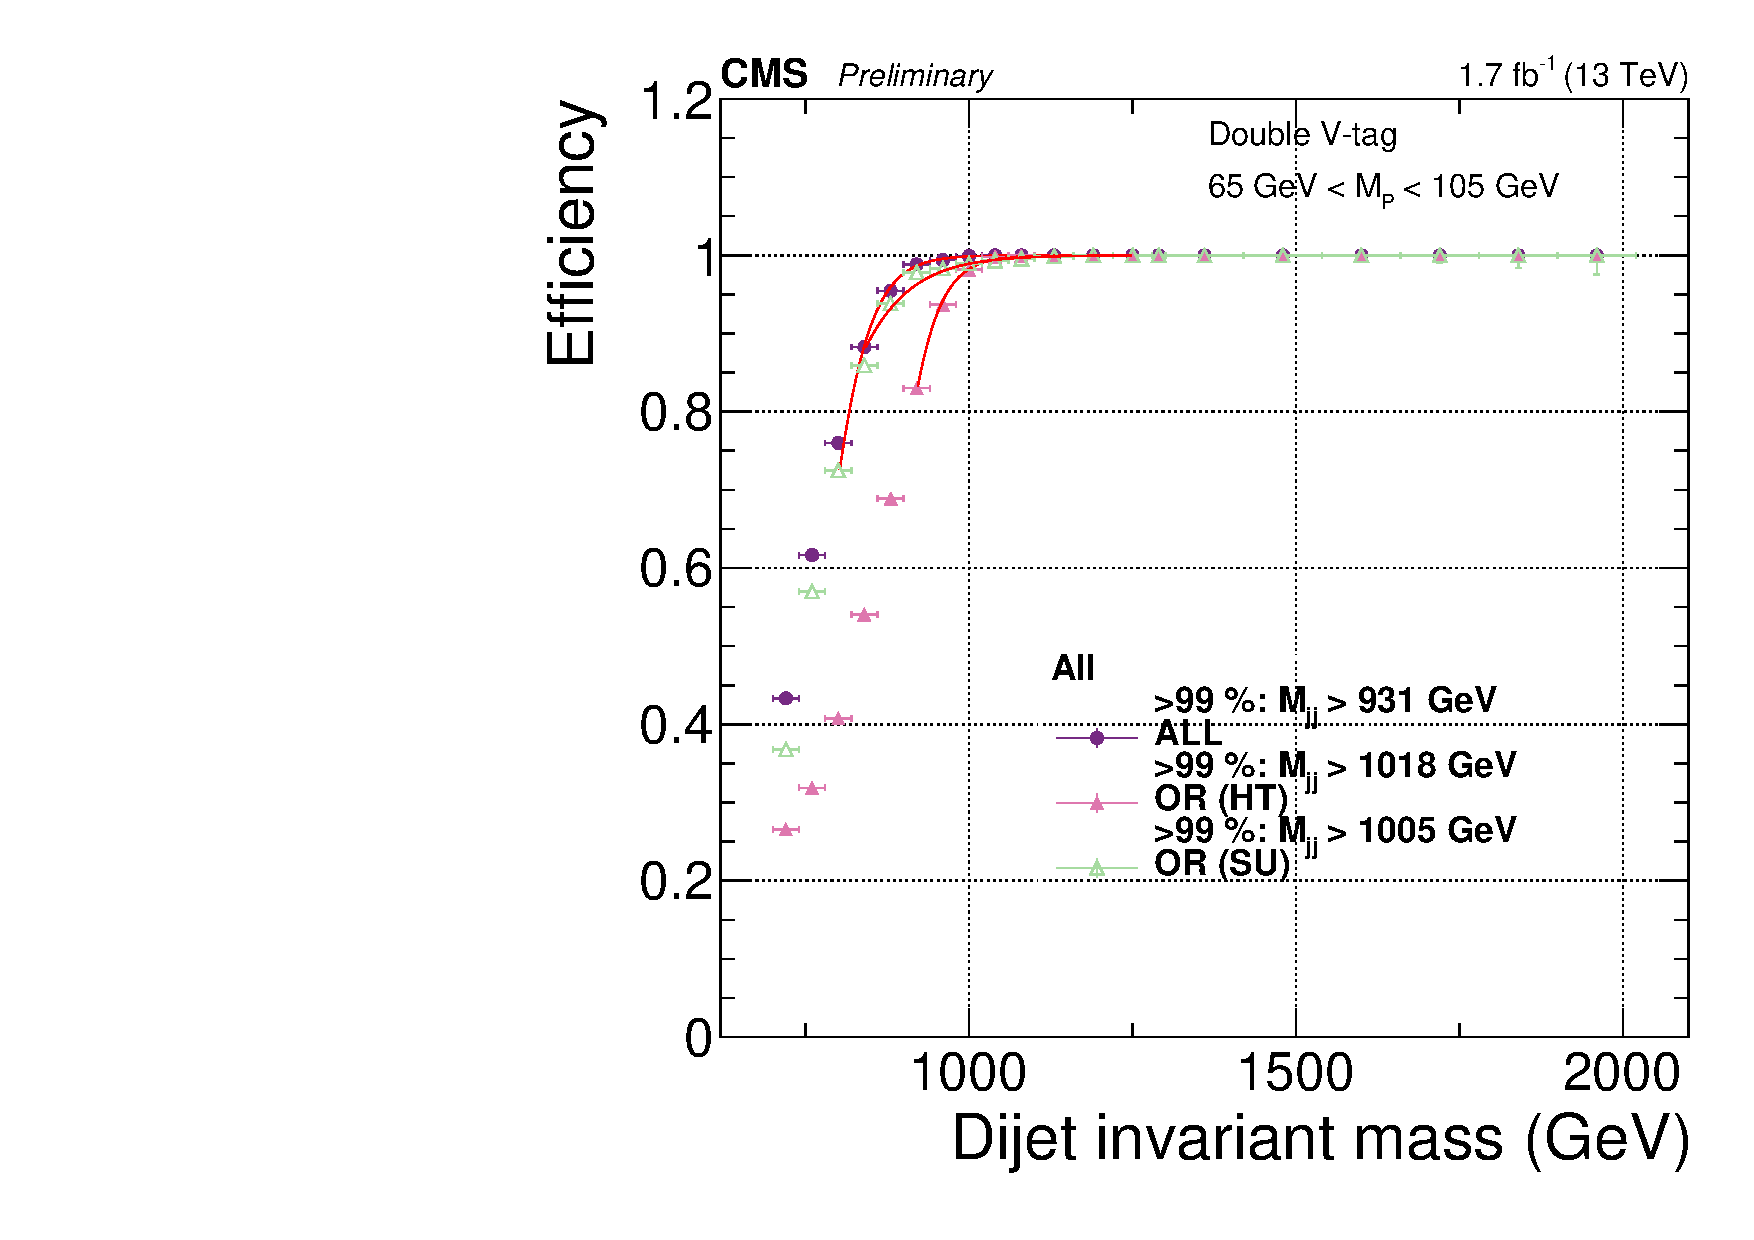
\includegraphics[width=0.4\textwidth]{figures/analysis/search2/AN-16-398/plots/trigger/triggereffMjj-ALL_DoubleTag_runAll.pdf}
% 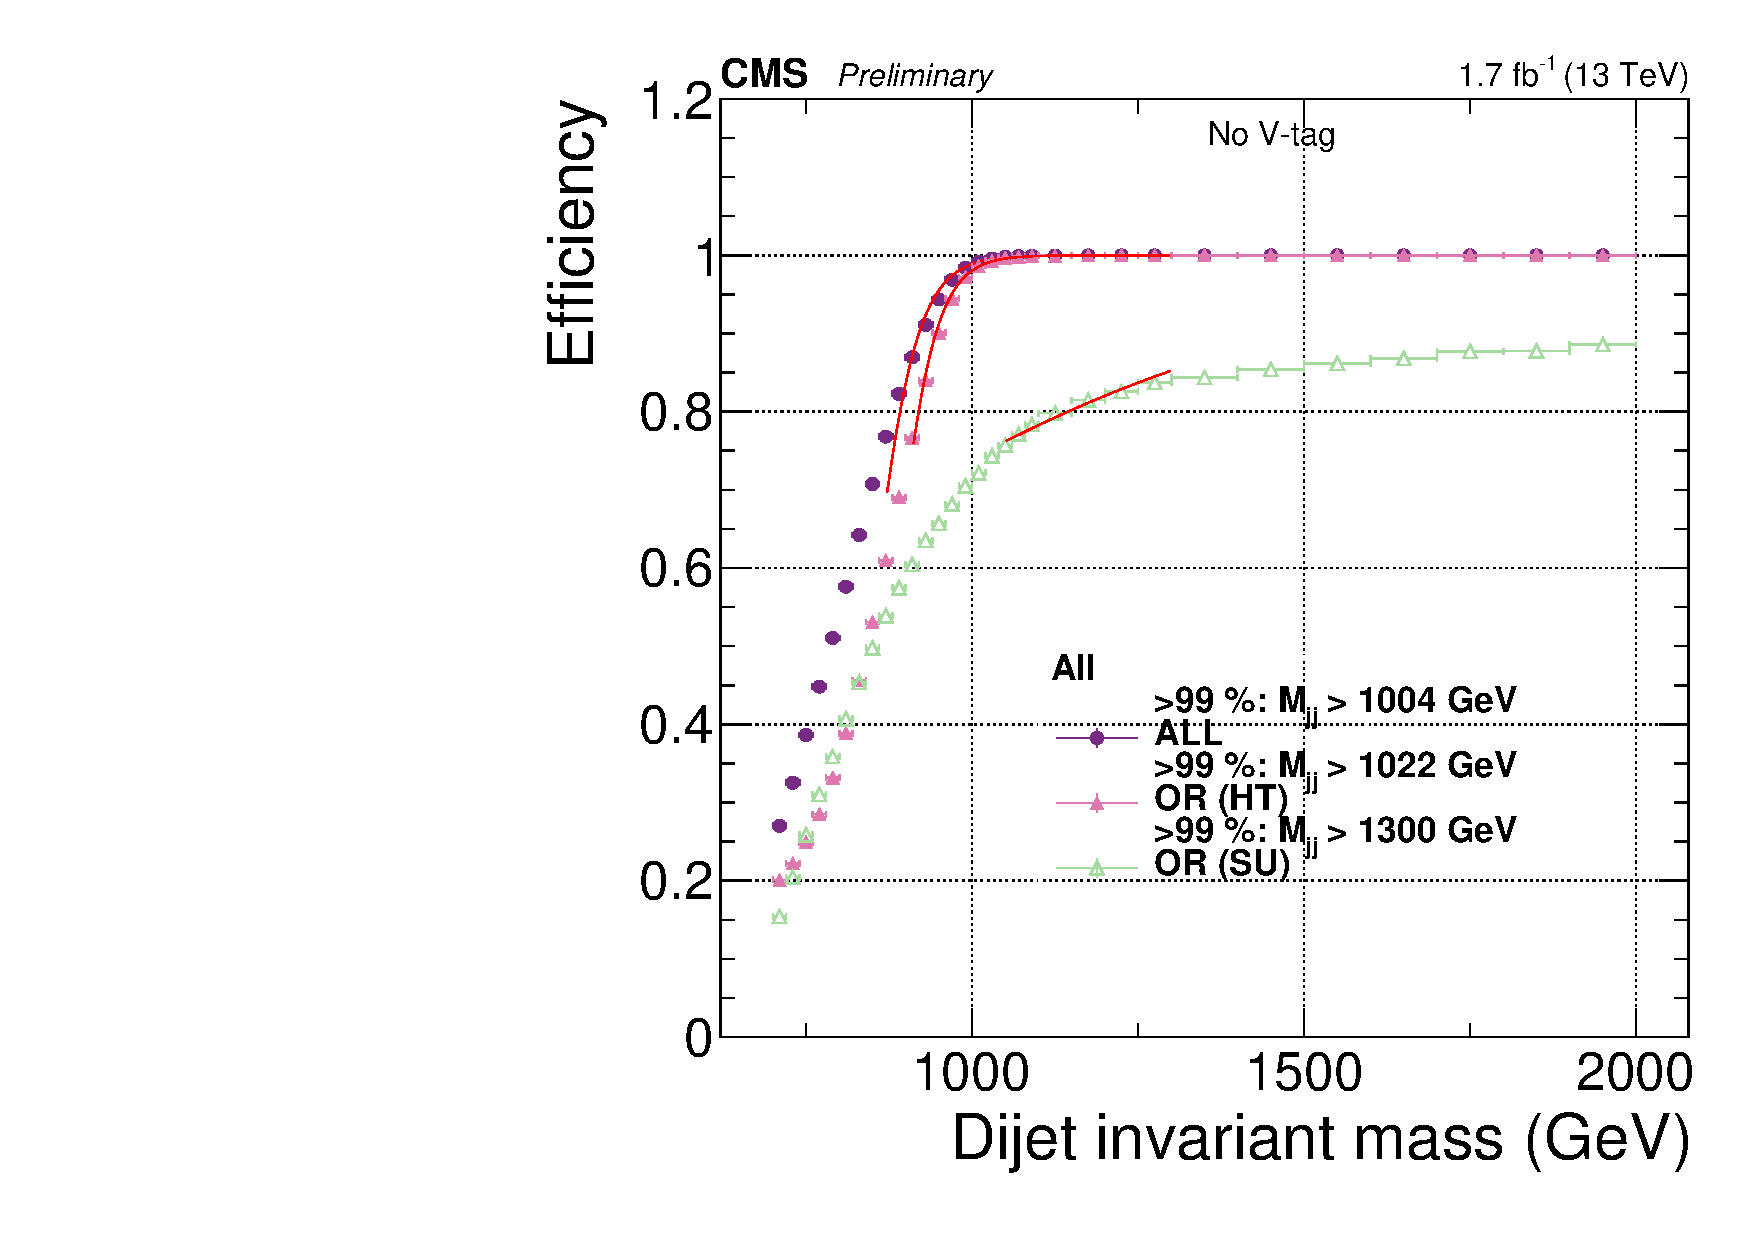
\includegraphics[width=0.4\textwidth]{figures/analysis/search2/AN-16-398/plots/trigger/triggereffMjj-ALL_noTag_runAll.pdf}
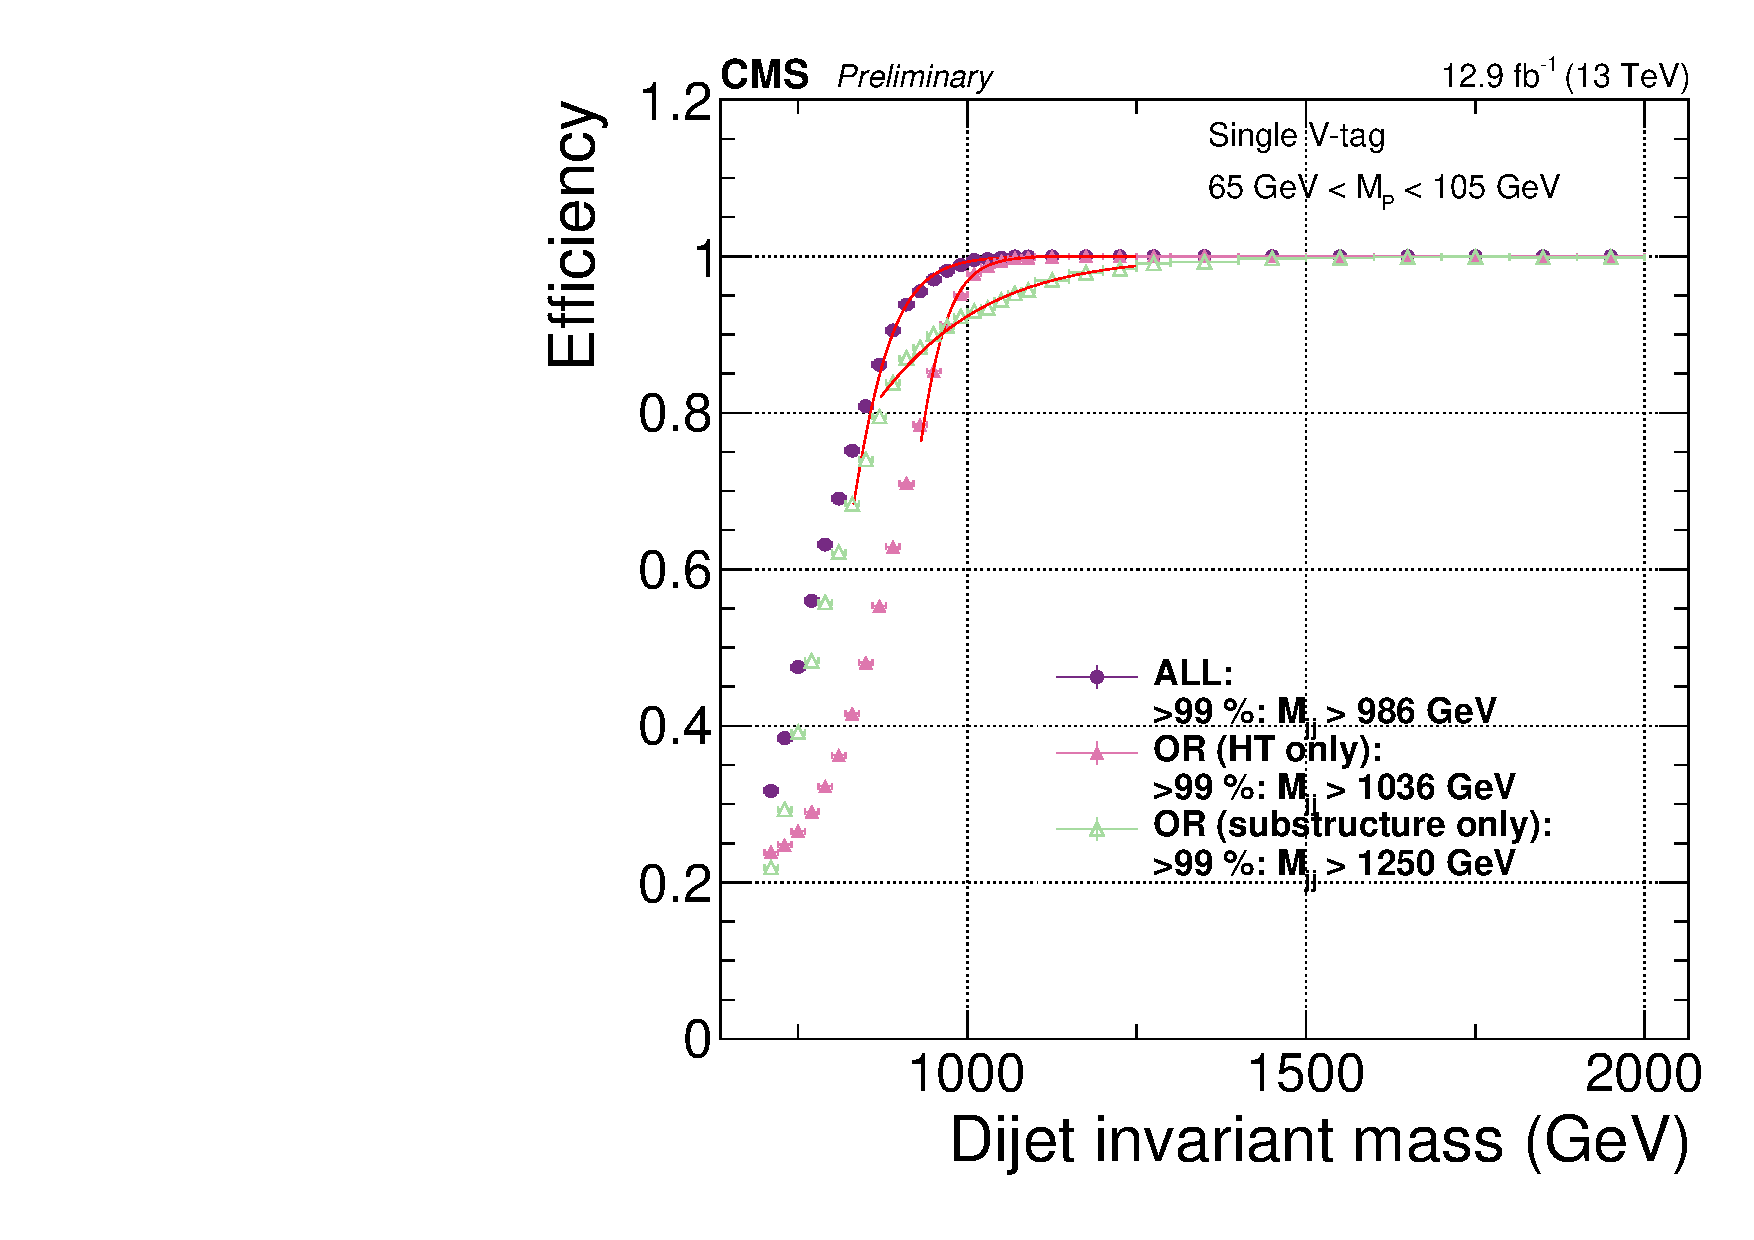
\includegraphics[width=0.49\textwidth]{figures/analysis/search2/AN-16-235/plots/triggereffMjj-ALL_SingleTag.pdf}
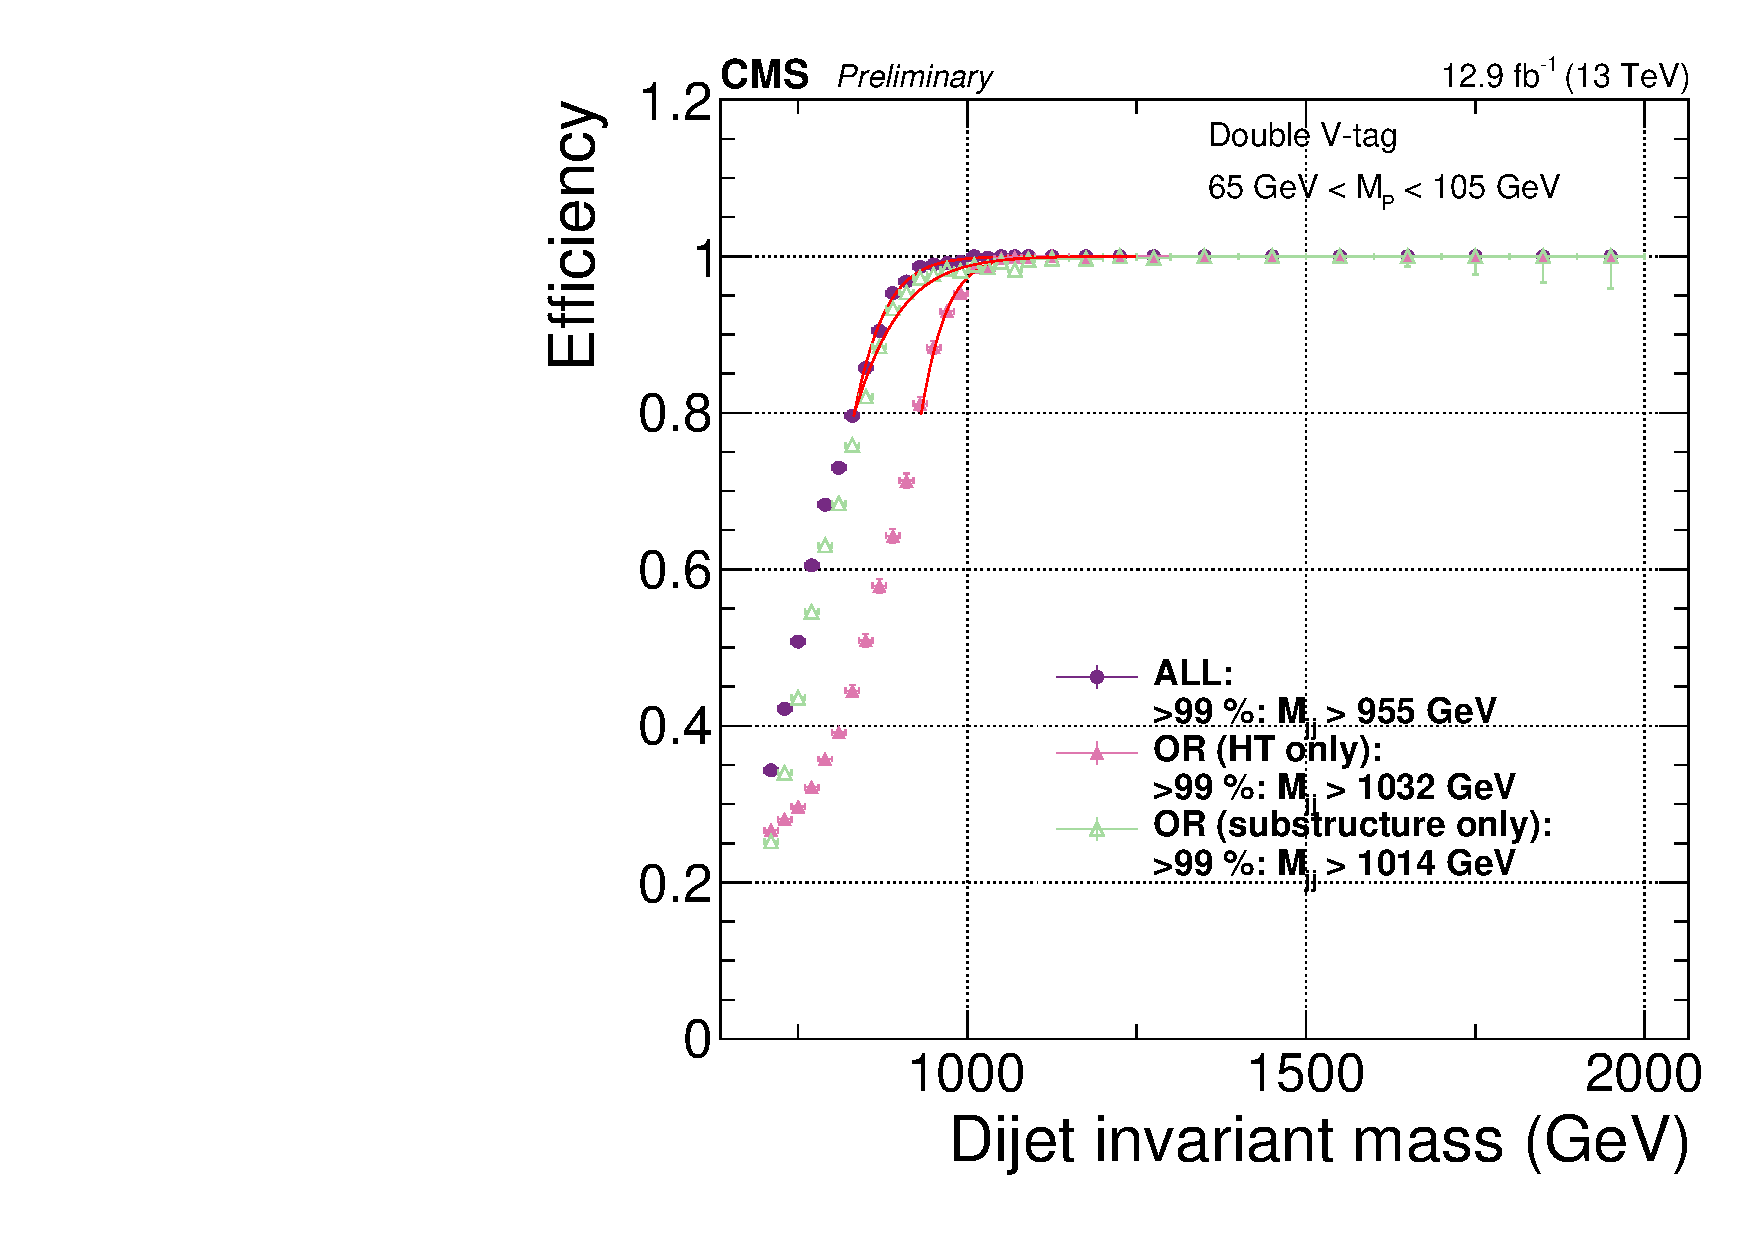
\includegraphics[width=0.49\textwidth]{figures/analysis/search2/AN-16-235/plots/triggereffMjj-ALL_DoubleTag.pdf}\\
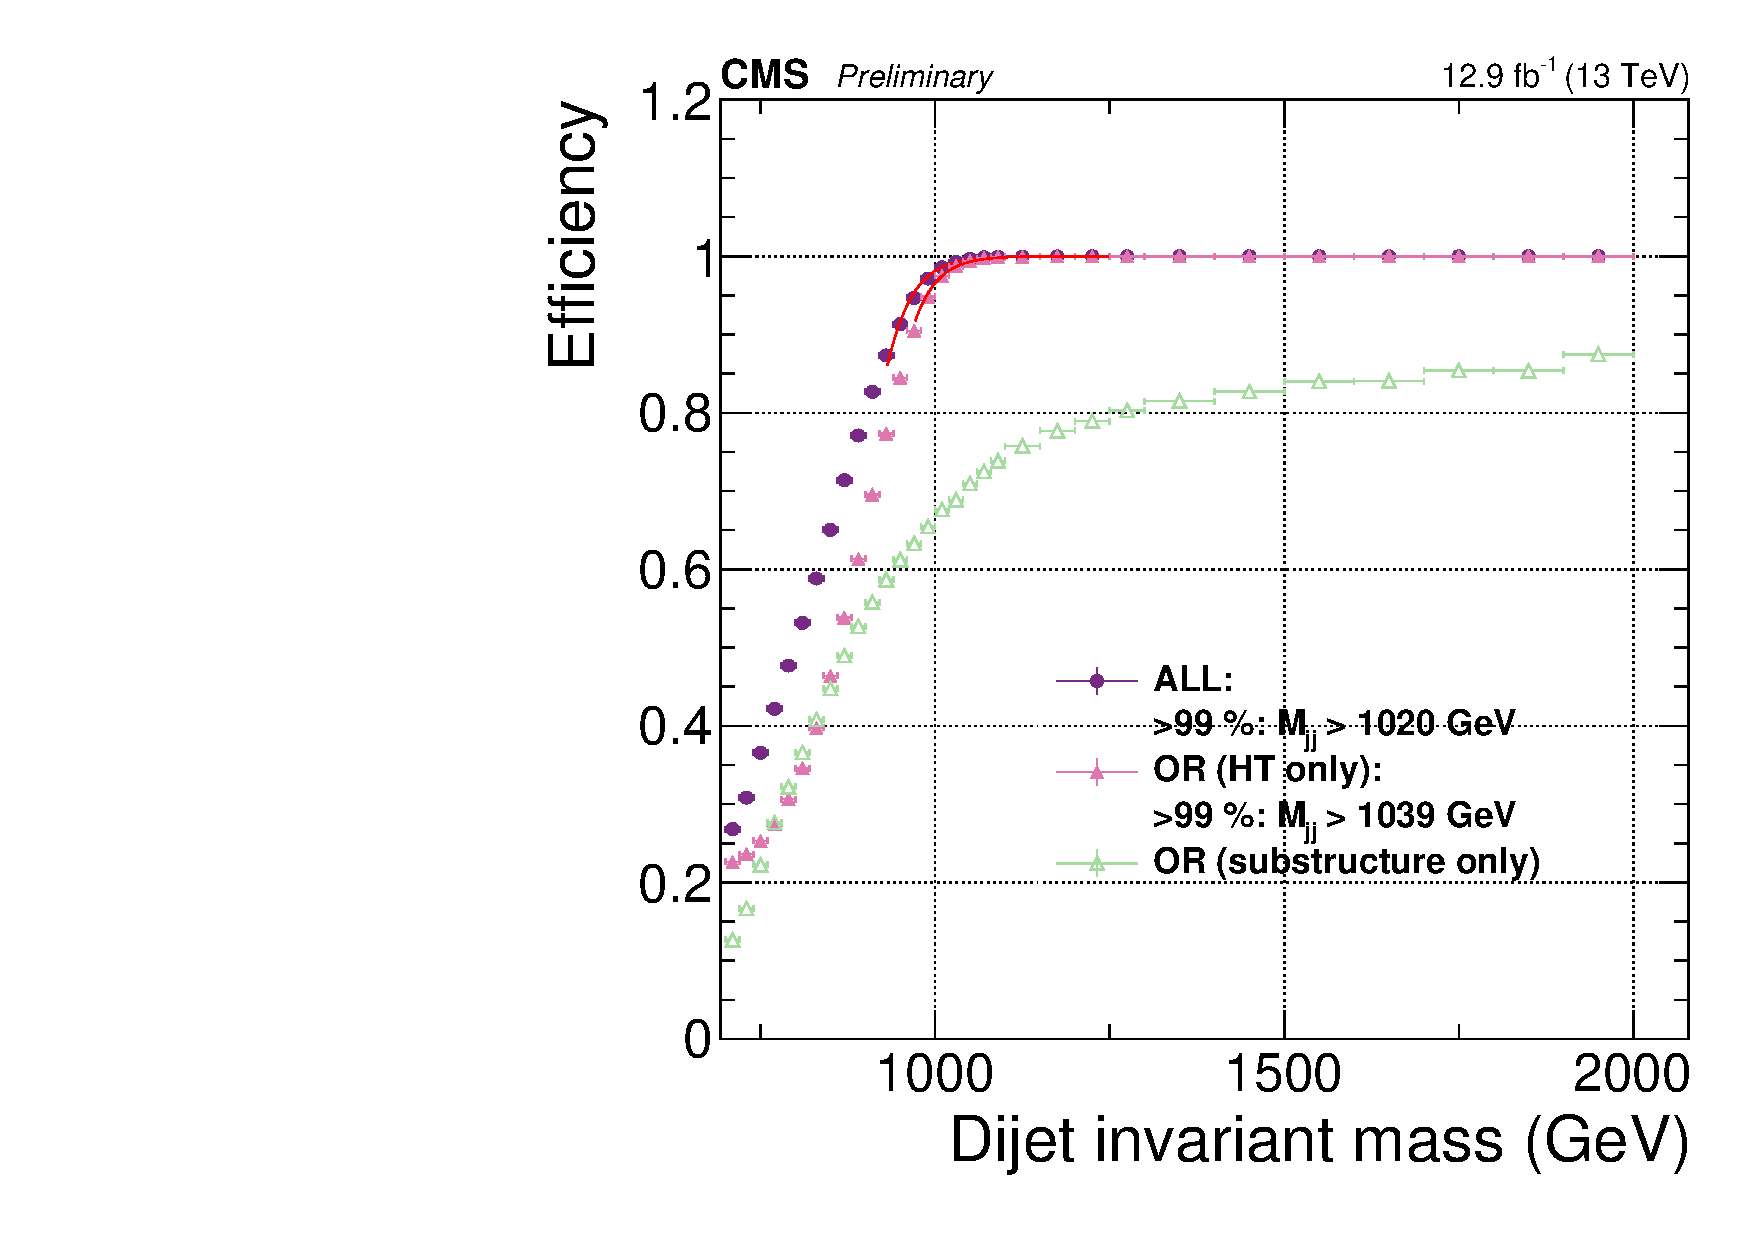
\includegraphics[width=0.49\textwidth]{figures/analysis/search2/AN-16-235/plots/triggereffMjj-ALL_noTag.pdf}
\caption{Comparison of trigger efficiencies for jets passing one of the HT-triggers only (pink), for jets passing one of the grooming-triggers only (green) and for jets passing one of the HT-triggers or one of the grooming triggers (purple). Here as a function of dijet invariant mass for all jet pairs passing loose selections and where one jet has a softdrop mass larger than 65 GeV (top left), both jets have a softdrop mass larger than 65 GeV (top right) and where no mass cut is applied (bottom). }
\label{fig:searchII:trigger-fits}
\end{figure}
Including grooming triggers lowers the 99\% trigger efficiency threshold by around 50(80) \GeV in the single (double) tag category once substructure is requested on the analysis level. Using the or of all triggers, we are safely on the trigger plateau for dijet invariant masses above 955(986) \GeV in the double (single) tag category, setting the analysis threshold at a dijet invariant mass of 955 \GeV for the double tag analysis and 990 \GeV for the single tag analysis. For controlplots, where no groomed mass window is applied, a trigger threshold of 1020 GeV is used.
\par Trigger efficiencies as a function of the offline softdrop-jet mass for the \\ 
\texttt{HLT\_AK8PFJet360\_TrimMass30} trigger are shown in Figure~\ref{fig:searchII:grooming-mj-trigger}. Here the jet transverse momentum of one of the jets is required to be at least 600 GeV and no other mass cut is applied. This trigger requires one jet to have a trimmed mass above 30 GeV at HLT level and reaches the trigger plateau for groomed-jet masses around 50 GeV. As reference trigger, the prescaled trigger \texttt{HLT\_PFJet320} is used. 
\begin{figure}[htb]
\centering
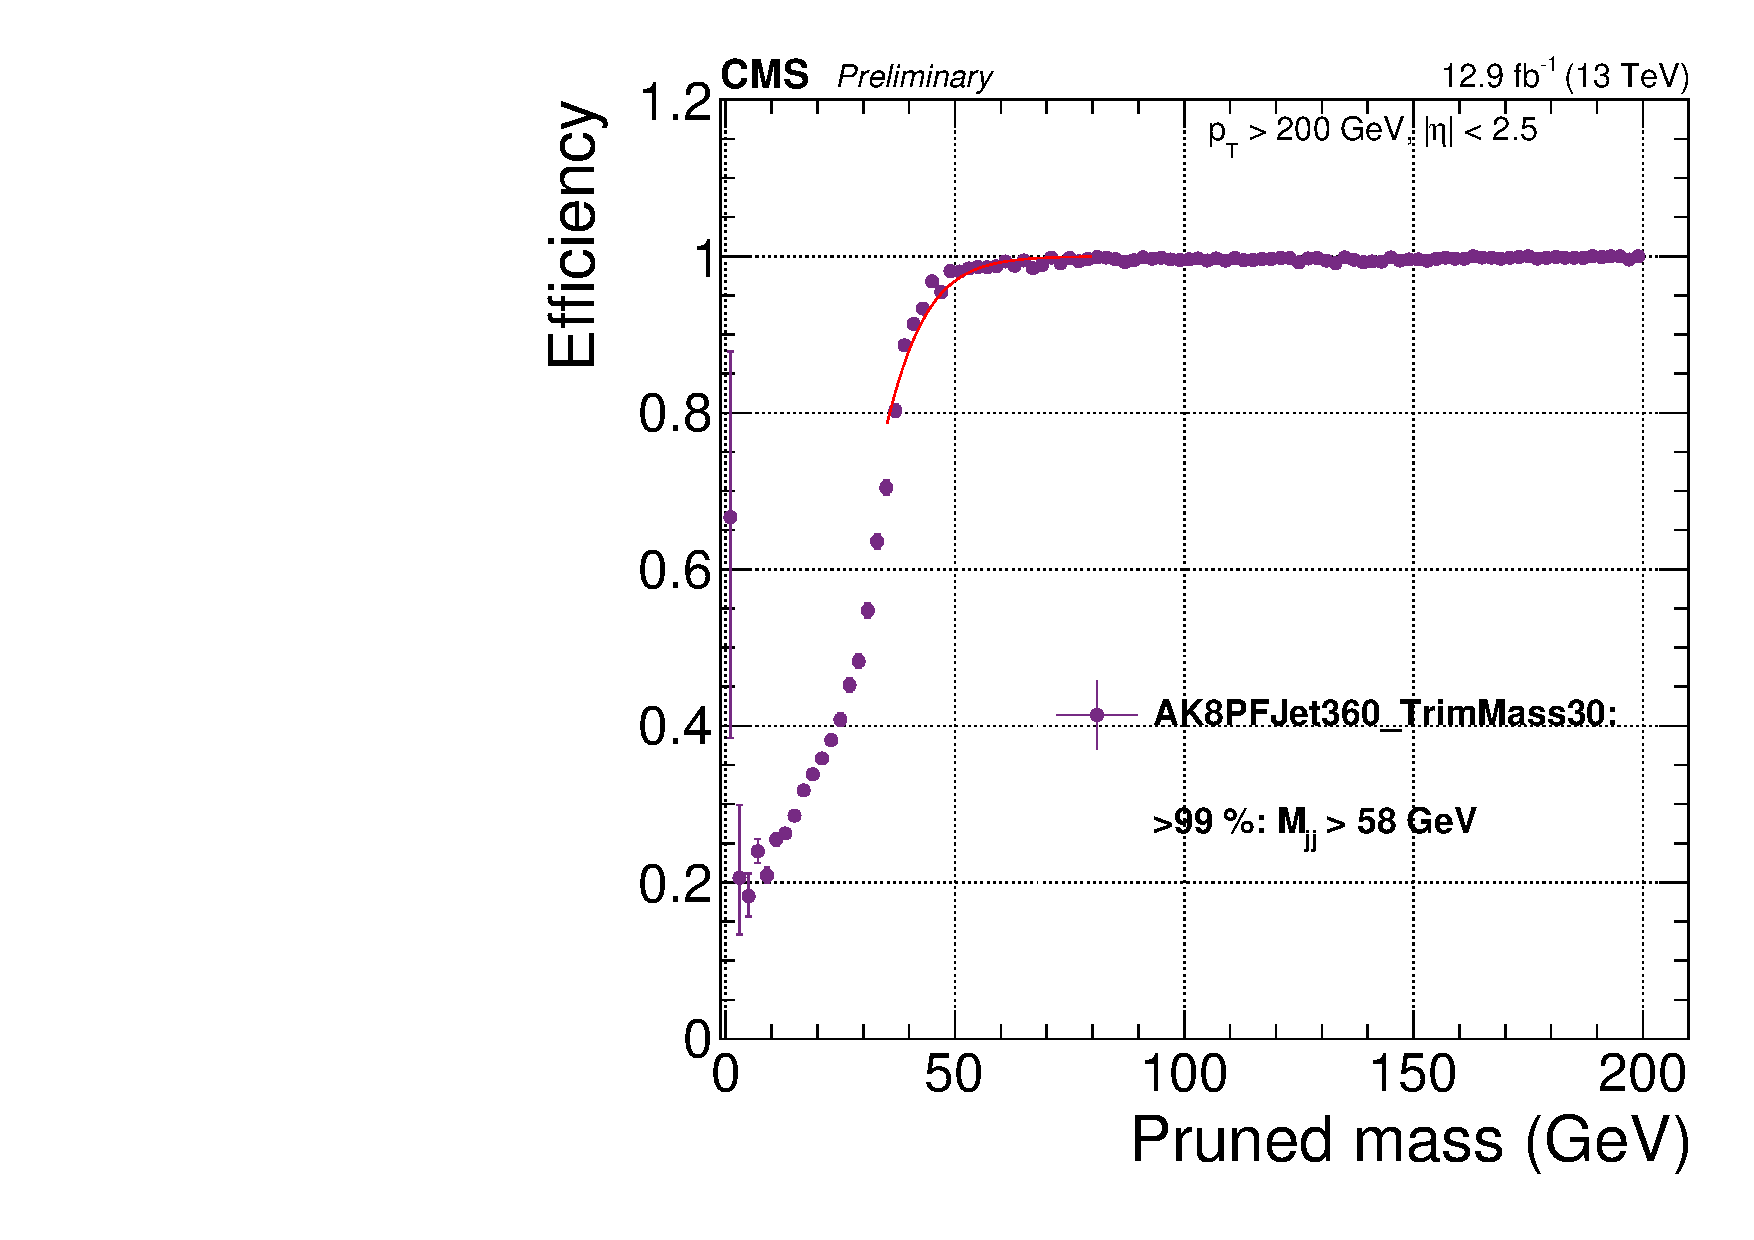
\includegraphics[width=0.49\textwidth]{figures/analysis/search2/AN-16-235/plots/triggereff-prunedmass_fit.pdf}
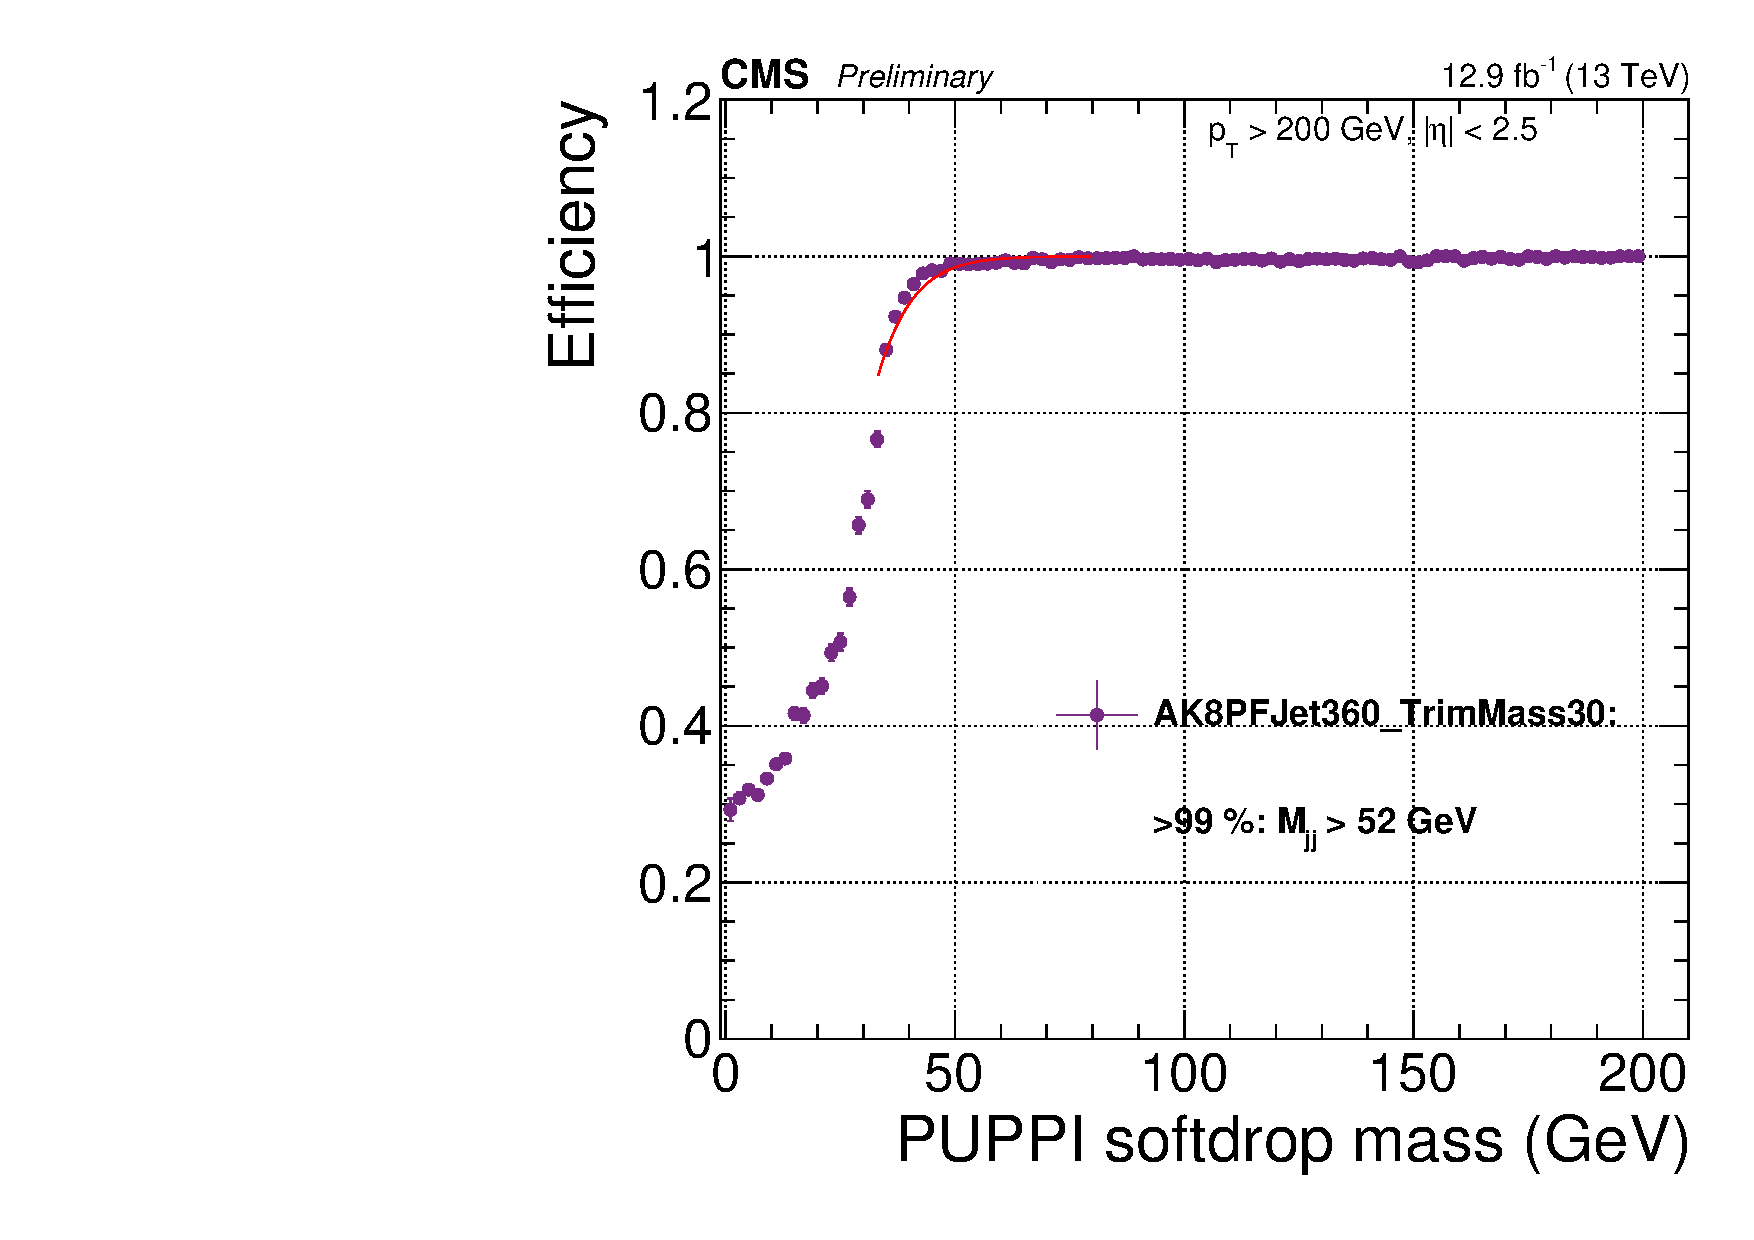
\includegraphics[width=0.49\textwidth]{figures/analysis/search2/AN-16-235/plots/triggereff-sdmass_fit.pdf}
\caption{Efficiency for the \texttt{HLT\_AK8PFJet360\_TrimMass30} trigger as a function of pruned-jet (left) and softdrop-jet (right) mass for jets with $\PT > \unit{600}{\GeV}$.}
\label{fig:searchII:grooming-mj-trigger}
\end{figure}

\subsubsection{Preselection}
\label{sec:searchII:presel}
The same preselections as in Search I, described in \label{sec:search1:preselection}, have been applied: We require two AK R=0.8 jets with CHS applied pre-clustering, required to pass the tight jet ID requirement, $\PT>200 \GeV$ and $|\eta|<2.5$. The same QCD t-channel suppressing cut of $|\Delta \eta|<1.3$ is required together with the following trigger thresholds on the dijet invariant mass: $\mjj > \unit{955} {\GeV}$ for the double V-tag and $\unit{990} {\GeV}$ for the single V-tag analysis. The jet \PT (top left), $\eta$ (top right), $\Delta \eta_{jj}$ and dijet invariant mass (bottom left) for the two leading jets in the event after loose preselections are applied is shown in Figure~\ref{fig:searchII:kinematics-all}.
\begin{figure}[h!]
\centering
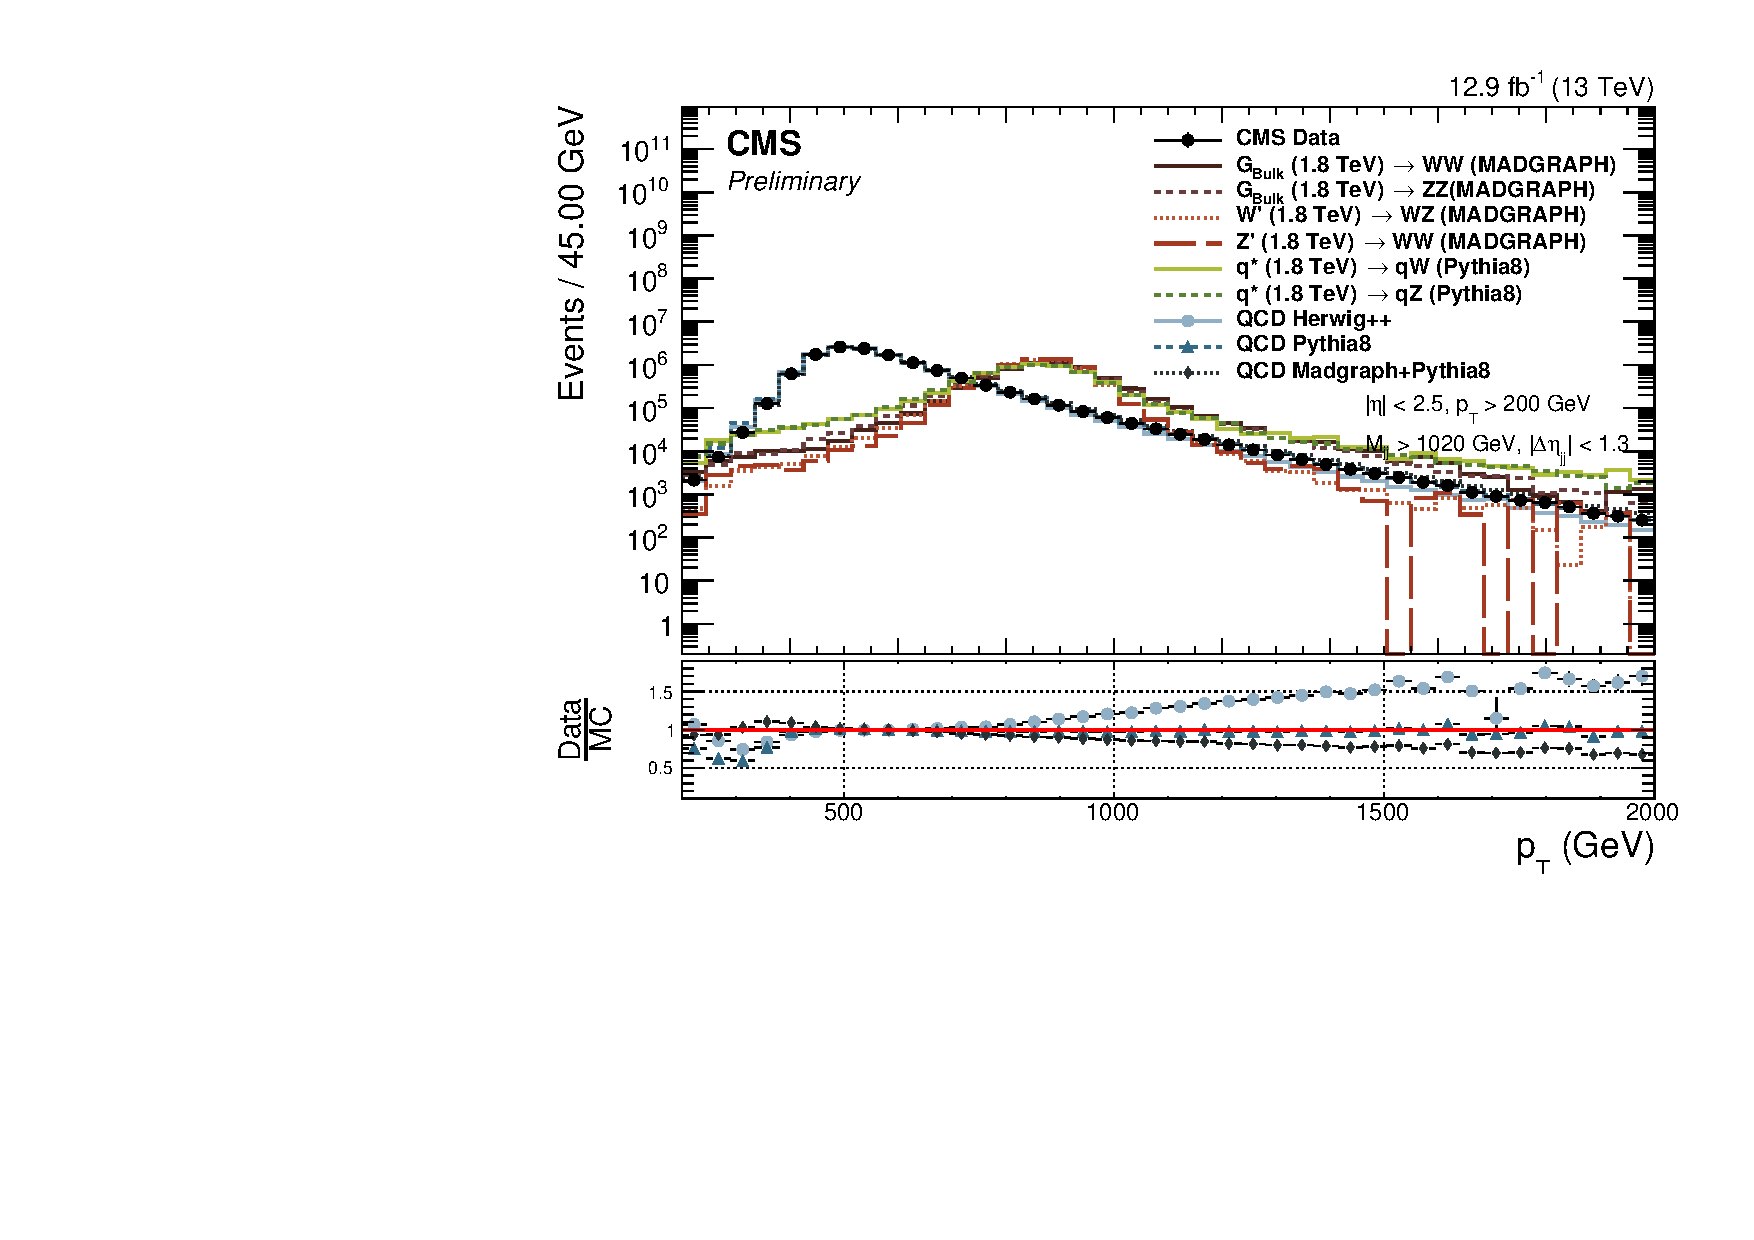
\includegraphics[width=0.49\textwidth]{figures/analysis/search2/AN-16-235/plots/qcdcp_Pt.pdf}
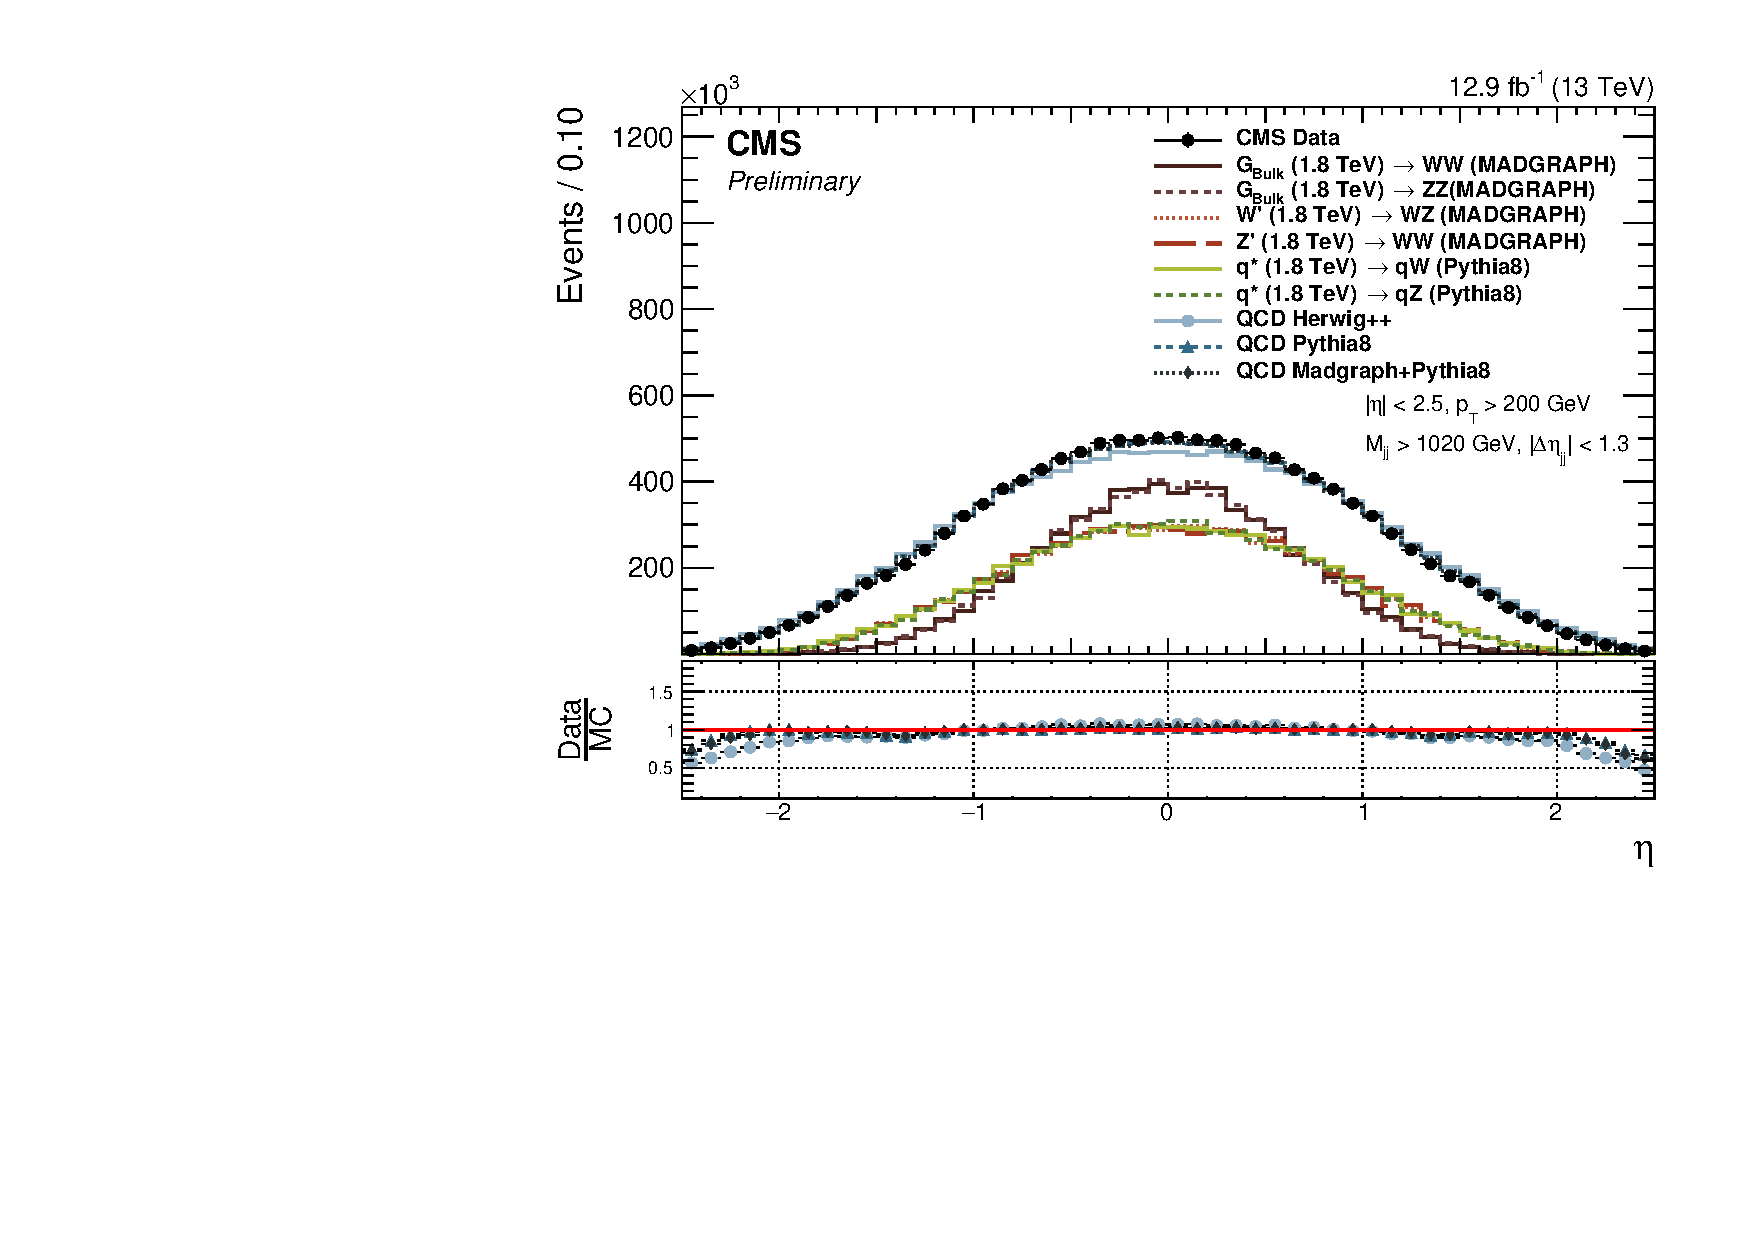
\includegraphics[width=0.49\textwidth]{figures/analysis/search2/AN-16-235/plots/qcdcp_Eta.pdf}\\
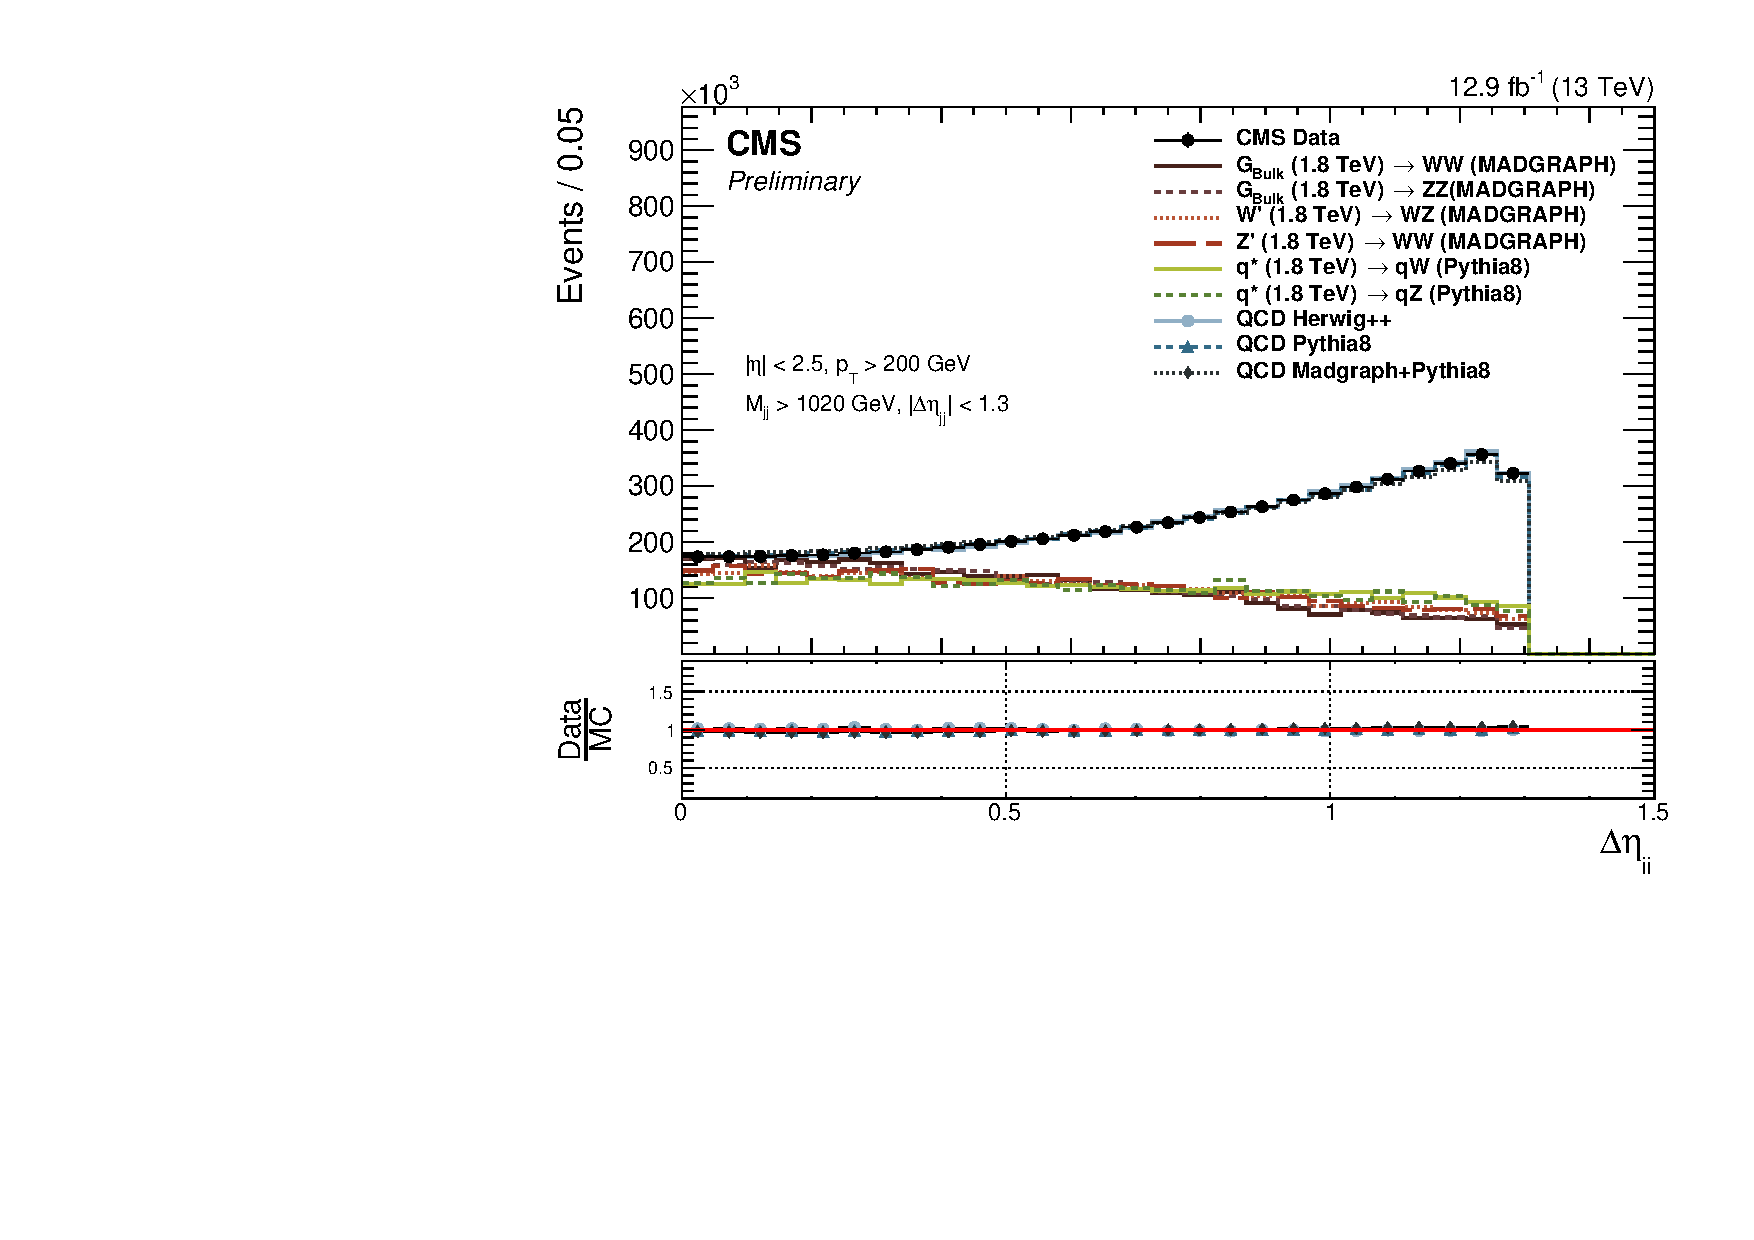
\includegraphics[width=0.49\textwidth]{figures/analysis/search2/AN-16-235/plots/qcdcp_DeltaEta.pdf}
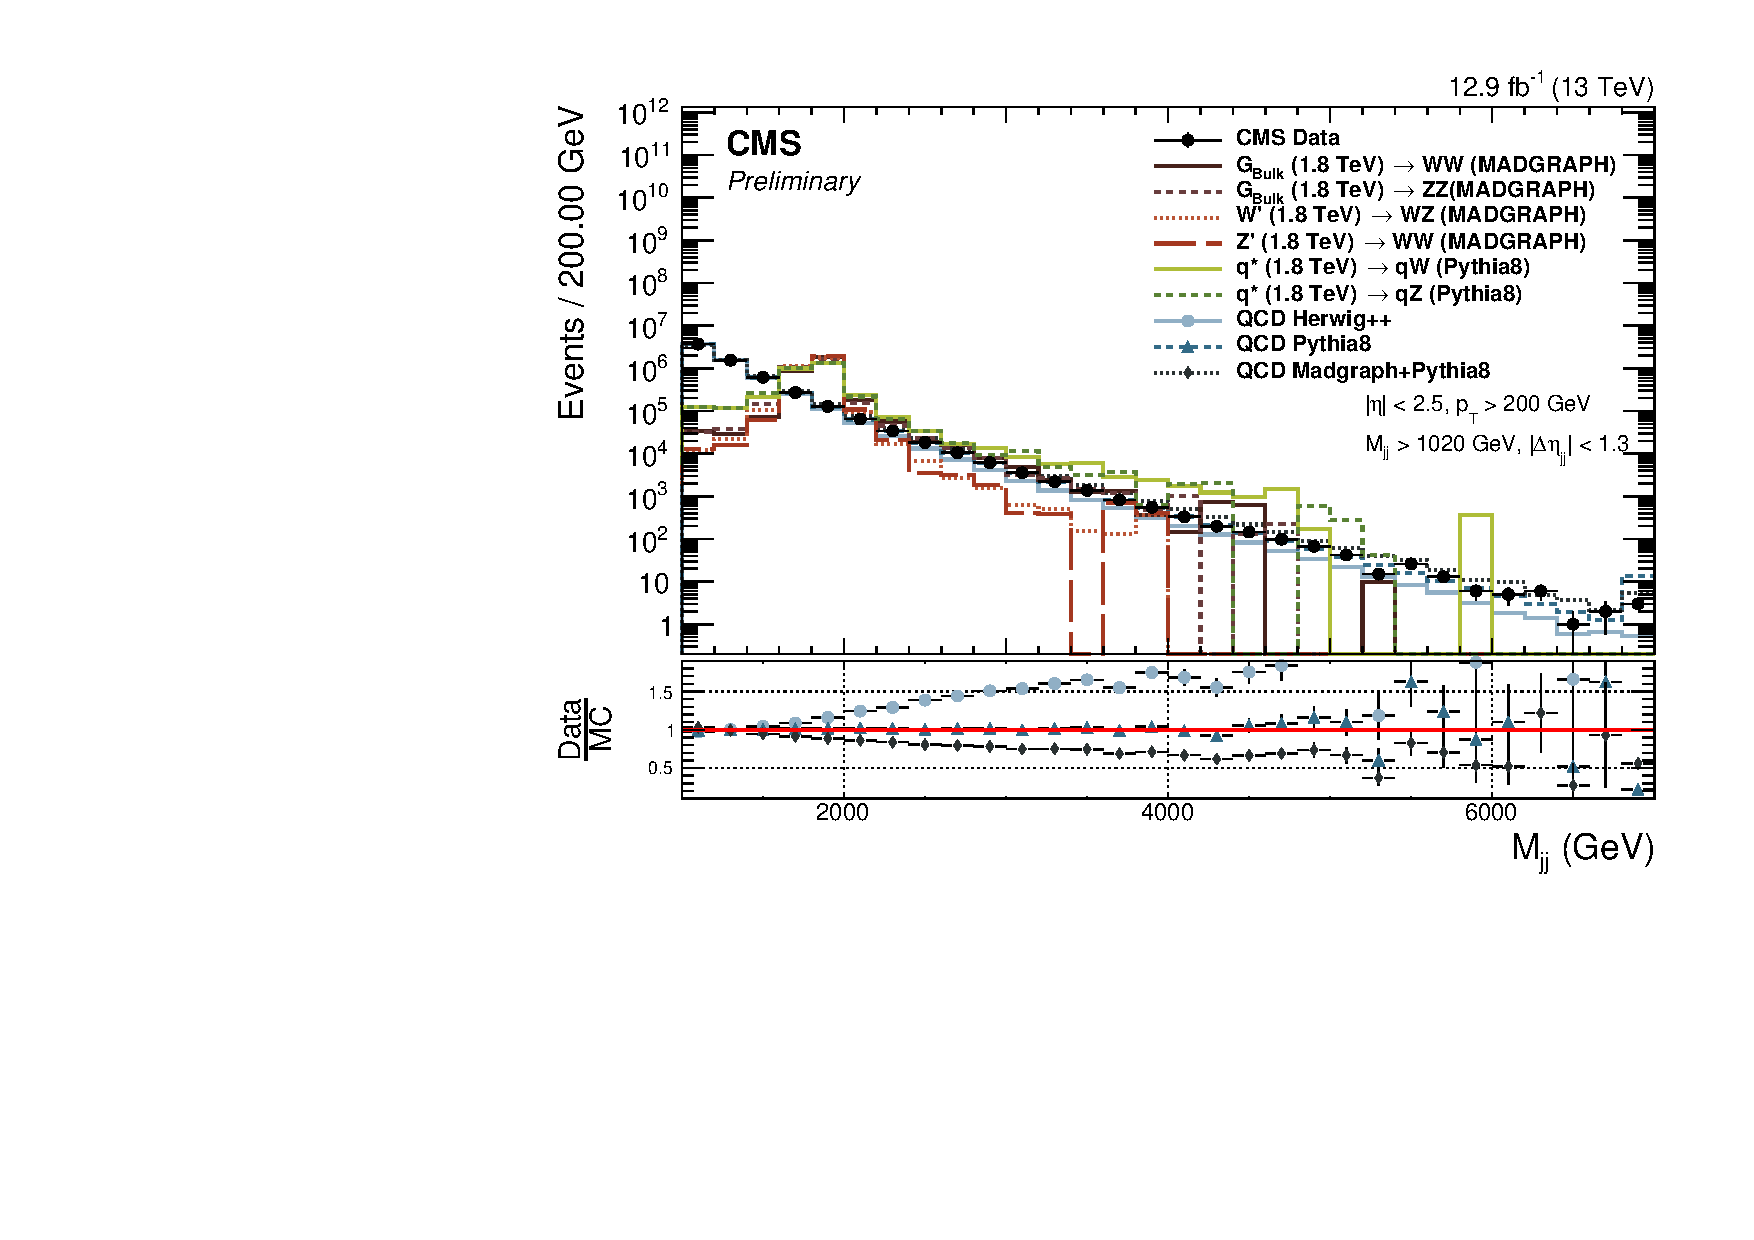
\includegraphics[width=0.49\textwidth]{figures/analysis/search2/AN-16-235/plots/qcdcp_Mjj.pdf}
\caption{Jet \PT{} (top left), $\eta$ (top right), $\Delta \eta_{jj}$ and dijet invariant mass (bottom left) for the two leading jets in the event after loose preselections are applied. The signal is scaled by an arbitrary number.}
\label{fig:searchII:kinematics-all}
\end{figure}
A large difference in slope in the jet \PT and dijet invariant mass spectrum depending on the QCD matrix element or shower generator is observed. Pure \PYTHIA QCD MC describes the data best, while \HERWIG{++} and \amcatnlo{}+\PYTHIA tend to under- or over-estimate the number of high $\PT/\mjj$ jets, respectively. Pure \PYTHIA QCD MC is therefore used for all background checks in this analysis.


\subsection{Developing a new W-tagger}
\label{sec:searchII:puppisoftdrop}
As mentioned in the introduction to this chapter, early studies had shown that the PUPPI pileup subtraction algorithm yielded superior resolution on large-cone jet observables like the jet mass. We therefore wanted to check whether the softdrop jet mass, and its observed sensitivity to the Underlying Event and pileup, would be improved if a better pileup subtraction algorithm was applied pre-clustering.\par
Two interesting observations were made. Softdrop used together with PUPPI pileup subtraction displayed a much smaller \PT-dependent shift than CHS+Softdrop, as hoped. Figure~\ref{fig:searchII:sdmass} shows the PUPPI softdrop mass for W-jets from a 1 \TeV ($\PT\sim 500 \GeV$) and 4 \TeV ($\PT\sim 2 \TeV$) resonance, exhibiting the desired reduced \PT dependence in jet mass scale. 
\begin{figure}[htb]
\centering
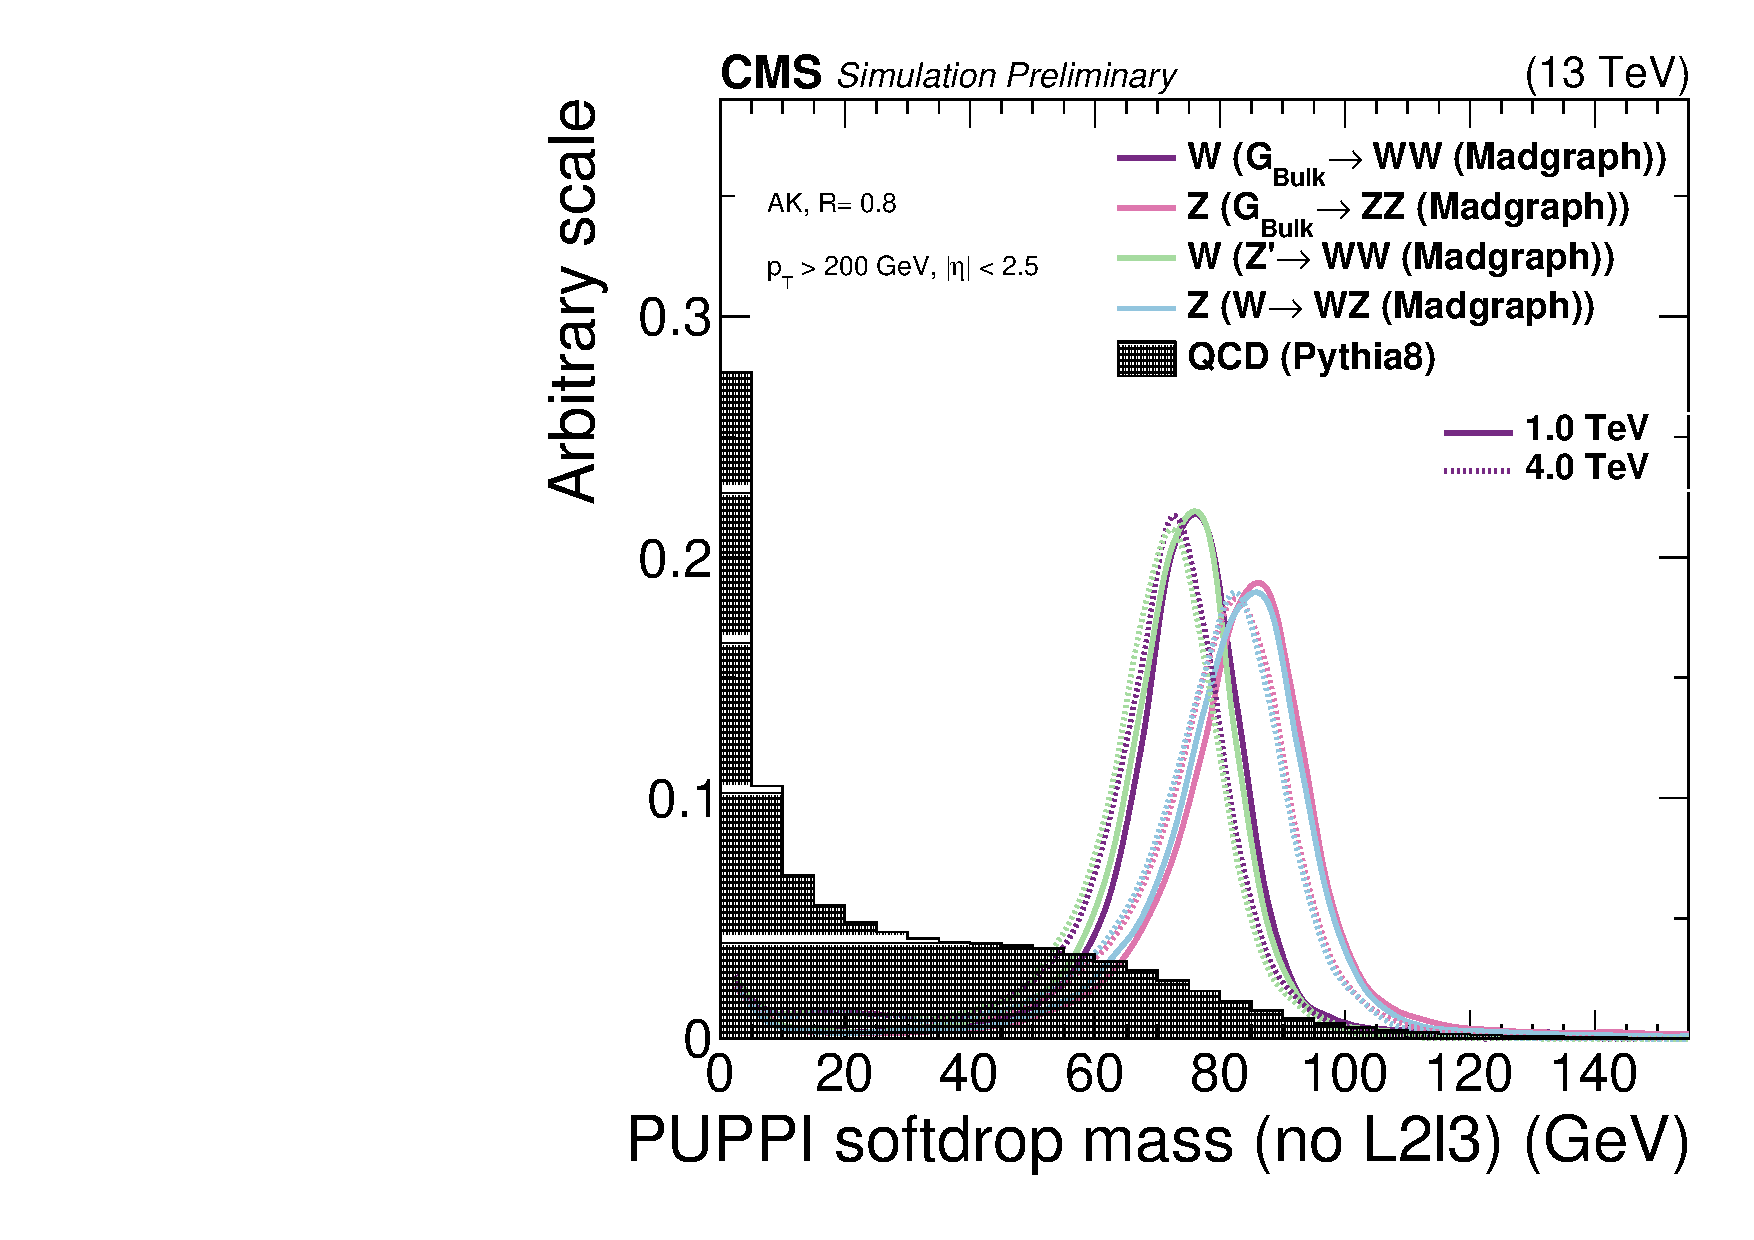
\includegraphics[width=0.49\textwidth]{figures/analysis/search2/AN-16-235/plots/gen_SoftdropMassUnCorr.pdf}
\caption{The  PUPPI softdrop jet mass distribution with no jet energy corrections applied}
\label{fig:searchII:sdmass}
\end{figure}
However, when applying centrally provided L2 and L3 jet energy corrections (see Section~\ref{sec:objreco:jec}) to the jet groomed mass, as is recommended, a strong \PT dependence is re-introduced. This effect is not present for the pruned jet mass. Figure~\ref{fig:searchII:wtagmass} show the softdrop (top left) and pruned (top right) jet mass distribution with recommended L2L3 corrections applied. Here, the PUPPI+softdrop jet mass shift is significantly increased with respect to what was observed for the uncorrected mass, while CHS+pruned jet mass is stable. This points to the PUPPI jet energy corrections not being optimal for scalar jet mass variables, while they may be good for correcting jet 4-vectors. The jet energy corrections derived for CHS and PUPPI jets as a function of jet \PT is shown in the bottom plot in Figure~\ref{fig:searchII:wtagmass} . A significant slope in JEC as a function of \PT is measured for PUPPI, while not present for CHS.
\begin{figure}[htb]
\centering
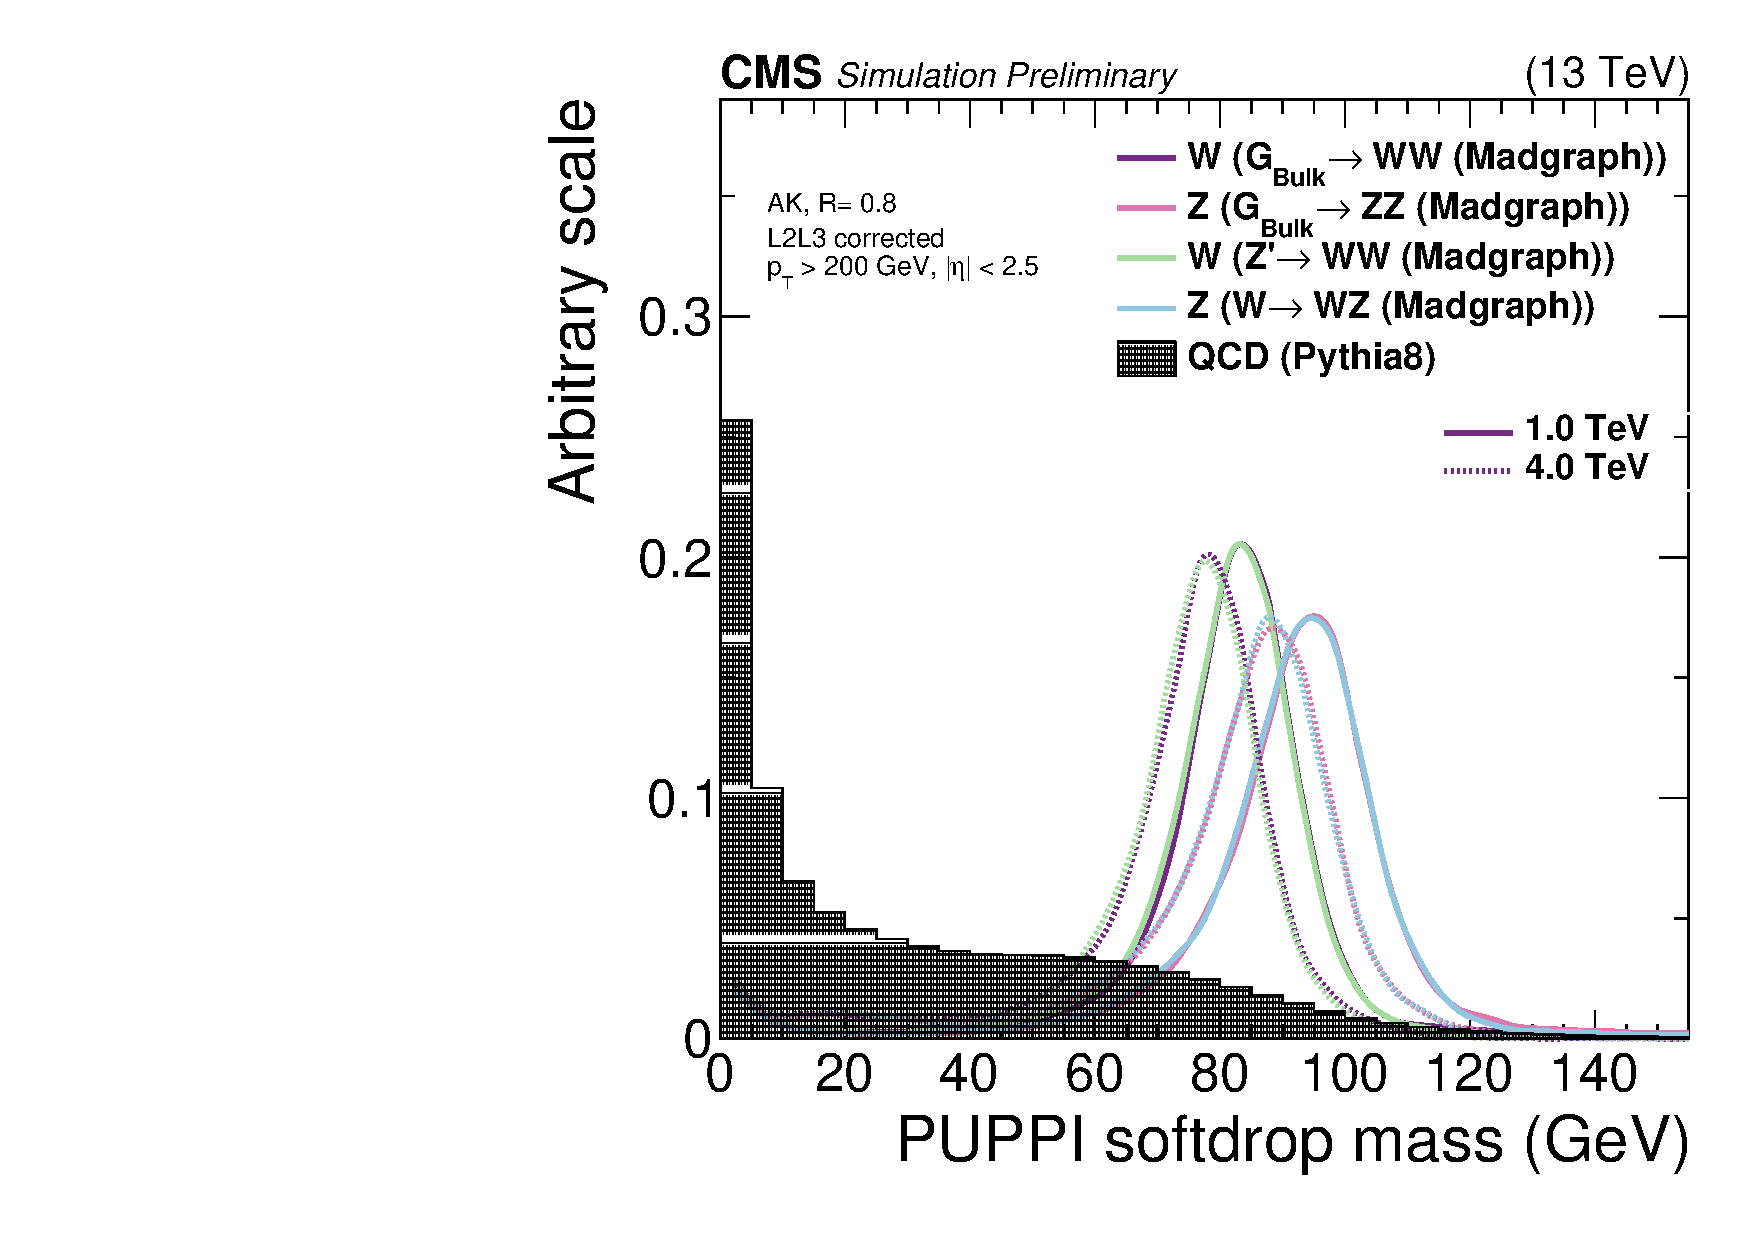
\includegraphics[width=0.49\textwidth]{figures/analysis/search2/AN-16-235/plots/gen_SoftdropMass.pdf}
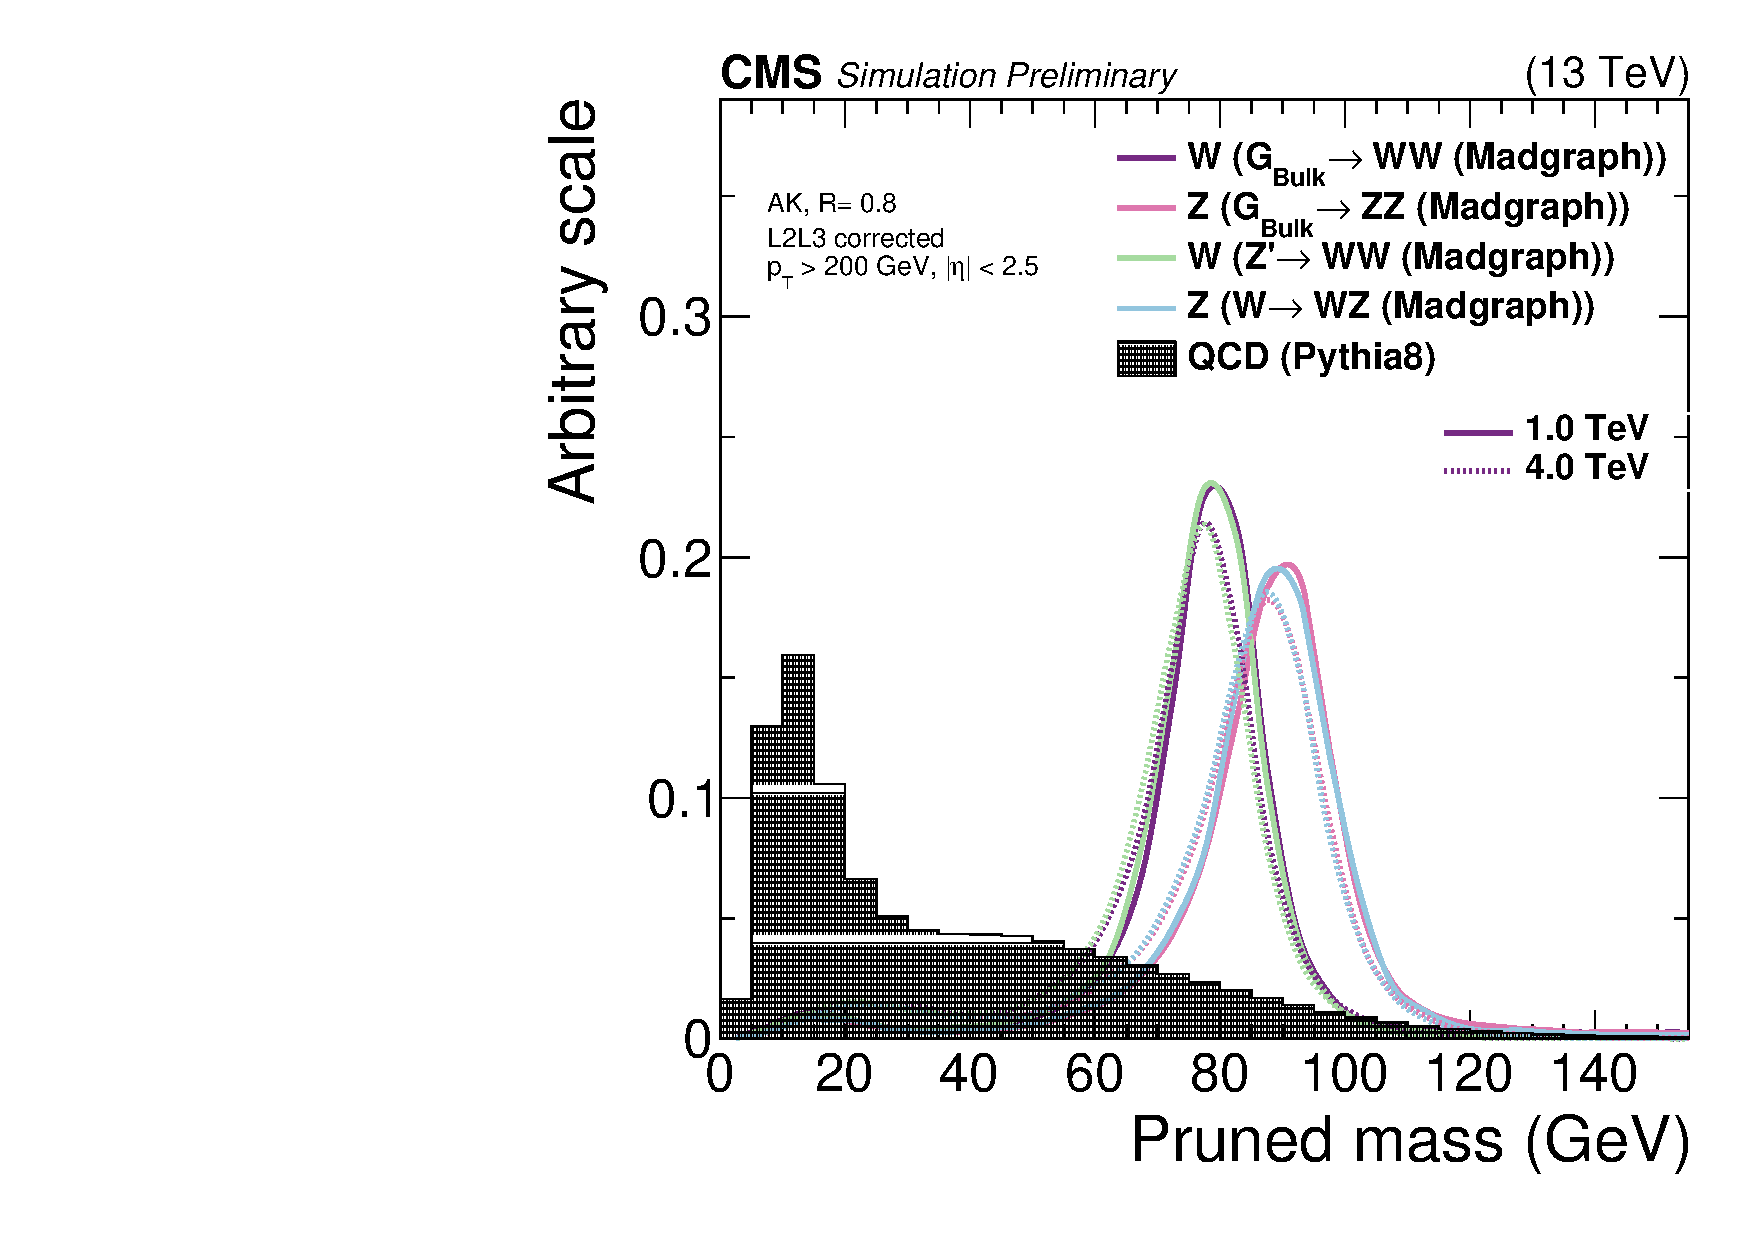
\includegraphics[width=0.49\textwidth]{figures/analysis/search2/AN-16-235/plots/gen_PrunedMass.pdf}\\
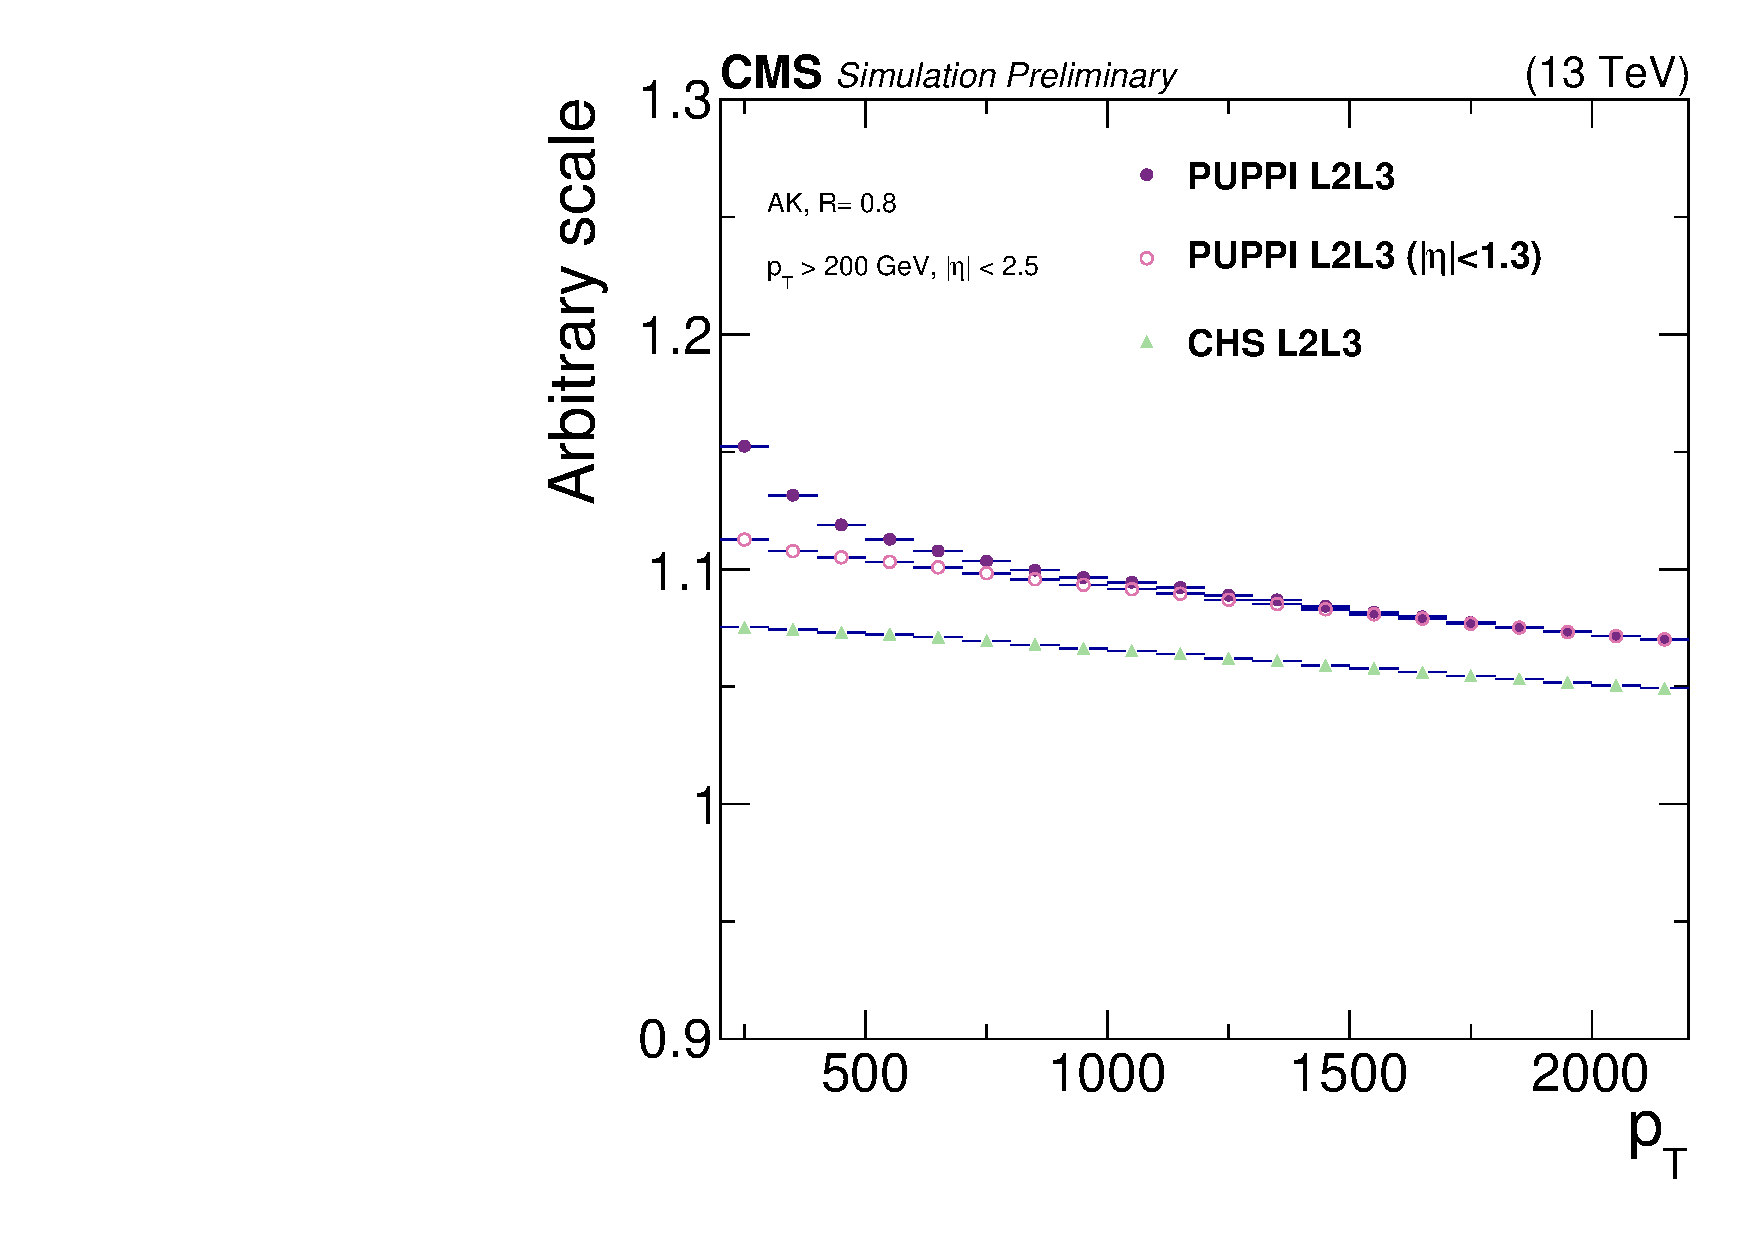
\includegraphics[width=0.49\textwidth]{figures/analysis/search2/AN-16-235/plots/JECvsPT.pdf}
\caption{Top: PUPPI softdrop mass distribution (top left) and pruned jet mass distribution (top right) with L2 and L3 corrections applied. Bottom: The projection of CHS and PUPPI jet energy corrections versus jet \PT.}
\label{fig:searchII:wtagmass}
\end{figure}

\subsubsection{Dedicated PUPPI softdrop mass corrections}
\label{sec:searchII:masscorr}
In order to minimize \PT dependence in the PUPPI softdrop jet mass, all jet energy corrections to the softdrop jet mass are removed. However, this still leaves a residual \PT dependence and, in addition, the uncorrected mass does not peak at the correct W-mass of 80.4~\GeV. Figure~\ref{fig:searchII:UncorrSD} shows the mean of a Gaussian fit to the uncorrected PUPPI softdrop mass as a function of jet $\pt$ in two different $\eta$ bins (smaller or greater than $|\eta|=1.3$) for W-jets coming from a Bulk Graviton signal sample. A mass shift both as a function of $\eta$ and \PT is observed, together with an average mean significantly lower than the W-mass.
\begin{figure}[htbp]
\centering
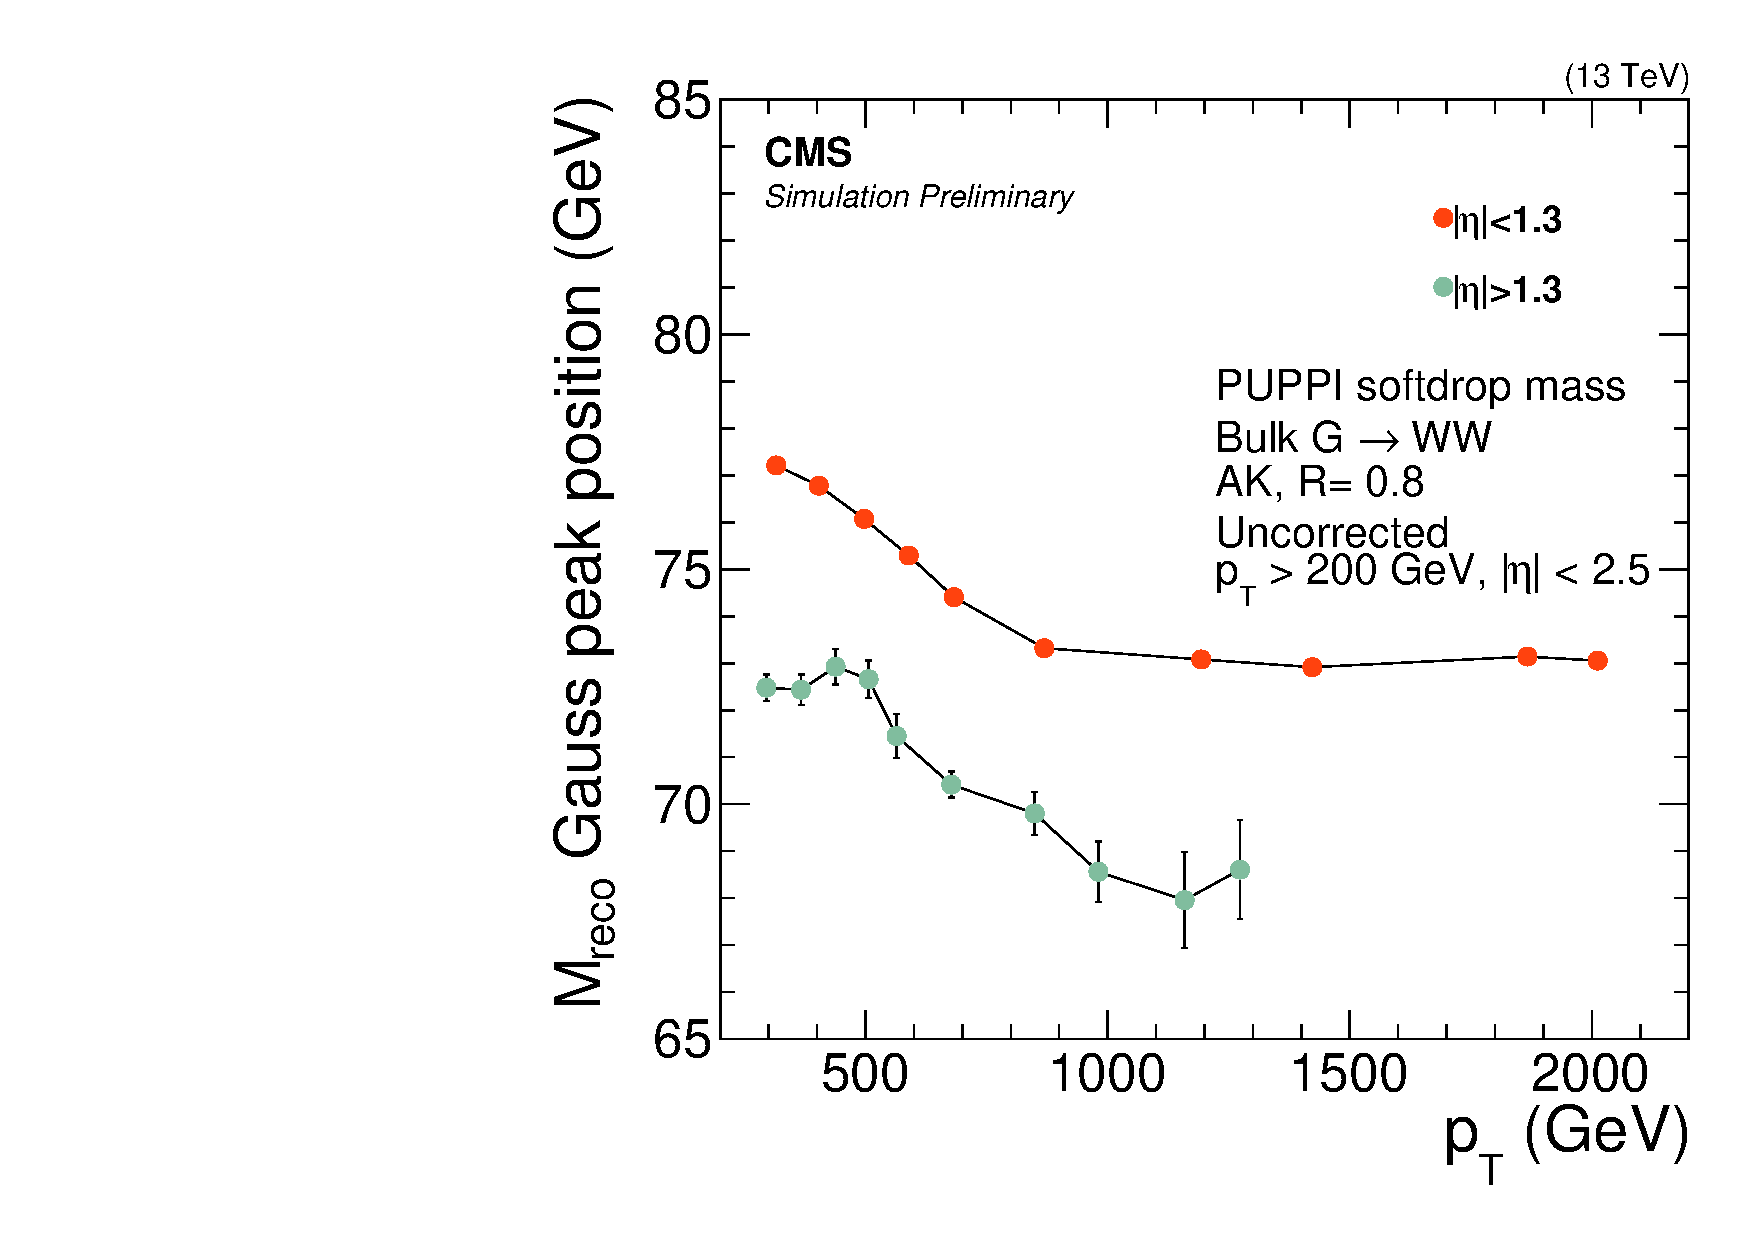
\includegraphics[width=0.49\textwidth]{figures/analysis/search2/AN-16-235/plots/RecoPuppiSoftdropMass_vspt.pdf}
\caption{The mean of a Gaussian fit to the W-jet PUPPI softdrop mass peak as a function of jet \PT in two different $\eta$ bins (smaller or greater than $|\eta|=1.3$). No corrections have been applied to the softdrop mass.}
\label{fig:searchII:UncorrSD}
\end{figure}
In order to use PUPPI+softdrop for W-tagging, we therefore derive dedicated jet mass corrections to compensate for two factors: A generator level \PT-dependence, as first observed in \label{sec:searchI:wtagging}, and a reconstruction level \PT- and $\eta$-dependence, most likely caused by UE effects and the growing effective sofdrop radius at low jet \PT. Figure~\ref{fig:searchII:sdmassshifts} shows the mean of the generated softdrop mass (left) and the normalized difference in reconstructed and generated softdrop mass (right) as a function of jet \PT. The shift in generated softdrop mass at lower \PT is of the order of 2-3$\%$ while the difference between reconstructed and generated softdrop mass is a 5-10$\%$ effect.
\begin{figure}[htbp]
\centering
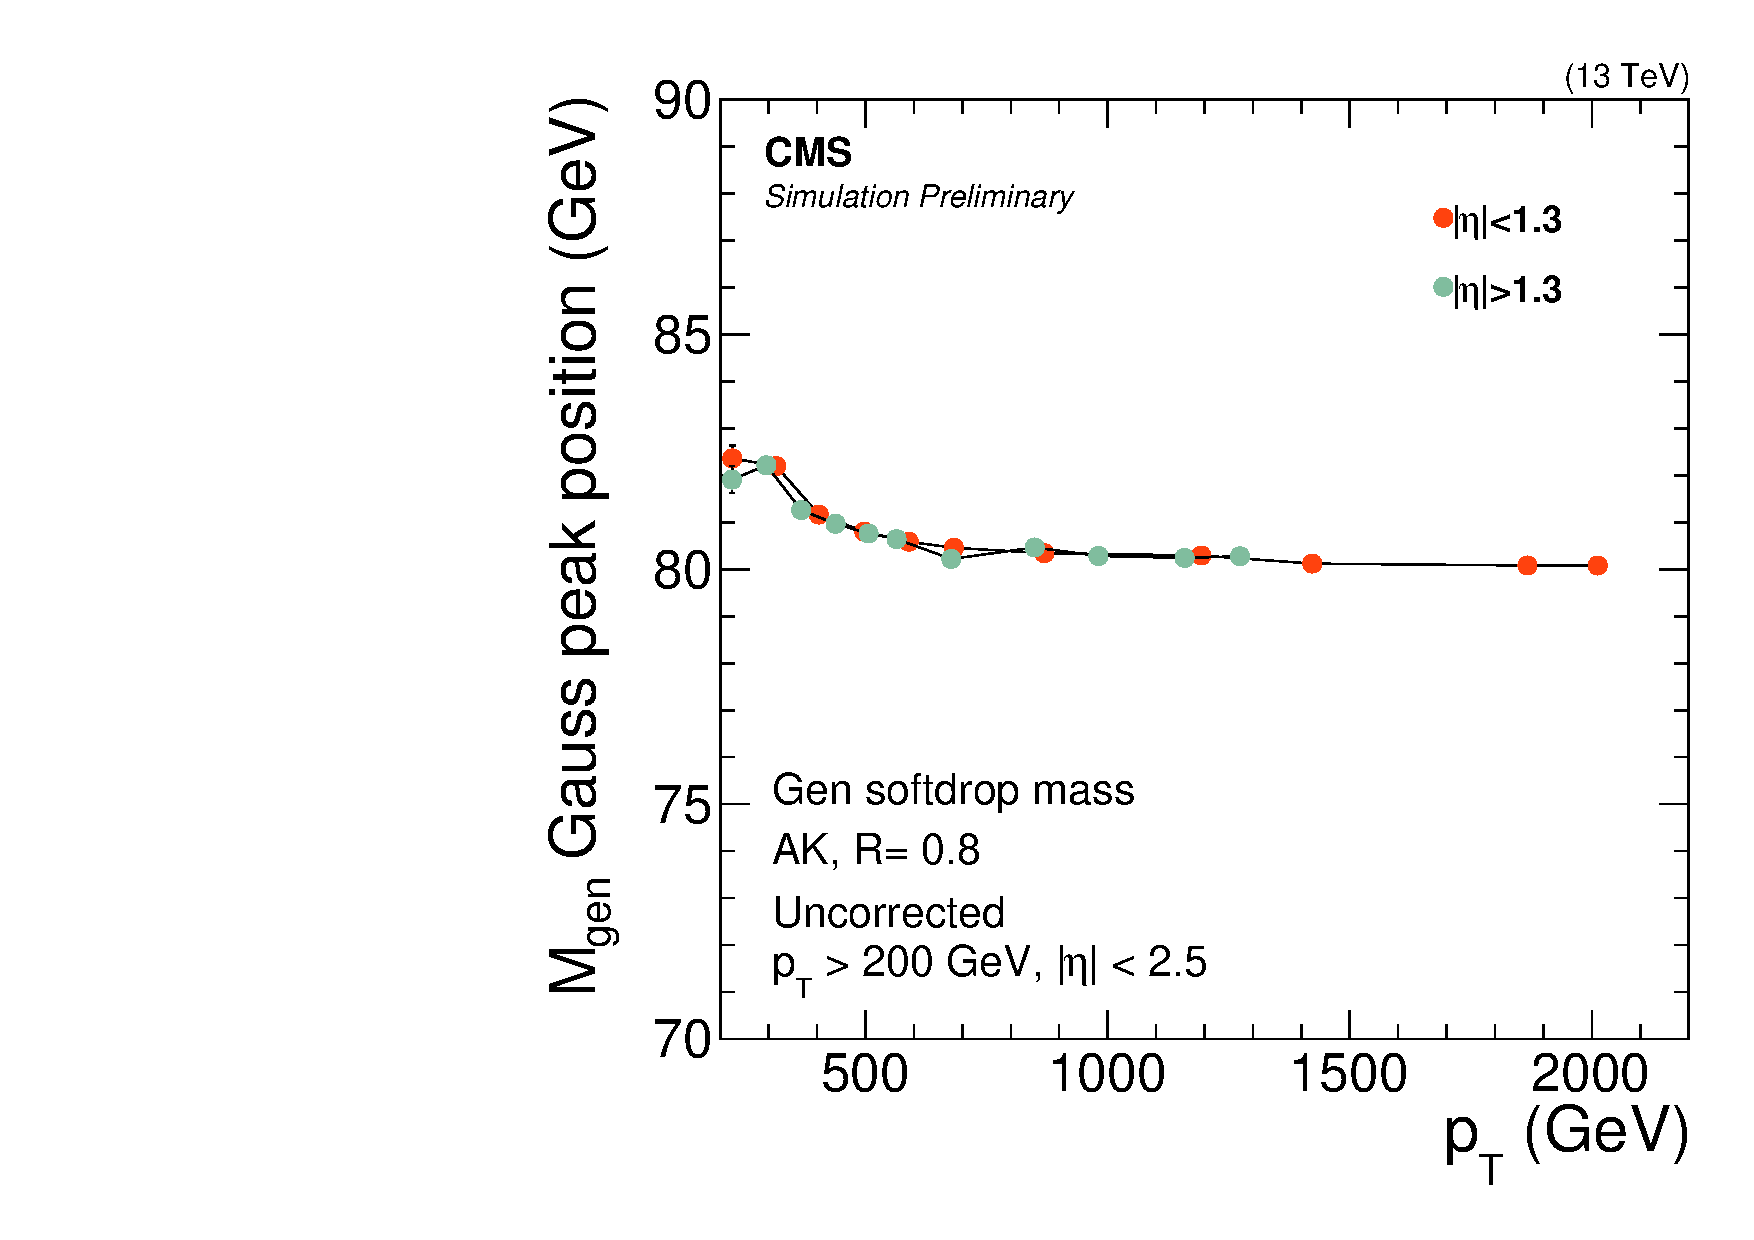
\includegraphics[width=0.49\textwidth]{figures/analysis/search2/AN-16-235/plots/GenSoftdropMass_vspt.pdf}
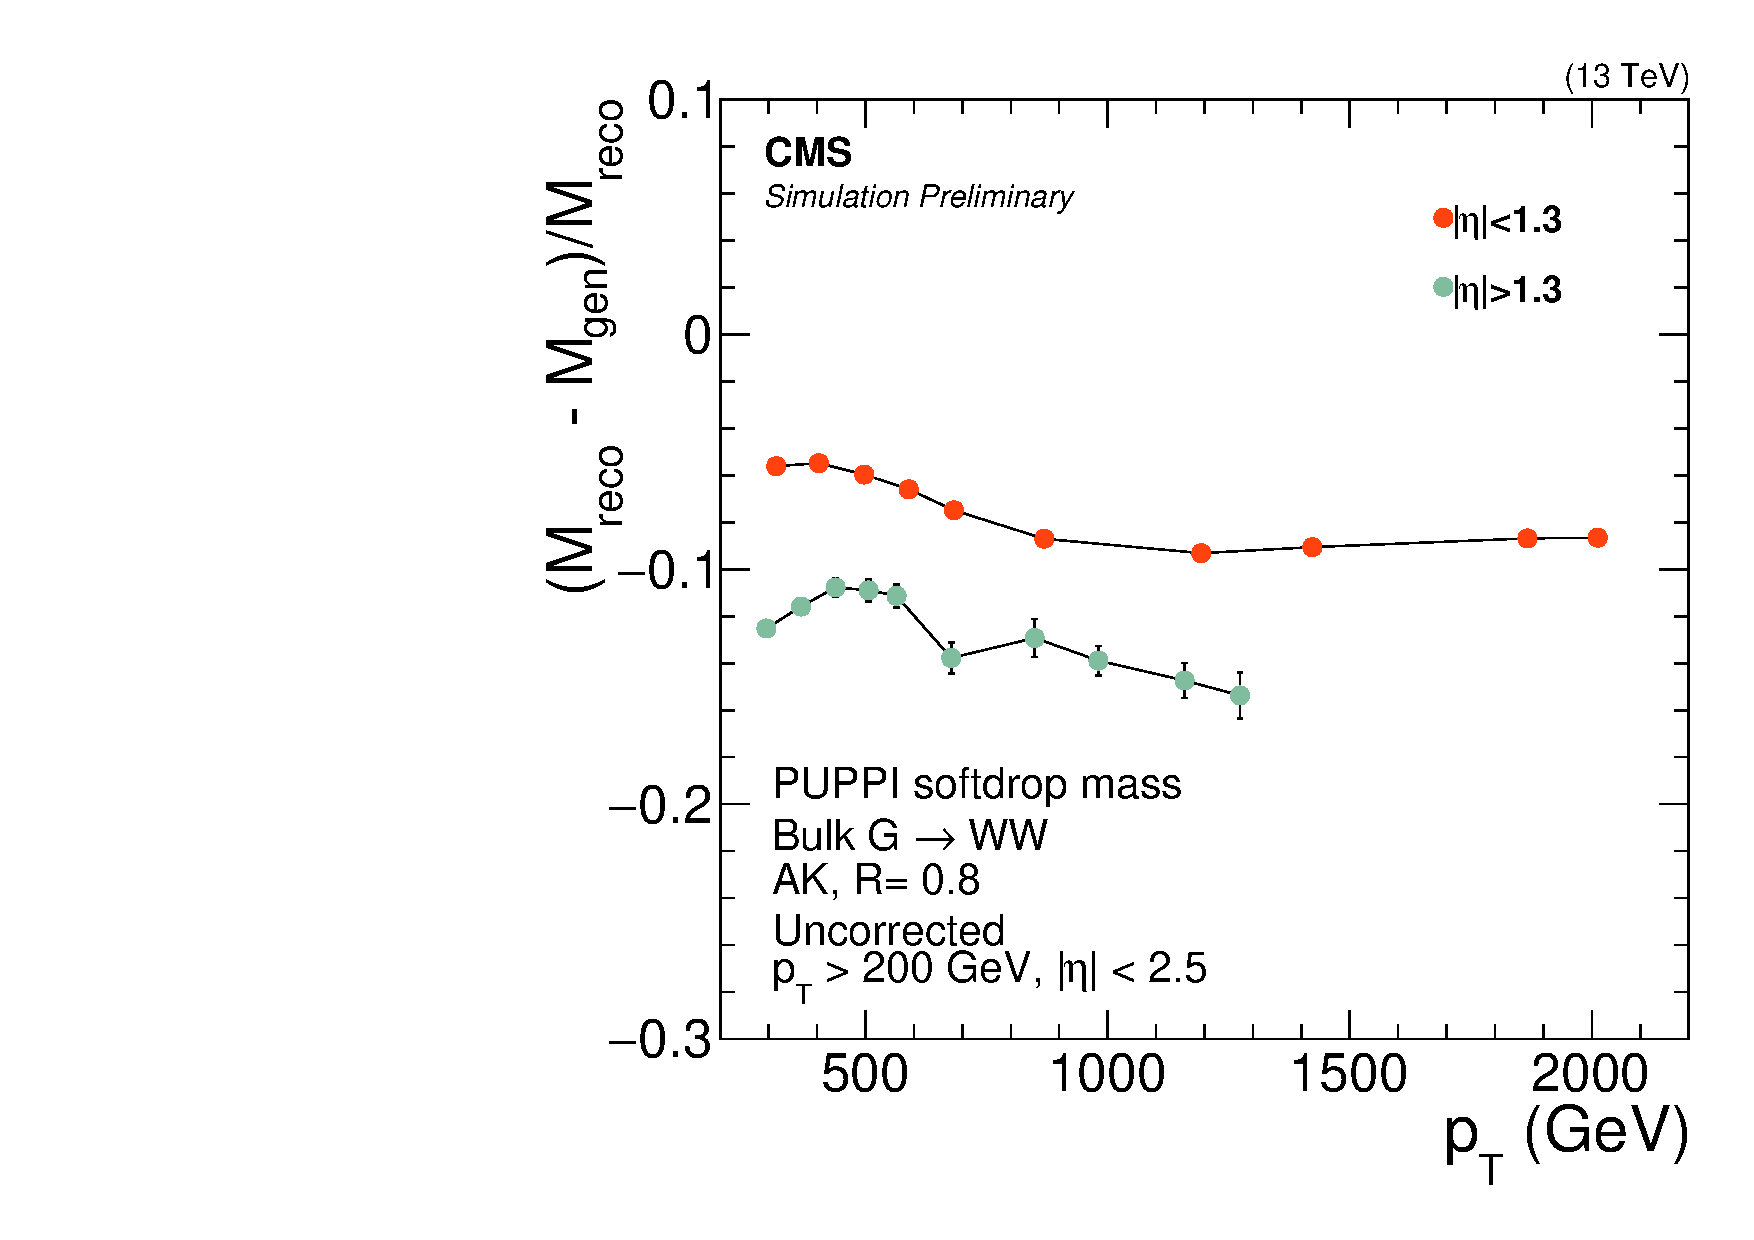
\includegraphics[width=0.49\textwidth]{figures/analysis/search2/AN-16-235/plots/MassShift_vspt.pdf}
\caption{The mean of the fitted generator level W-jet softdrop mass distribution as a function of jet $\pt$ (left) and the normalized difference in reconstructed and generated softdrop mass (right).}
\label{fig:searchII:sdmassshifts}
\end{figure}
The mass shift introduced at generator level is corrected by a fit to $\rm{M_{PDG}/M_{GEN}}$ as a function of jet \PT, where $\rm{M_{PDG}}=80.4~\GeV$ and $\rm{M_{GEN}}$ is the fitted mean of the generator level mass as shown in the left plot in Figure~\ref{fig:searchII:sdmassshifts}. To correct for the residual shift between generated and reconstructed softdrop mass, a fit to $\rm{(M_{RECO}-M_{GEN})/M_{RECO}}$, where $\rm{M_{RECO}}$ is the reconstructed mass shown in the right plot in Figure~\ref{fig:searchII:sdmassshifts} and $\rm{M_{GEN}}$ is as defined above, as a function of jet \PT in two $\eta$ bins (smaller or greater than $|\eta|=1.3$) is performed.
Polynomial fit functions of the following forms are used
\begin{align*} 
% w(\pt) &=  [0]+[1]*pow(x*[2],-[3] \\
w(\pt) &=  A  +B(x^{2})^{-C}          &\sim\textrm{``gen correction''}\\
w(\pt) &=  A  +Bx+Cx^2+Dx^3+Ex^4+Fx^5 &\sim\textrm{``reco correction''} 
\end{align*}
The distribution and corresponding fits for the two weights is shown in Figure~\ref{fig:jmcfits} for the "gen correction" (left) and "reco correction" (right).
\begin{figure}[htbp]
\centering
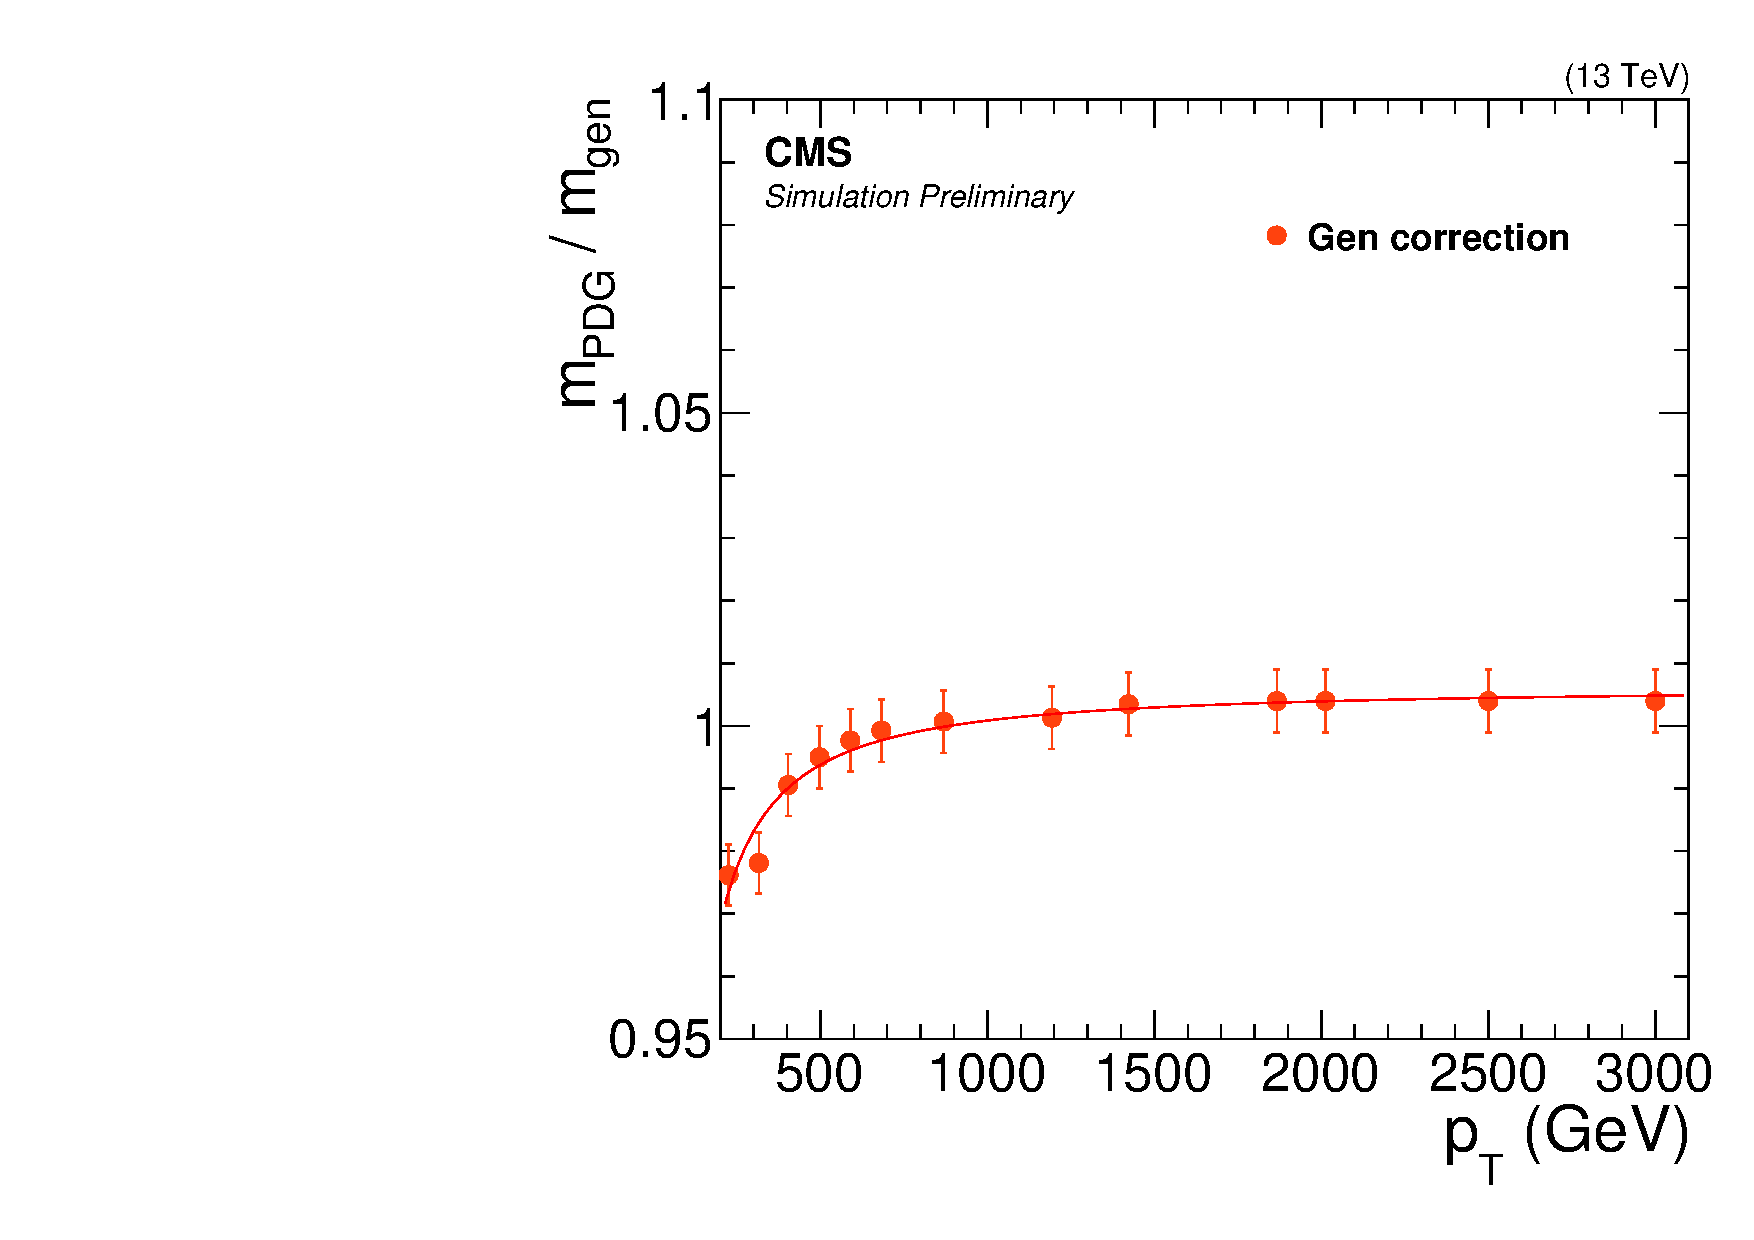
\includegraphics[width=0.45\textwidth]{figures/analysis/search2/AN-16-235/plots/JMC_fit_gen.pdf}
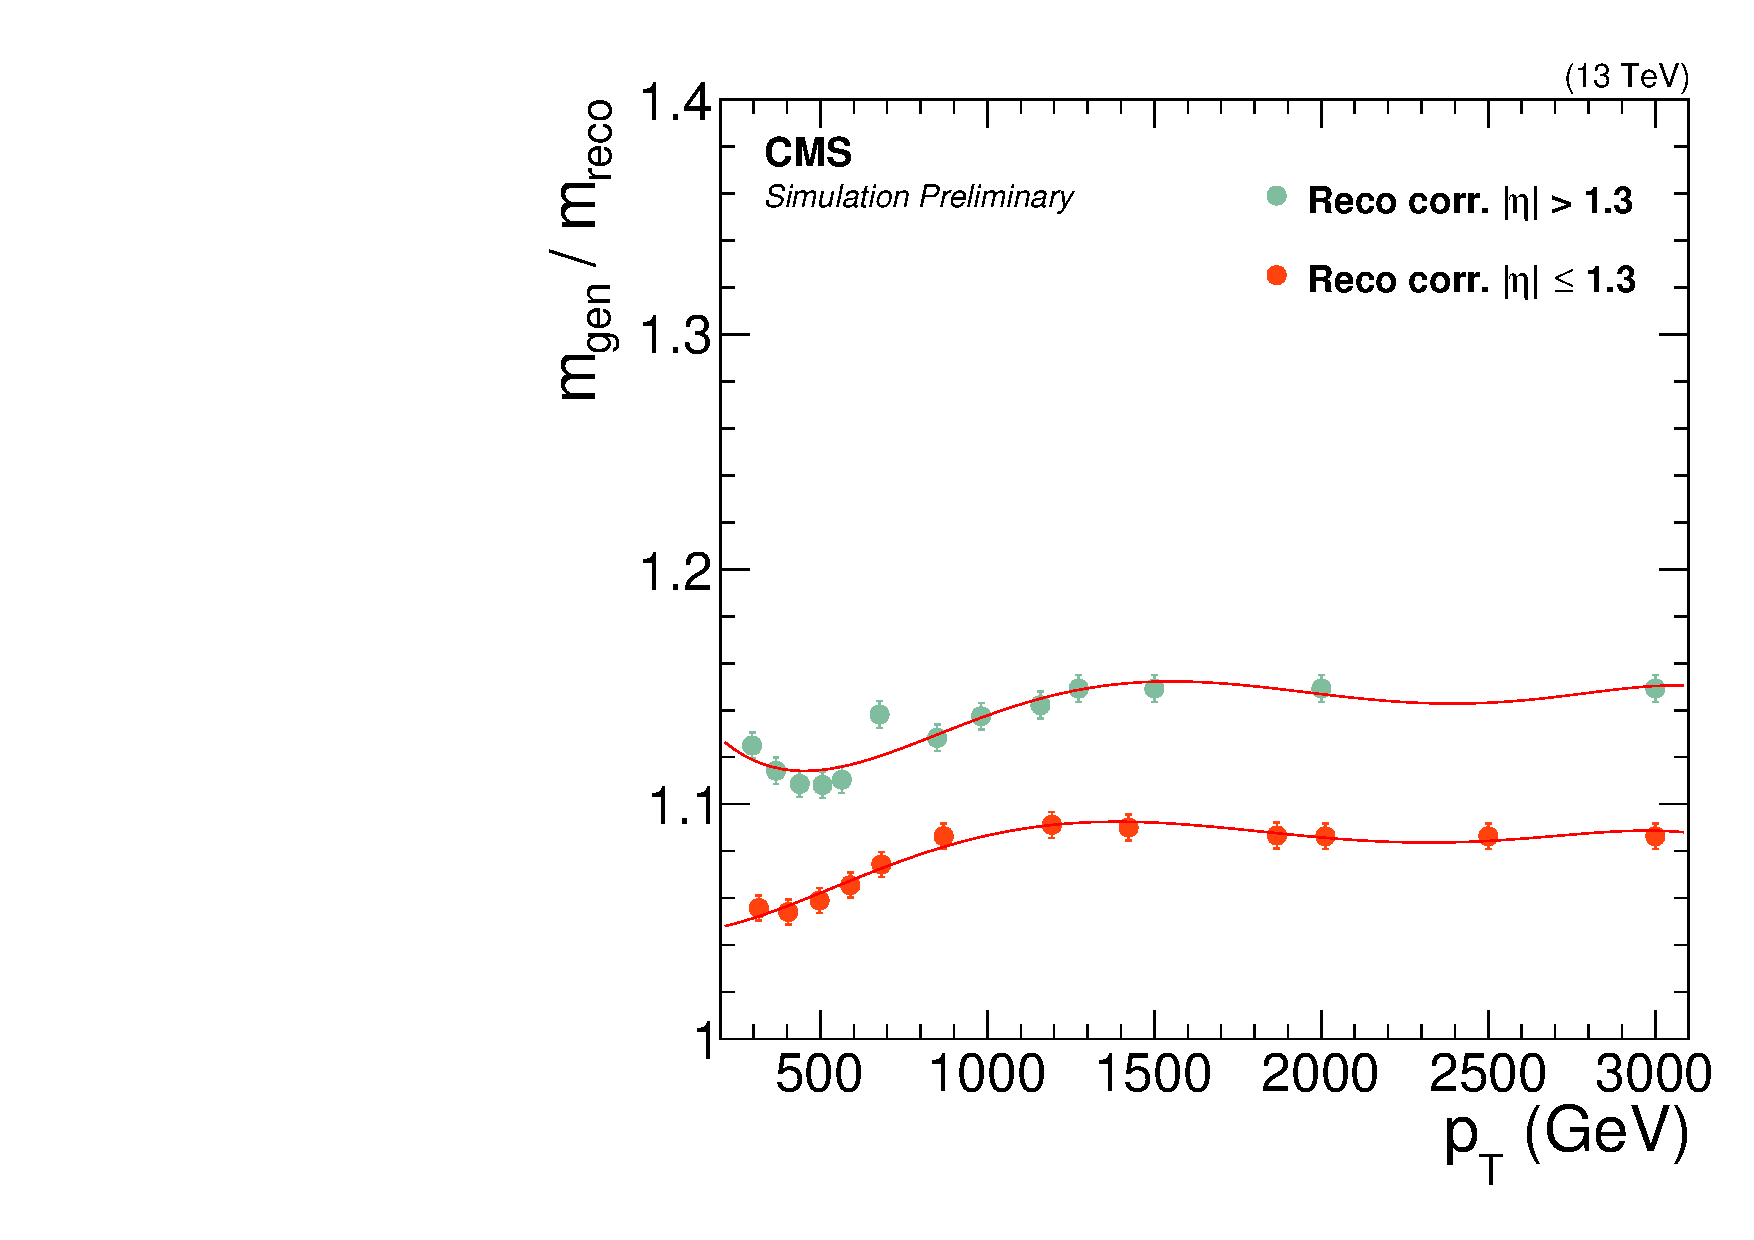
\includegraphics[width=0.45\textwidth]{figures/analysis/search2/AN-16-235/plots/JMC_fit_reco.pdf}
\caption{Fit to $\rm{M_{PDG}/M_{GEN}}$ as a function of jet $\pt$ (left), where $\rm{M_{PDG}}=80.4~\GeV$ and $\rm{M_{GEN}}$ is the fitted mean of the generator level mass and a fit to $\rm{(M_{RECO}-M_{GEN})/M_{RECO}}$ (right), where $\rm{M_{RECO}}$ is the reconstructed softdrop mass, as a function of jet $\pt$ in two $\eta$ bins.}
\label{fig:jmcfits}
\end{figure}
The two corrections are then applied to the uncorrected PUPPI softdrop mass both in data and in MC as
\begin{equation}
M_{SD}=M_{\rm{SD, uncorr}} \times \rm{w_{GEN}} \times \rm{w_{RECO}}
\end{equation}
where $w_{GEN}$ and $w_{RECO}$ correspond to the gen and reco corrections respectively and $M_{\rm{SD, uncorr}}$ is the uncorrected PUPPI softdrop mass. \par
Finally, a closure test is performed in order to check that the corrected PUPPI+softdrop W-jet mass peaks at 80.4 \GeV and is stable with \PT and $\eta$. The fitted mean of the corrected PUPPI softdrop mass peak as a function of jet \PT in two different $\eta$ bins is shown in Figure~\ref{fig:searchII:wtagclosure}. Good closure is observed, with the corrected mass peaking around 80 GeV independent of the jet $\pt$ and $\eta$.The PUPPI softdrop jet mass peak for W/Z-jets from different signal samples after jet mass corrections have been applied is shown in Figure~\ref{fig:search2:corrMass}, for resonances with a mass of 1 and 4 TeV. The corrections applied to Z-jets yield a mass stable with \PT, peaking around the Z mass. 
\begin{figure}[htbp]
\centering
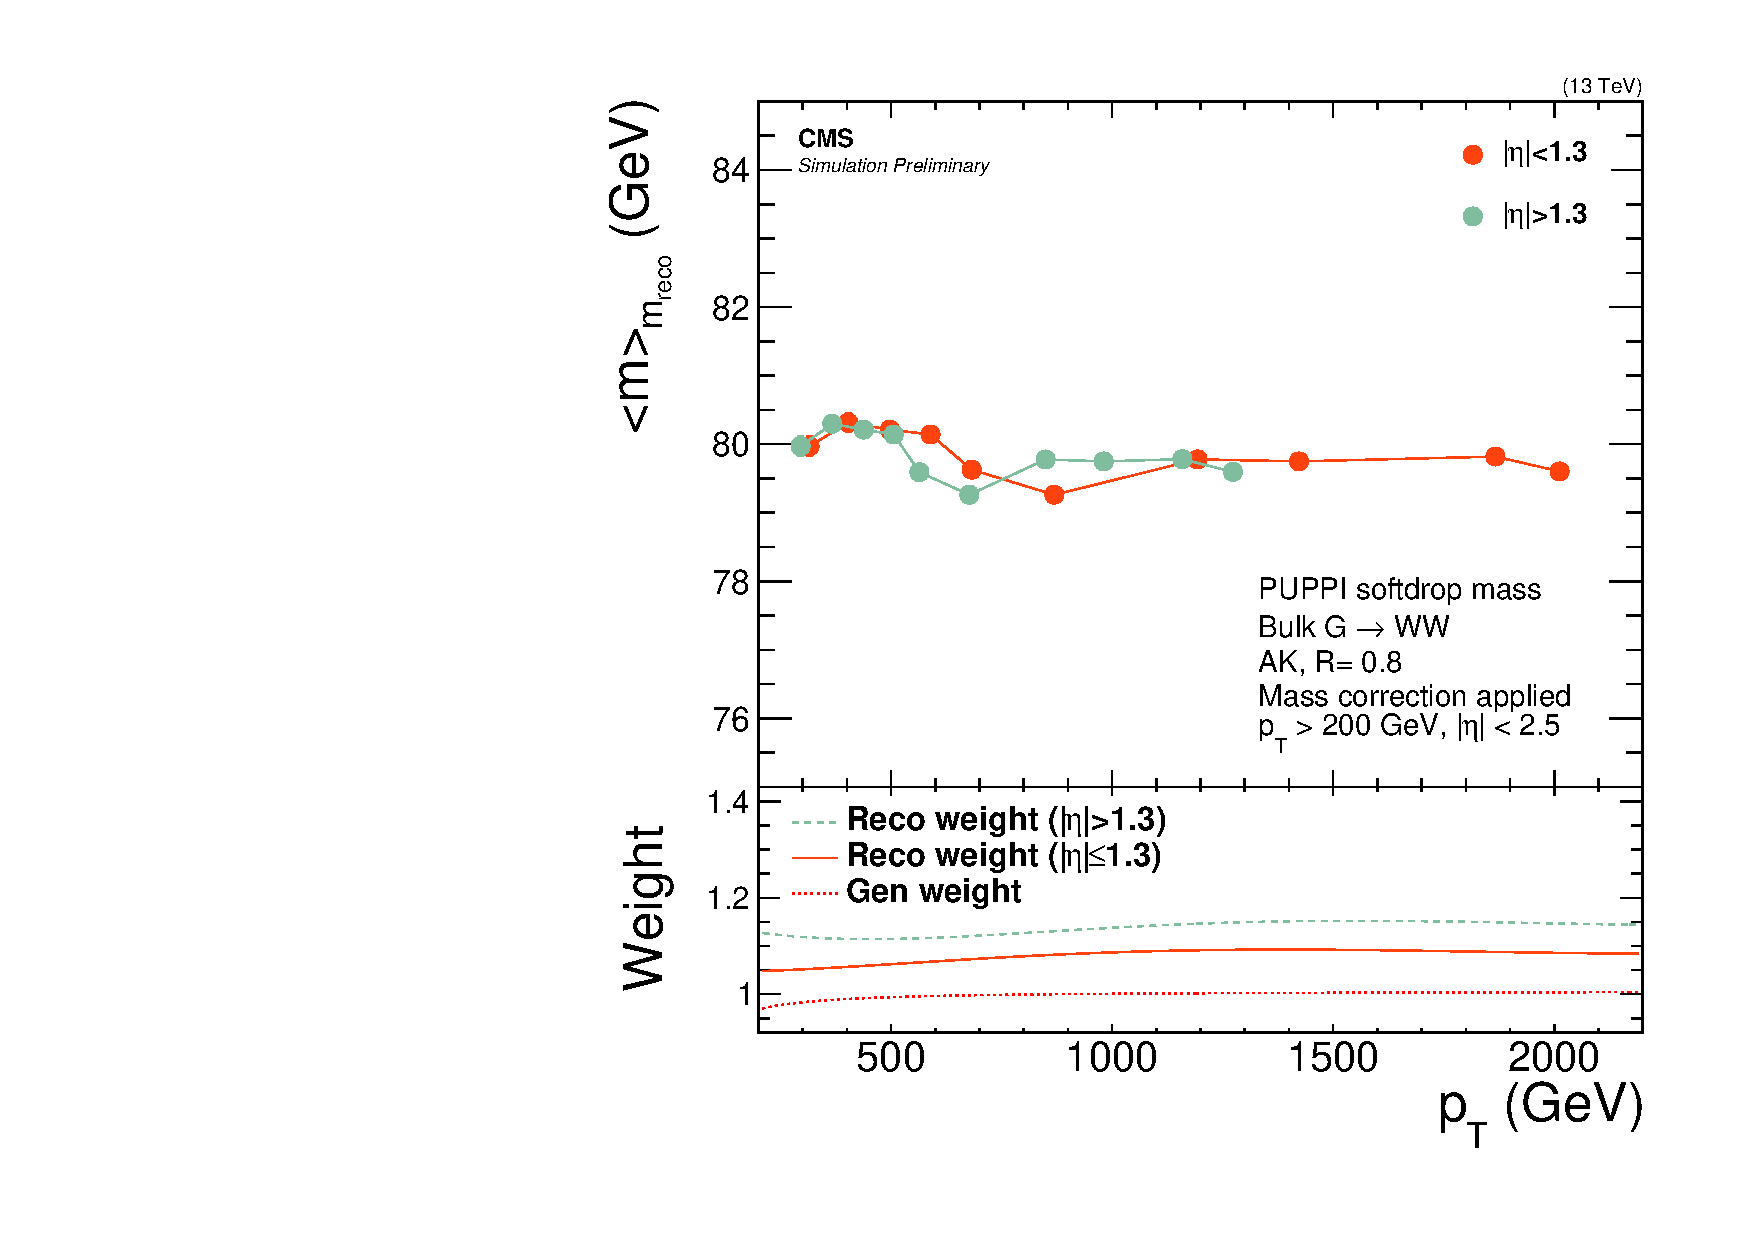
\includegraphics[width=0.49\textwidth]{figures/analysis/search2/AN-16-235/plots/ClosureTest_RecoMass.pdf}
\caption{The mean of the fitted W-jet corrected PUPPI softdrop mass peak as a function of jet $\pt$ in two different $\eta$ bins.}
\label{fig:searchII:wtagclosure}
\end{figure}
\begin{figure}[htbp]
\centering
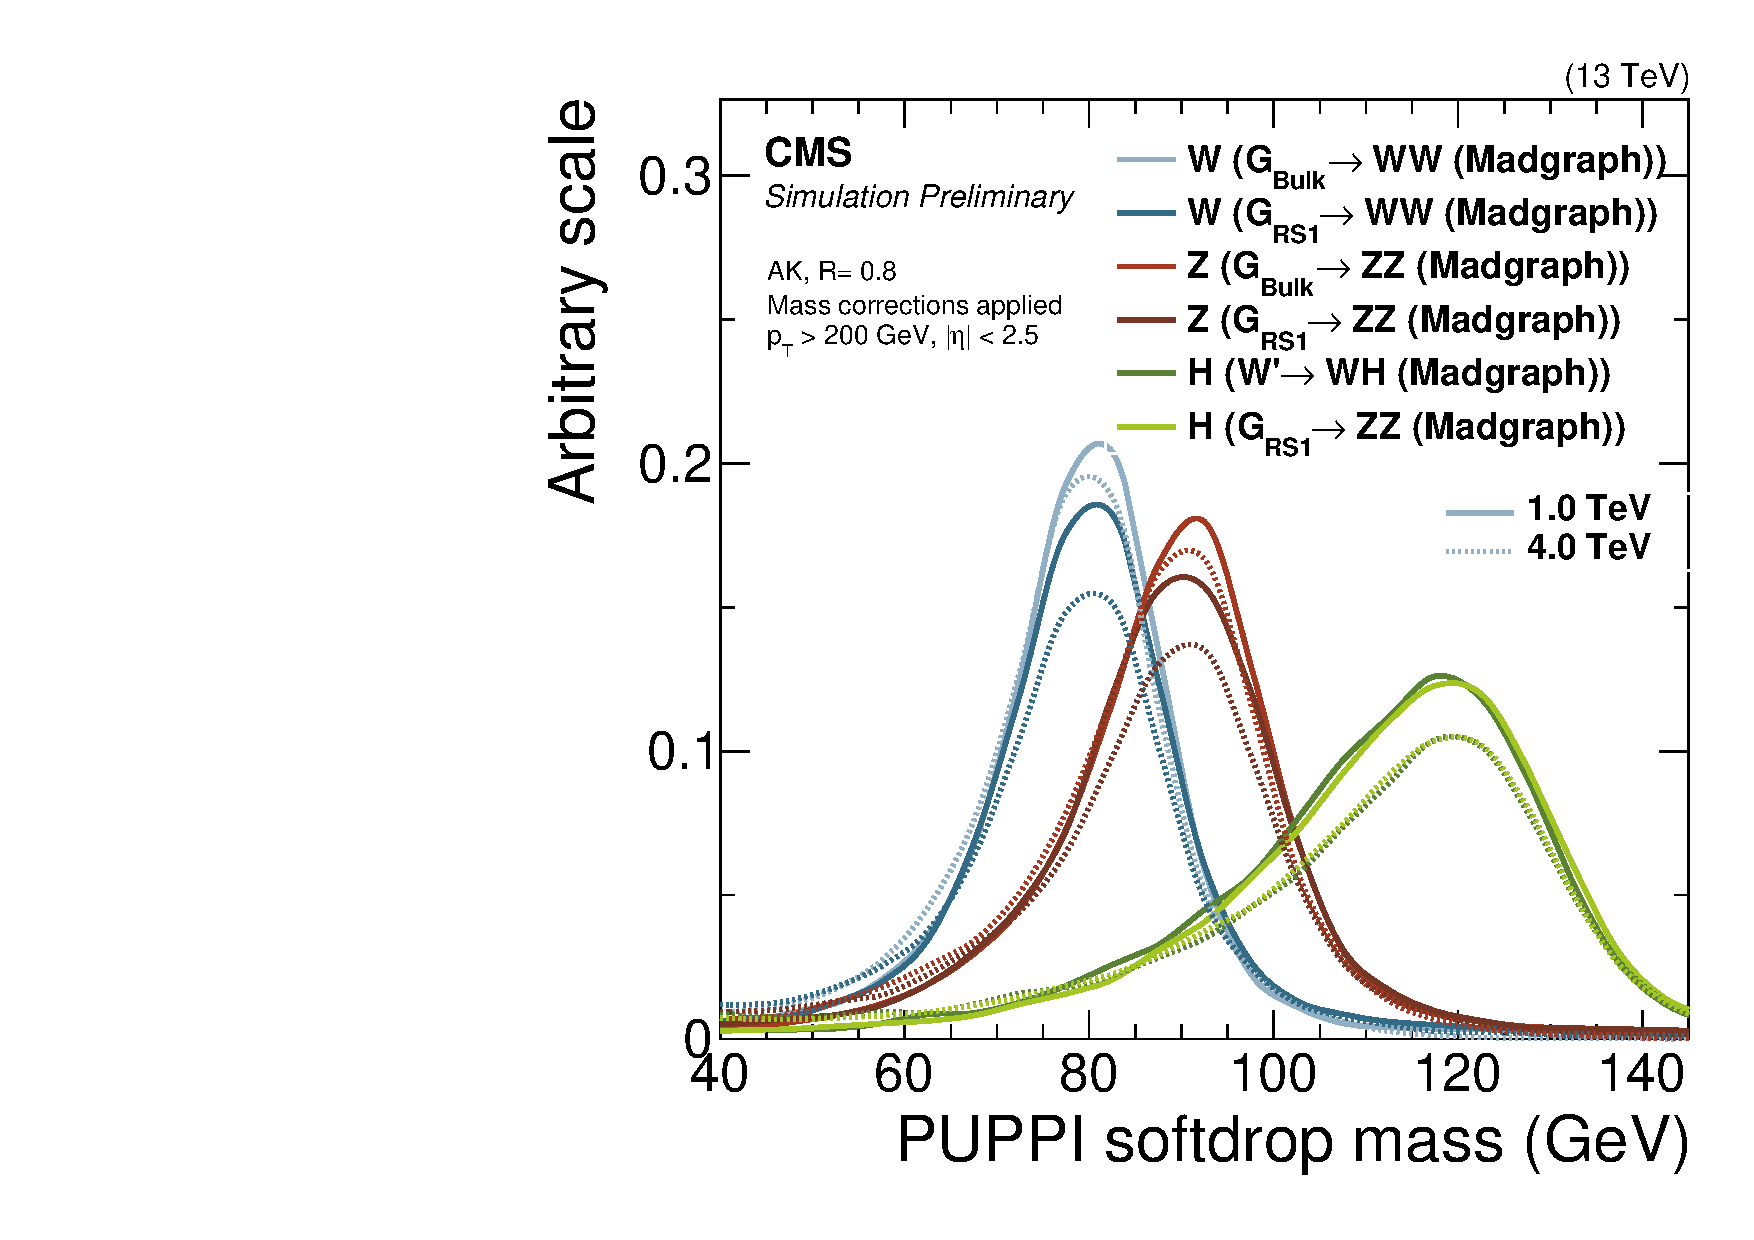
\includegraphics[width=0.49\textwidth]{figures/analysis/search2/AN-16-235/plots/SoftdropMass_NEWCORR_wH0.pdf}
\caption{The W/Z/H-jet corrected PUPPI softdrop mass peak for jets from different signal samples with masses of 1 and 4 TeV.}
\label{fig:search2:corrMass}
\end{figure}

\subsubsection{W-tagging performance}
The new PUPPI+softdrop based \PW/\PZ-tagger uses a mass window of $65 \GeV < m_{SD} < 105 \GeV$ in combination with a cut of PUPPI $\tau_{21}<0.4$.
We compare its performance to that of the CHS+pruning based tagger used in Search I as well as to that of a "DDT-transformed" \nsubj based tagger~\cite{Dolen:2016kst}. The $\tau_{21}^{DDT}$ variable is a linear transformation of \nsubj given as
\begin{equation}
\label{eq:searchII:ddt}
\tau_{21}^{DDT} = \tau_{21} + M \times \log \bigg( \frac{m^2}{p_T \times 1 \textrm{ GeV}}\bigg)
\end{equation}
where $M=-0.063$ is obtained from a fit of $\tau_{21}$ against the variable $\rho^{'}=\log(m^2/\PT/\mu)$, where $\mu = 1 \GeV$.
The purpose of this is to de-correlate $\tau_{21}$ from the softdrop mass and \PT, yielding a mass and dijet invariant mass spectrum minimally sculpted by
a cut on the $\tau_{21}^{DDT}$ tagging variable. This is tagger that will be further explored and explained in detail in the context of Search III, Section~\ref{sec:searchIII:ddt}.\par
The background rejection efficiency for QCD light flavor jets as a function of W-jet signal efficiency is shown in Figure~\ref{fig:searchII:roc}
The efficiency is measured requiring a fixed jet mass window of 65-105 \GeV, while scanning the cut on $\tau_2/\tau_1$.
\begin{figure}[ht!]
\centering
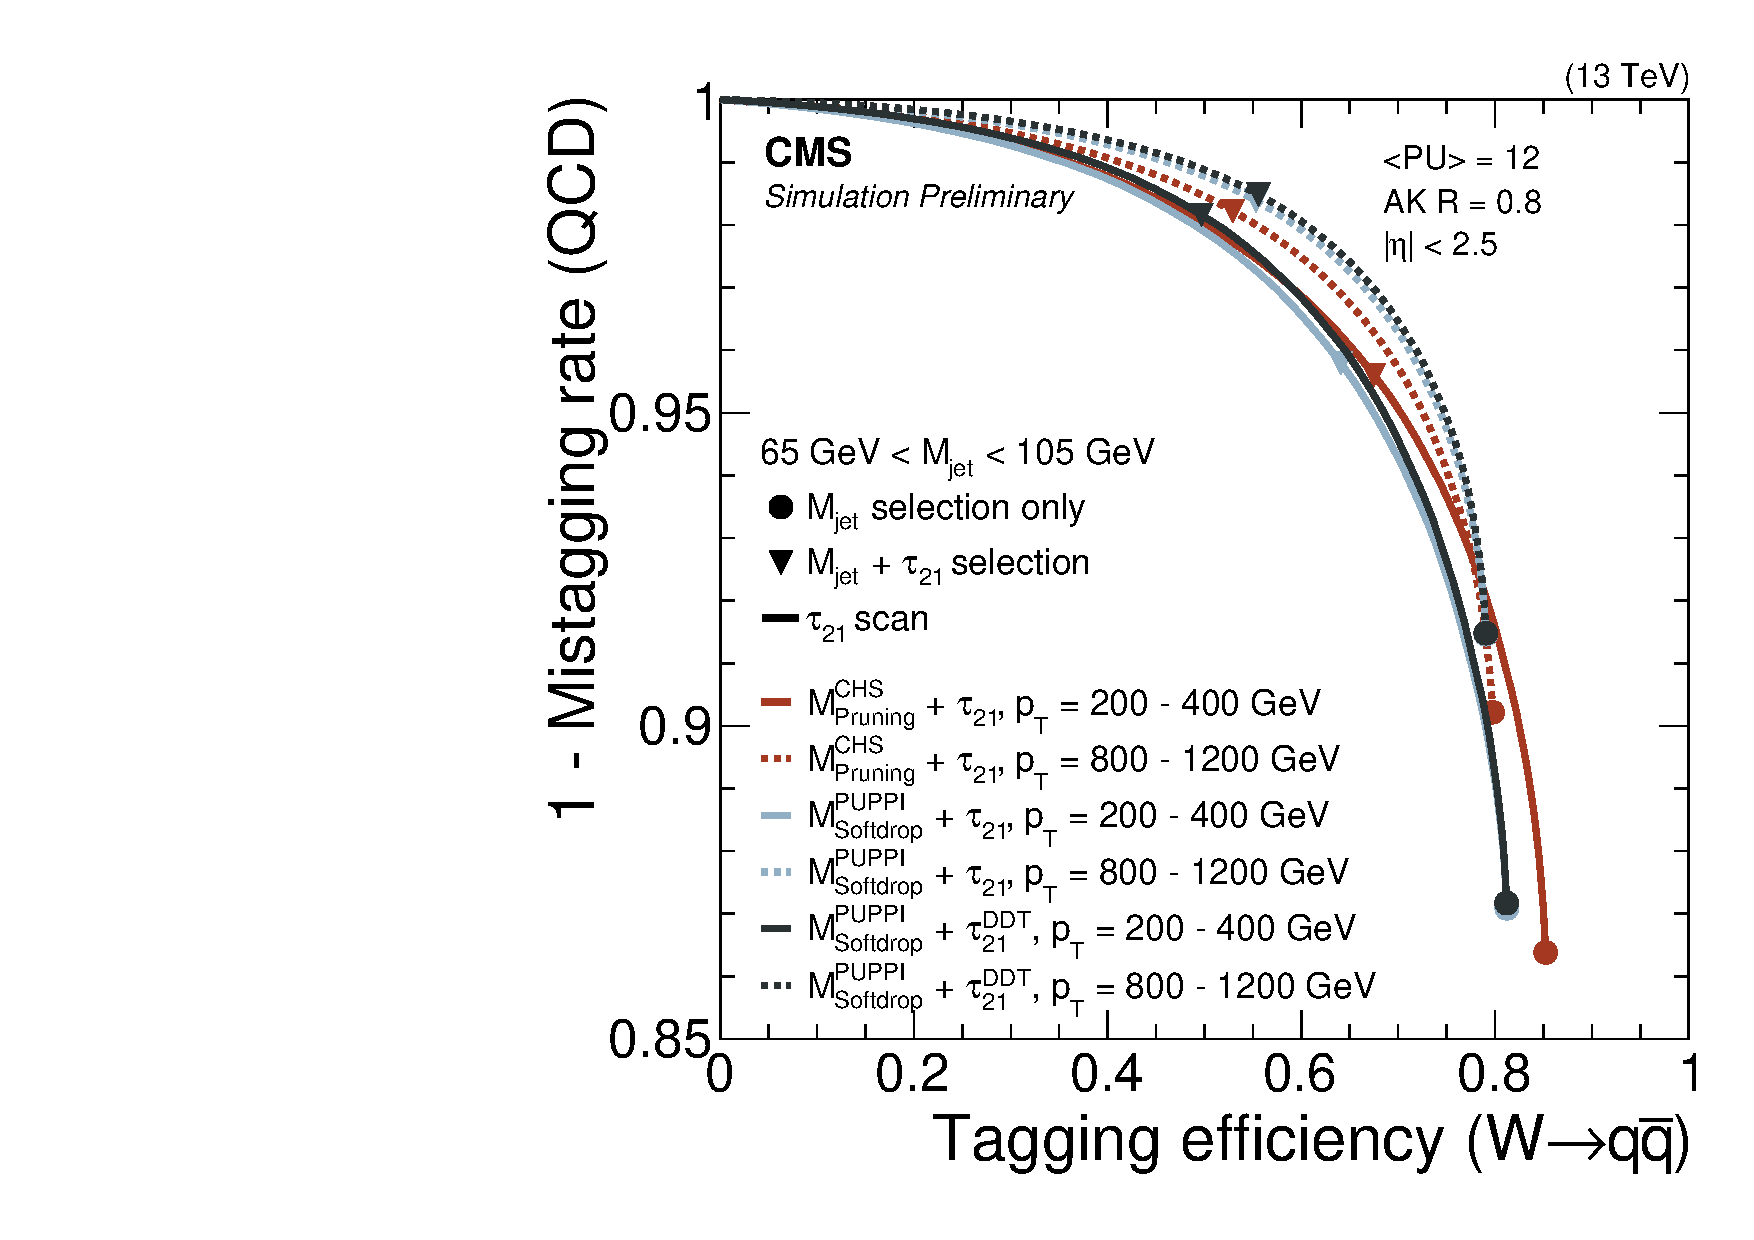
\includegraphics[width=0.49\textwidth]{figures/vtagging/JME-16-003/BoostedW/roc_WqqvsQCD_2bins.pdf}
\caption{The background rejection efficiency for QCD light flavor jets as a function of W-jet signal efficiency. A cut on CHS pruned or PUPPI softdrop jet
mass of $65<m_{\mathrm{jet}}<105$~\GeV is applied while scanning the cut on \nsubj. The cuts corresponding to $\tau_2/\tau_1 < 0.45$ for CHS+pruning, PUPPI $\tau_2/\tau_1 < 0.4$ for PUPPI+softdrop or $\tau_{21}^\text{DDT}<0.52$ are indicated with triangles, while the solid circles represent the efficiency and mistag rate for a mass cut only.}
\label{fig:searchII:roc}
\end{figure}
The general performance of each tagger is very similar, with the PUPPI+softdrop based taggers displaying a slightly higher signal efficiency for a given mistag rate at high \PT and CHS+pruning slightly better at low \PT.
Two better understand the difference between each tagger, we look at the tagging performance as a function of jet \PT as well as pileup, shown in Figure~\ref{fig:searchII:effvspt} and~\ref{fig:searchII:effvspu}.\par
Starting with the tagger \PT-dependence in Figure~\ref{fig:searchII:effvspt}, we observe that she signal efficiency of a PUPPI+softdrop of CHS+pruned jet mass cut is flat as a function of \PT, at around 80\%. The QCD mistagging rate drops for both groomers, with a 1-3\% lower mistag rate using PUPPI+softdrop that CHS+pruning.
\begin{figure}[h!]
\centering
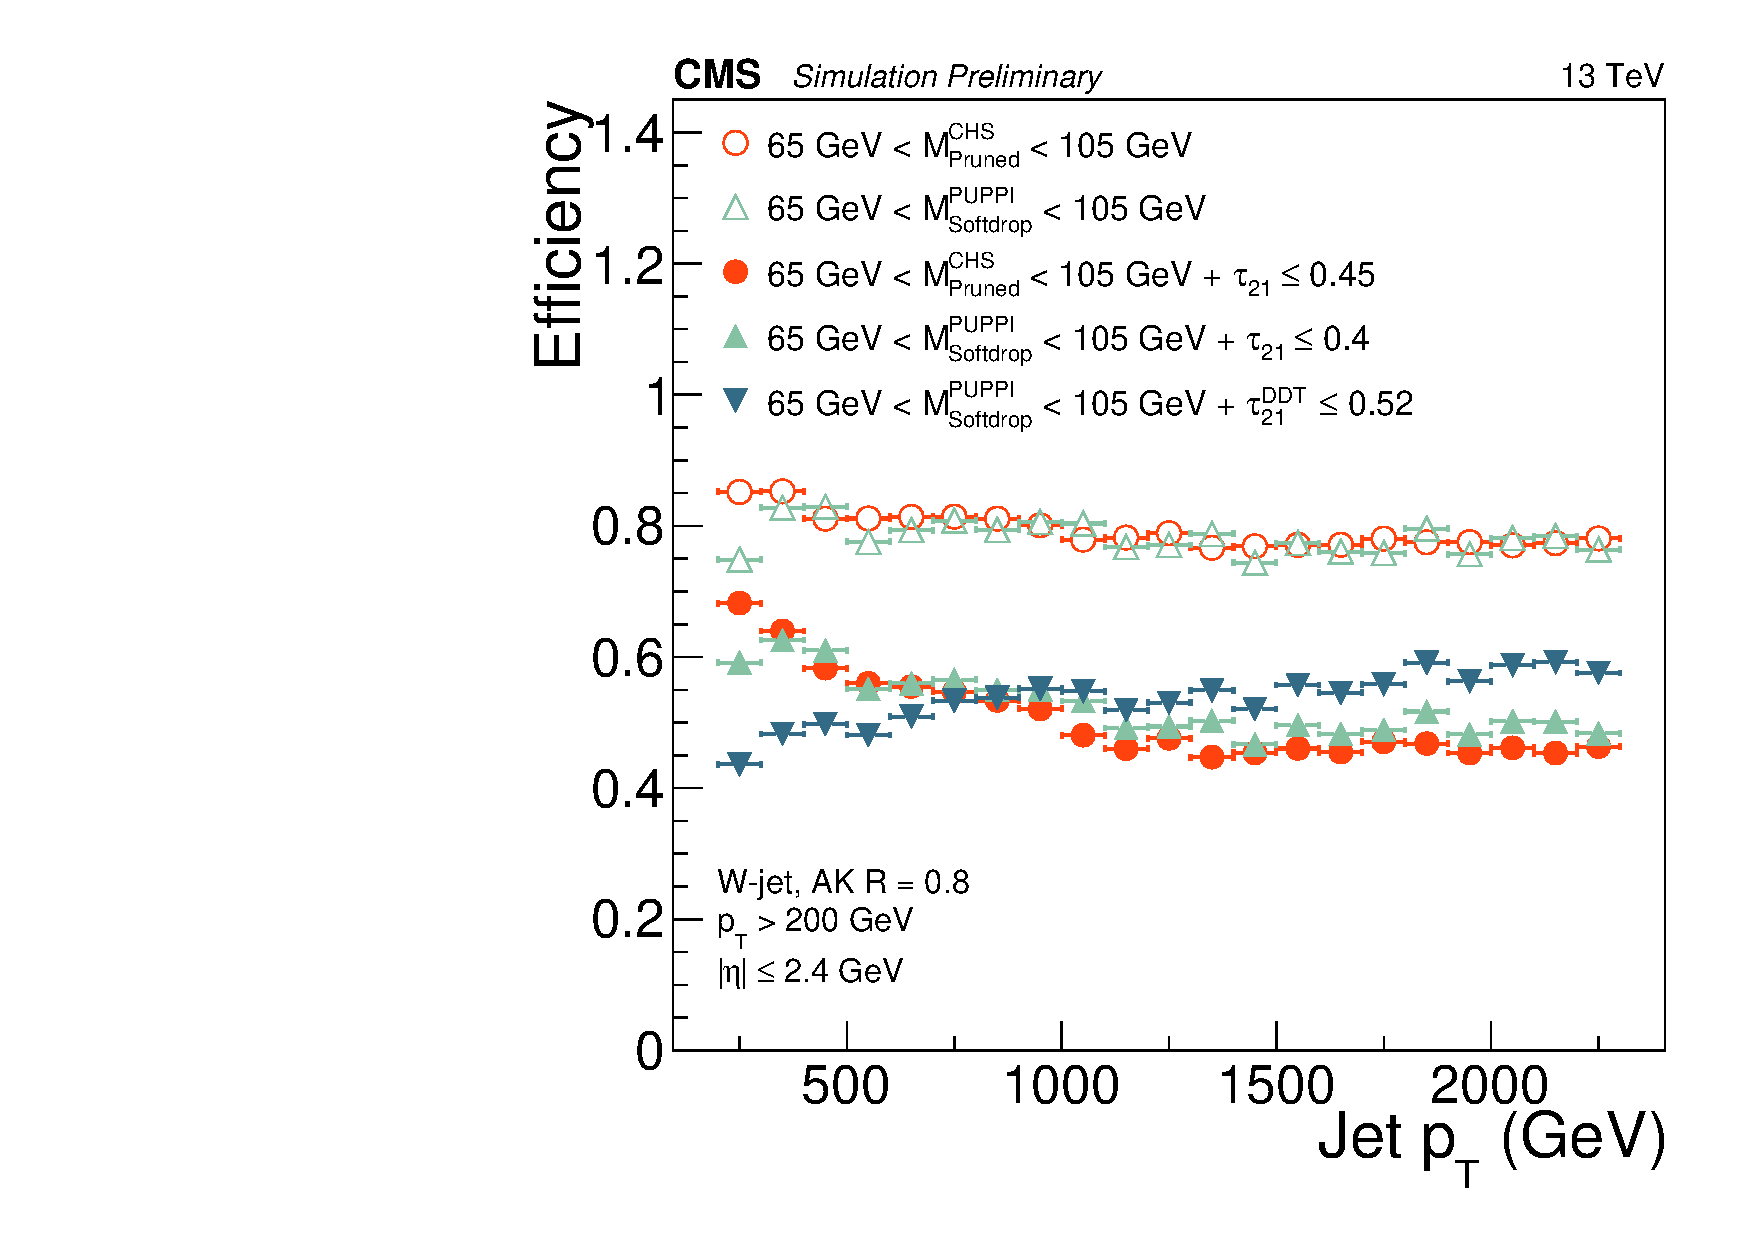
\includegraphics[width=0.49\textwidth]{figures/vtagging/JME-16-003/BoostedW/WtagSigEffvsPT.pdf}
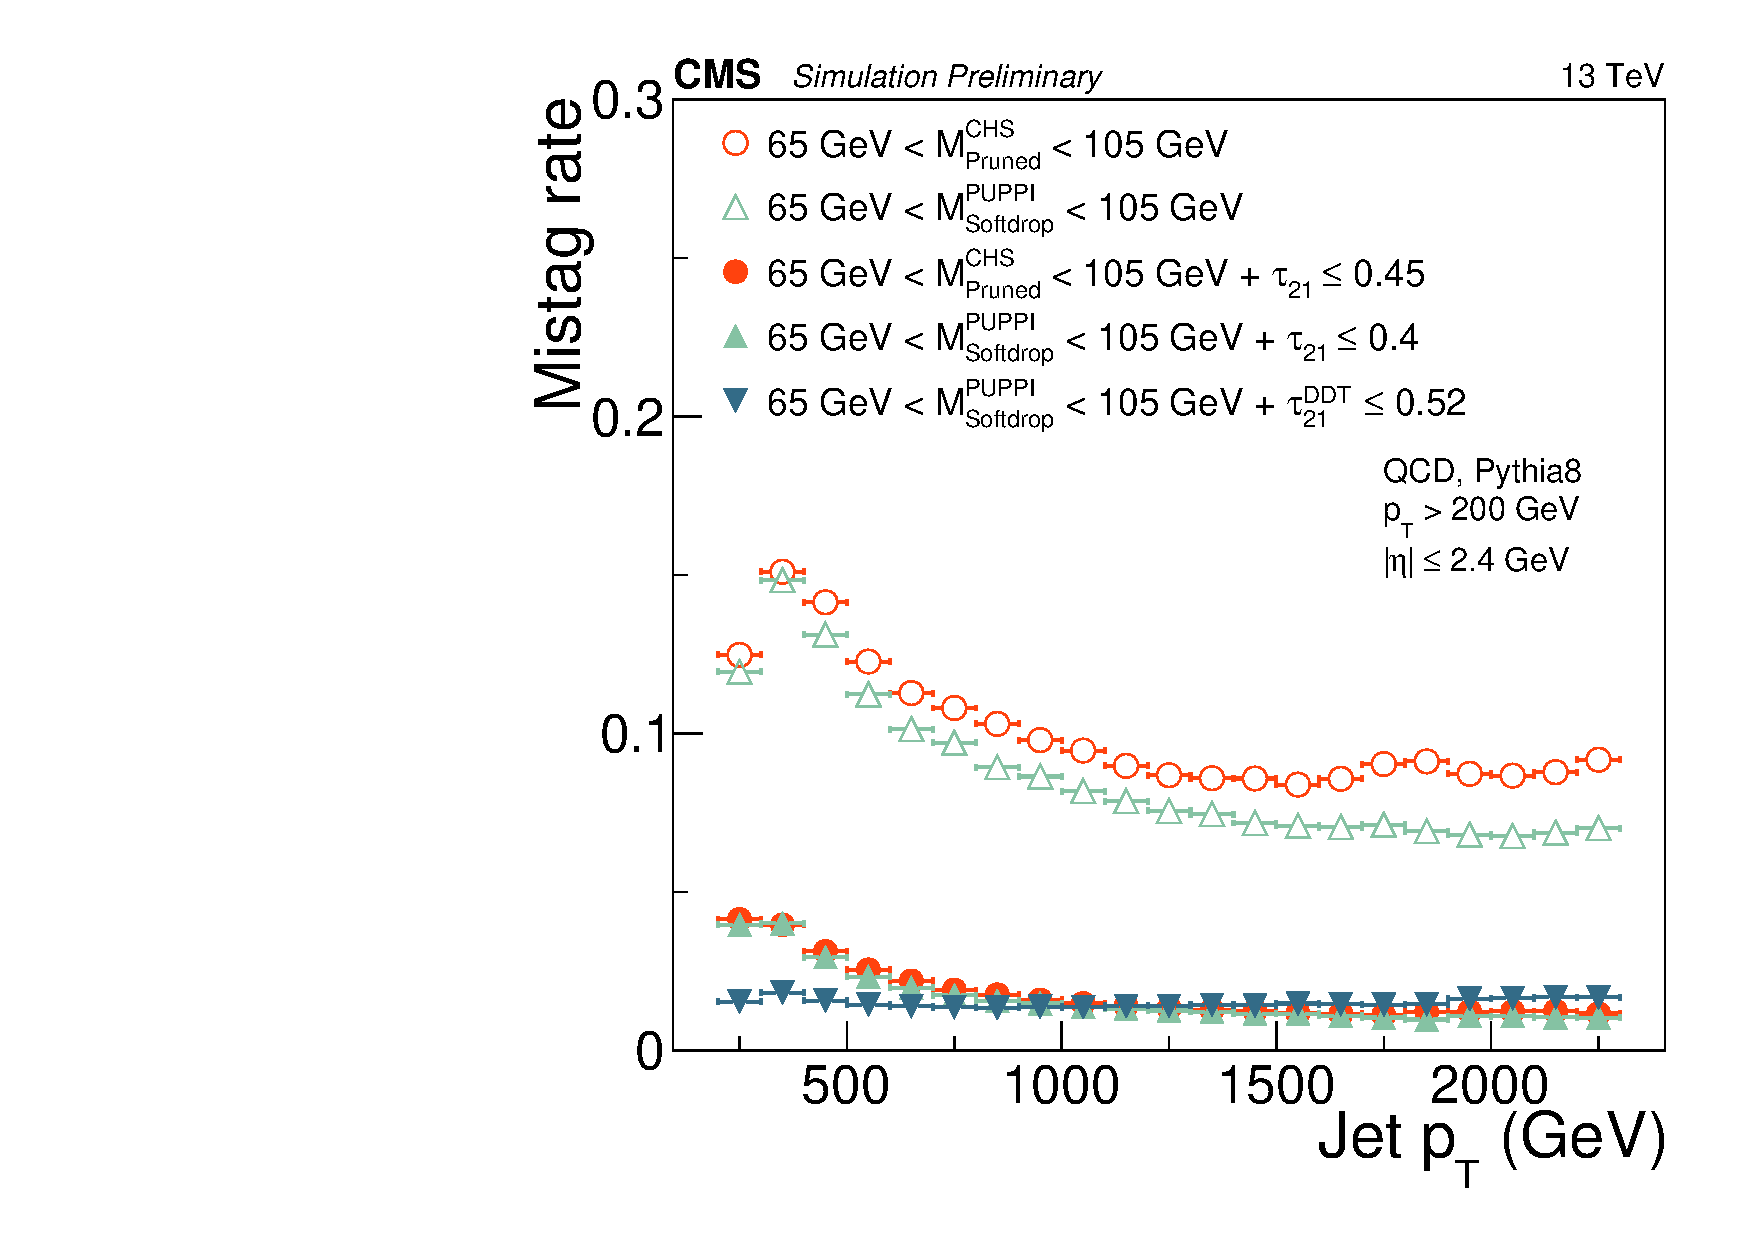
\includegraphics[width=0.49\textwidth]{figures/vtagging/JME-16-003/BoostedW/QCDBkgEffvsPT.pdf}
\caption{W-jet efficiency (left) and QCD light jet mistag rate (right) for a PUPPI+softdrop or CHS+pruned jet mass selection only (hollow circles) and the combined $m_{\mathrm{jet}}$ + (PUPPI) $\tau_2/\tau_1$ (DDT) selection (solid circles) as a function of jet \PT.}
\label{fig:searchII:effvspt}
\end{figure}
Once applying an n-subjettiness cut, the signal efficiency as well as the mistag rate for the PUPPI \nsubj and CHS \nsubj taggers drops as a function of \PT, with an average signal efficiency of around 50\% for a $\sim 2\%$ mistag rate. An interesting behavior is observed for the $\tau_{21}^{DDT}$ tagger: While the mistag rate is flat as a function of \PT, as is the purpose of decorrelated taggers, the signal efficiency improves as the \PT increases, outperforming the other taggers above 1 \TeV. \par
Turning to the tagger pileup dependence, shown in Figure~\ref{fig:searchII:effvspu}, the expected benefit from using the PUPPI algorithm is observed: The tagging efficiency for the CHS+pruning (red solid cirles) based tagger falls of steeply versus the number of primary vertices in the event, while the PUPPI+softdrop based taggers (light and dark blue solid circles) are more or less insensitive to pileup.
\begin{figure}[h!]
\centering
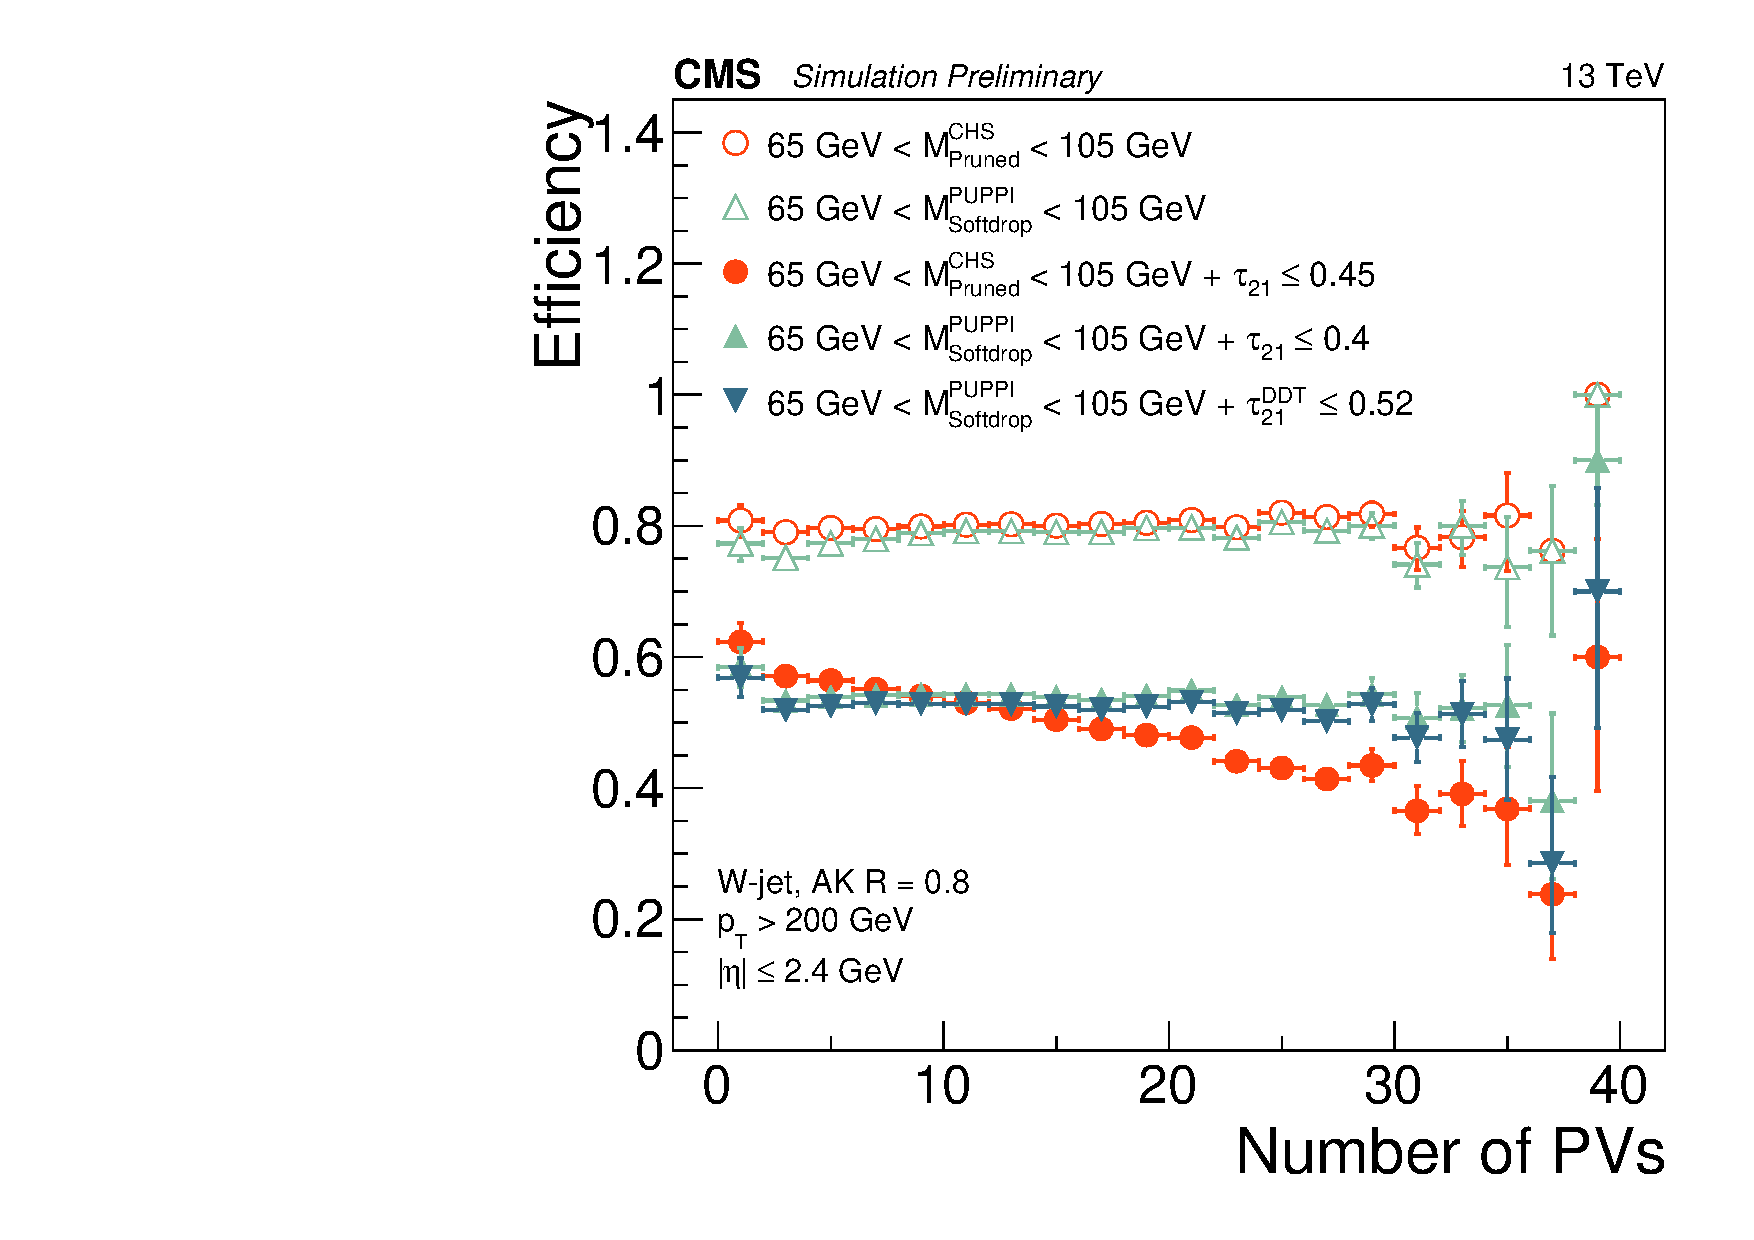
\includegraphics[width=0.49\textwidth]{figures/vtagging/JME-16-003/BoostedW/WtagSigEffvsNPV.pdf}
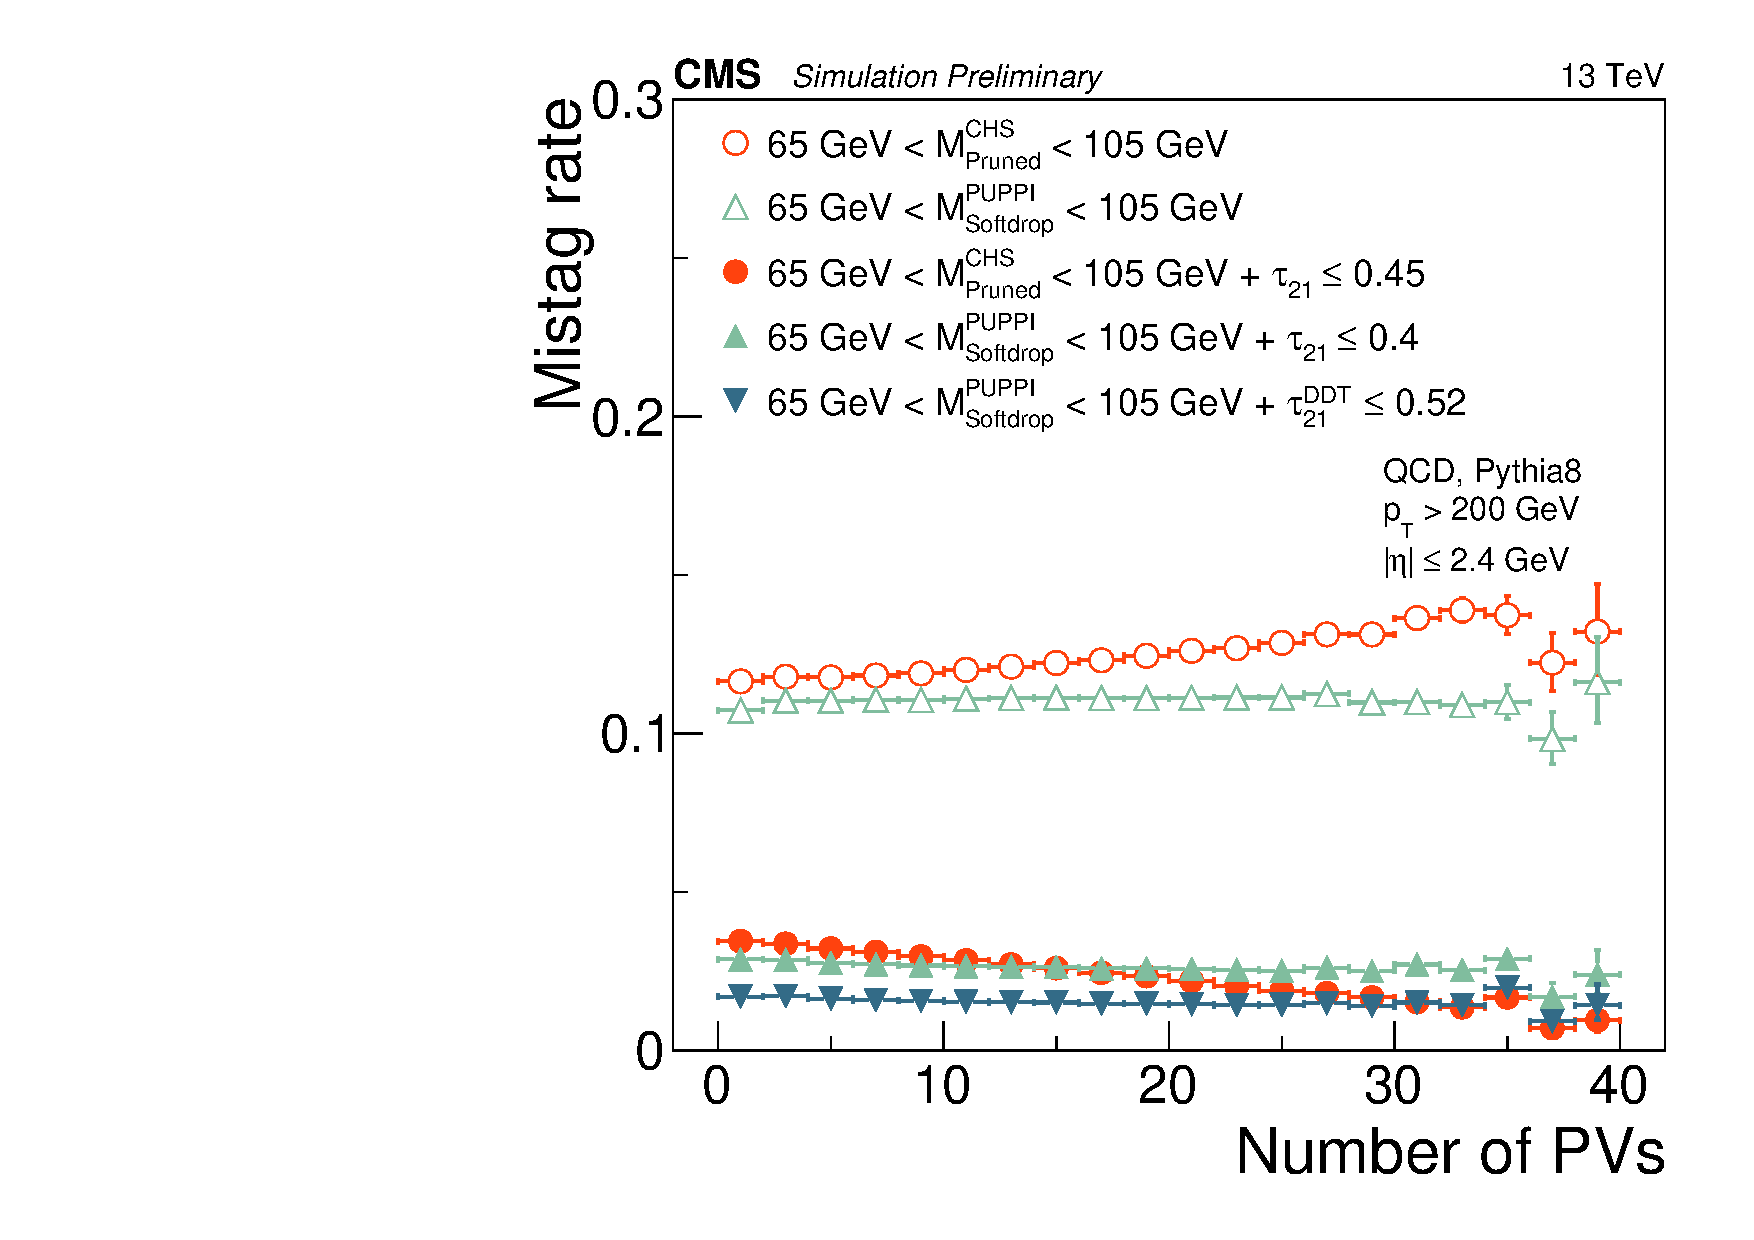
\includegraphics[width=0.49\textwidth]{figures/vtagging/JME-16-003/BoostedW/QCDBkgEffvsNPV.pdf}
\caption{W-jet efficiency (left) and QCD light jet mistag rate (right) for a PUPPI+softdrop or CHS+pruned jet mass selection only (hollow circles) and the combined $m_{\mathrm{jet}}$ + (PUPPI) $\tau_2/\tau_1$ (DDT) selection (solid circles) as a function of jet pileup.}
\label{fig:searchII:effvspu}
\end{figure}
Based on general performance, tagging stability versus pileup and due to theoretical considerations, PUPPI sofdrop mass with dedicated mass corrections applied together with PUPPI \nsubj is chosen as this analysis W-tagger. The per-jet efficiency is around 50-55\% for a 1-2\% mistag rate.\par

\subsubsection{Efficiency scale factors and mass scale/resolution measurement} 
\label{sec:searchII:wtagsf}
subsubsection{Efficiency scale factors and mass scale/resolution measurement} 
\label{sec:searchII:wtagsf}
In order to measure the W-tagging efficiency, jet mass scale and resolution for the new PUPPI+softdrop based tagger, we use the same procedure as outlined in Section~\ref{sec:searchI:vtag}. We first did an early measurement of the efficiency using 2.3 \fbinv of data collected in 2015, which was published in a jet algorithms performance note~\cite{CMS-PAS-JME-16-003} and served as the first commissioning of the new tagger. We then redid the measurement with 12.9 and 35.9 \fbinv of 2016 data, respectively, for the two analyses presented in this chapter (the latter measurement performed by a separate analysis team). The results shown in the following will be those obtained during the commissioning of the tagger, while those used in the two analyses are listed in Appendix~\ref{app:sf16}.
In order to better understand the differences between the CHS+pruning and PUPPI+softdrop based taggers, the first efficiency measurement was done in parallel for both algorithms, requiring either a softdrop or a pruned jet mass between 40 \GeV and 150 \GeV. The softdrop mass is computed after PUPPI and the jet mass corrections as described in Section~\ref{sec:searchII:masscorr} are applied, while the pruned mass is corrected with L2L3 jet energy corrections. 
The method is the same as the one outlined in detail in Section~\ref{sec:searchI:vtag} and fits to matched \ttbar MC and minor backgrounds for the PUPPI softdrop based tagger are skipped here and can be found in Appendix~\ref{app:sf16}.\newline
The PUPPI softdrop jet mass and PUPPI $\tau_{21}$ variables in data and in MC are shown in Figure~\ref{fig:searchII:ttbarcp} and can be compared to the corresponding plots for the CHS pruned jet mass and CHS \nsubj distributions in Figure~\ref{fig:searchII:ttbarcp}. The data to MC agreement as well as the observed spectra, is very similar between CHS pruning and PUPPI softdrop in this region.

\begin{figure}[ht!]
\centering
\begin{tabular}{cc}
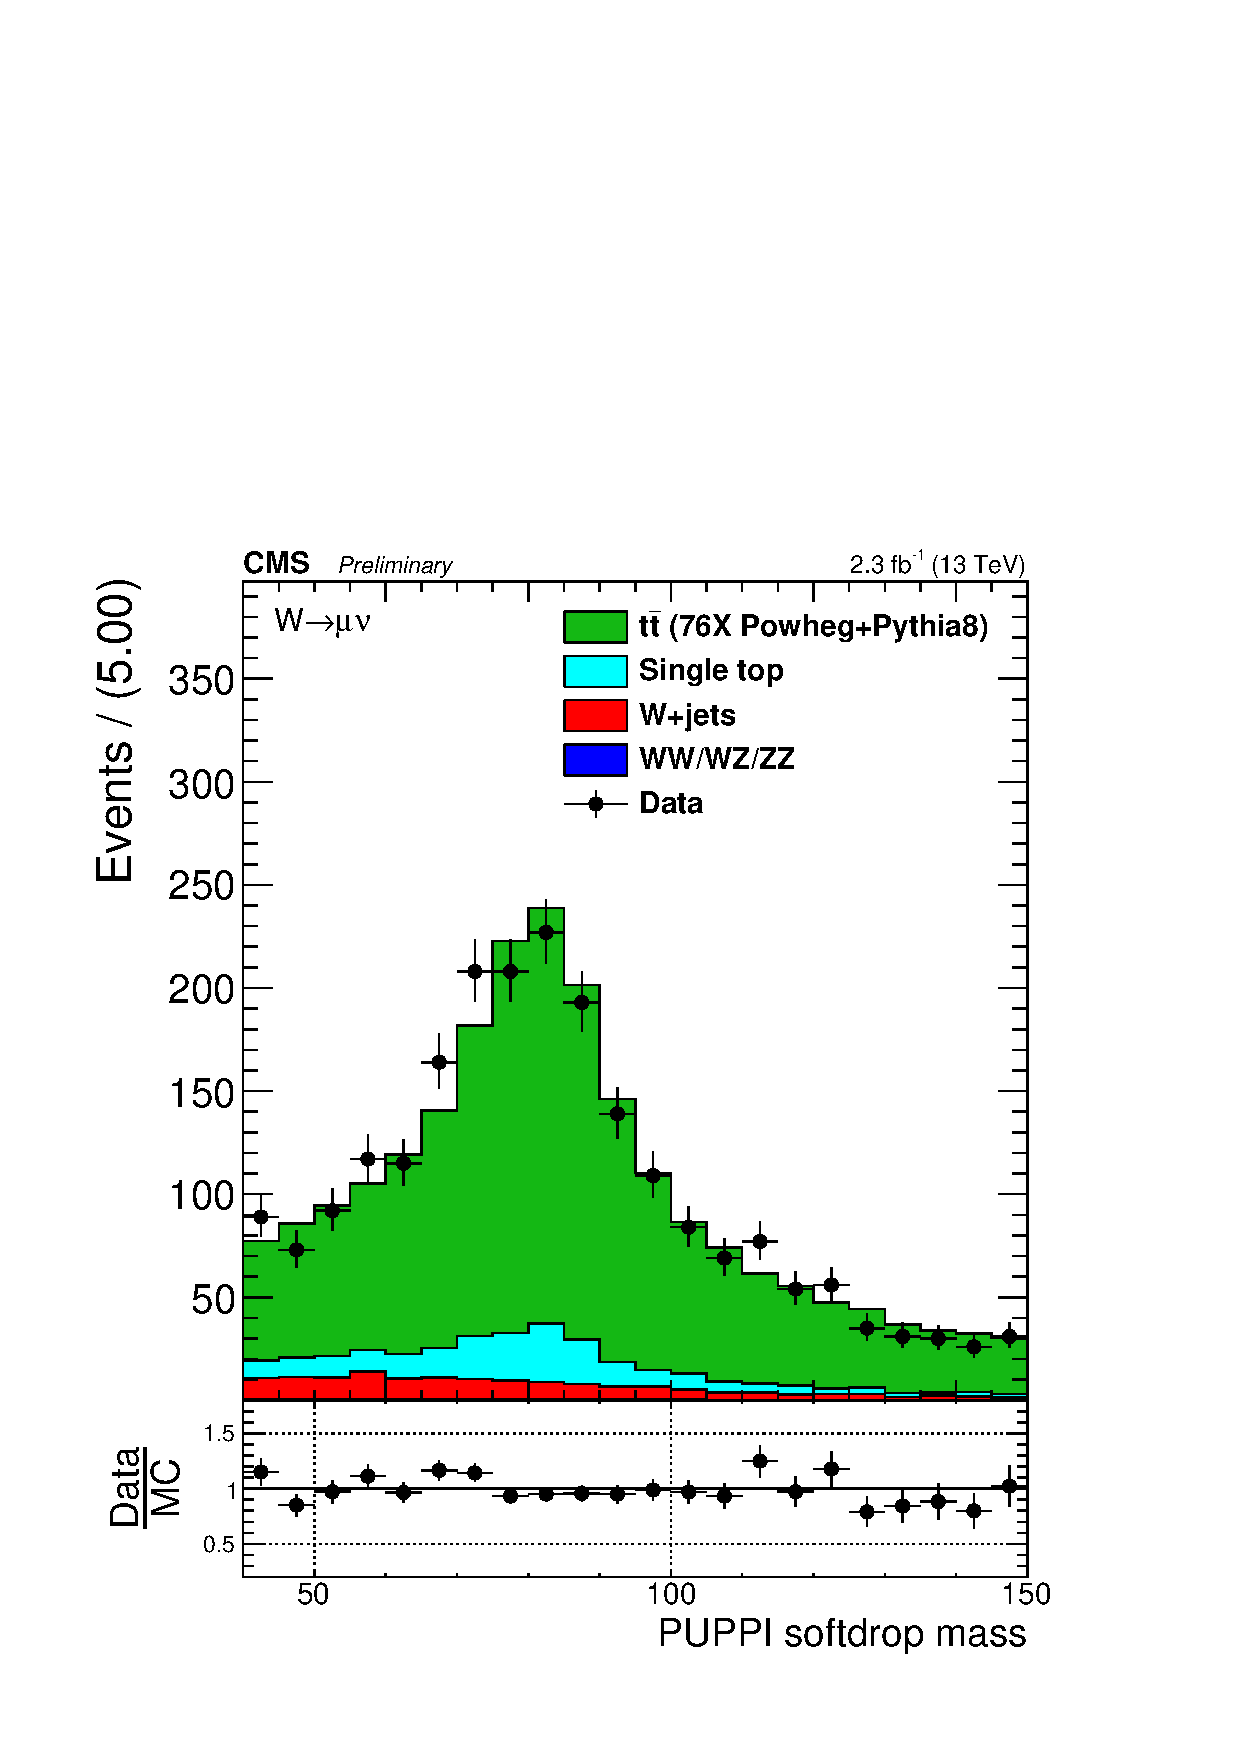
\includegraphics[width=0.5\textwidth]{figures/vtagging/AN-16-215/Whadr_puppi_softdrop_mu.pdf}
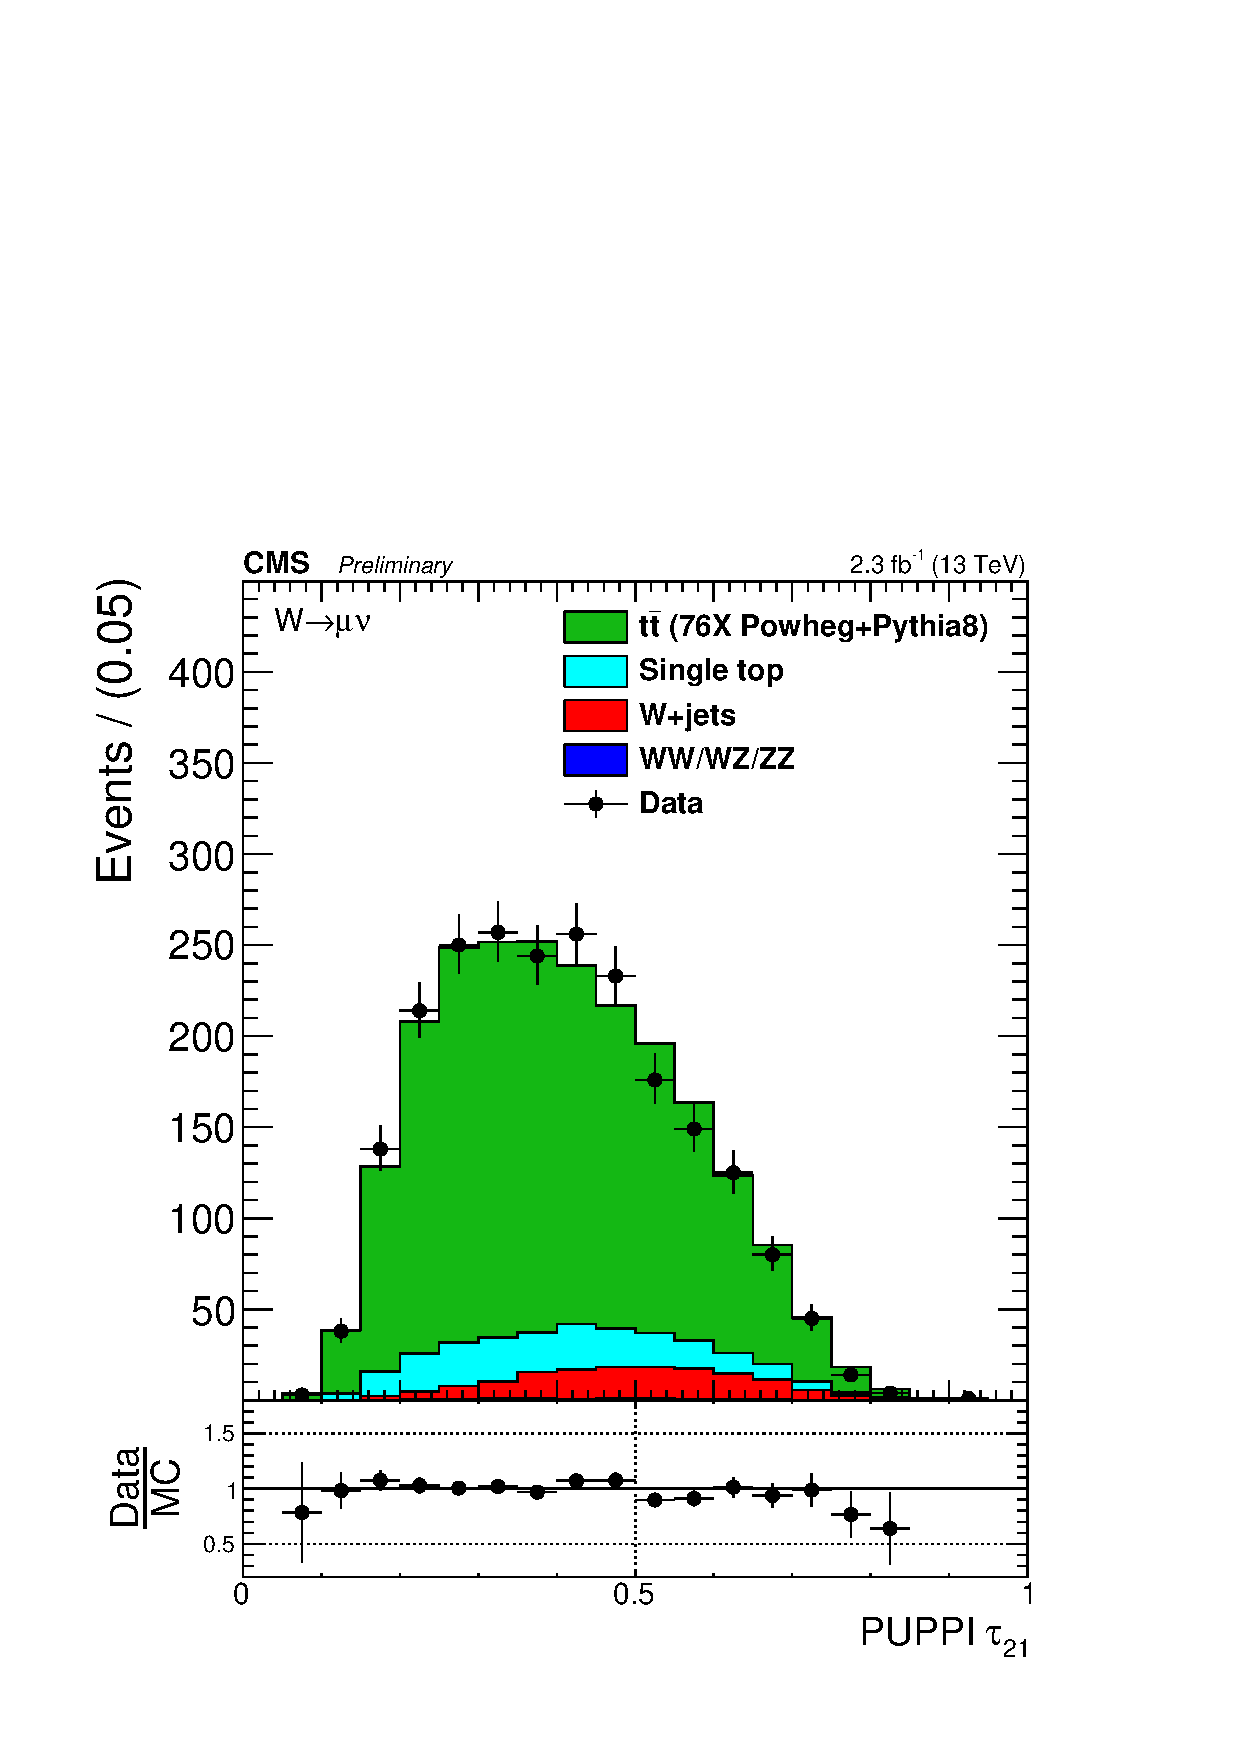
\includegraphics[width=0.5\textwidth]{figures/vtagging/AN-16-215/Whadr_puppi_tau2tau1_mu.pdf}\\
\end{tabular}
\caption{Distribution of the PUPPI softdrop mass (left) and PUPPI n-subjettiness (right) distribution in the \ttbar control sample.}
\label{fig:searchII:ttbarcp}
\end{figure}

Following what was done in Section~\ref{sec:searchI:vtag}, we extract and compare the W-tagging efficiency, jet mass scale and resolution of the combined jet mass and \nsubj selection in data and in MC. This is done through a simultaneous fit of the the softdrop jet mass spectrum between 40 and 150 \GeV in two regions:
\begin{itemize}
\itemsep0em
  \item Pass region: $0 <  \nsubj \leq 0.40$ $\sim$ high purity
  \item Fail region: $0.40 < \nsubj \leq 0.75$ $\sim$ low purity
\end{itemize}
The corresponding fits are shown in Figure~\ref{fig:searchII:simfit}, with the corresponding extracted efficiencies from the Gaussian component of the total fit and scale factors summarized in Table~\ref{tab:searchII:WtagSFs}.
The quoted systematic uncertainties are evaluated the same was as described in Section~\ref{sec:searchI:wtagsystematic} and correspond to the uncertainty due to ME generator and due to choice of fit method.
\begin{table}[h!]
   \centering
   \footnotesize
   \begin{tabular}{|l|l|c|c|c|}
   \hline
   Category & Working point & Eff. data & Eff. simulation & Scale factor\\
   \hline
   HP& $\tau_2 / \tau_1 < 0.4$         & $0.785 \pm 0.045 $& $0.81 \pm 0.01$   &$0.97 \pm 0.06~\rm{(stat)} \pm 0.04~\rm{(sys)} \pm 0.06~\rm{(sys)}$\\
   LP& $0.45 < \tau_2 / \tau_1 < 0.75$ & $0.215 \pm 0.057 $& $0.204 \pm 0.041$ &$1.13 \pm 0.24~\rm{(stat)} \pm 0.17~\rm{(sys)}  \pm 0.12~\rm{(sys)}$\\
   \hline
   \end{tabular}
   \caption{W-tagging scale factors for both categories the high purity and low purity categories for two taggers: Pruned jet mass + \nsubj and PUPPI softdrop jet mass + PUPPI \nsubj. }
   \label{tab:searchII:WtagSFs}
\end{table}


\begin{figure}[htbp]
\centering
% 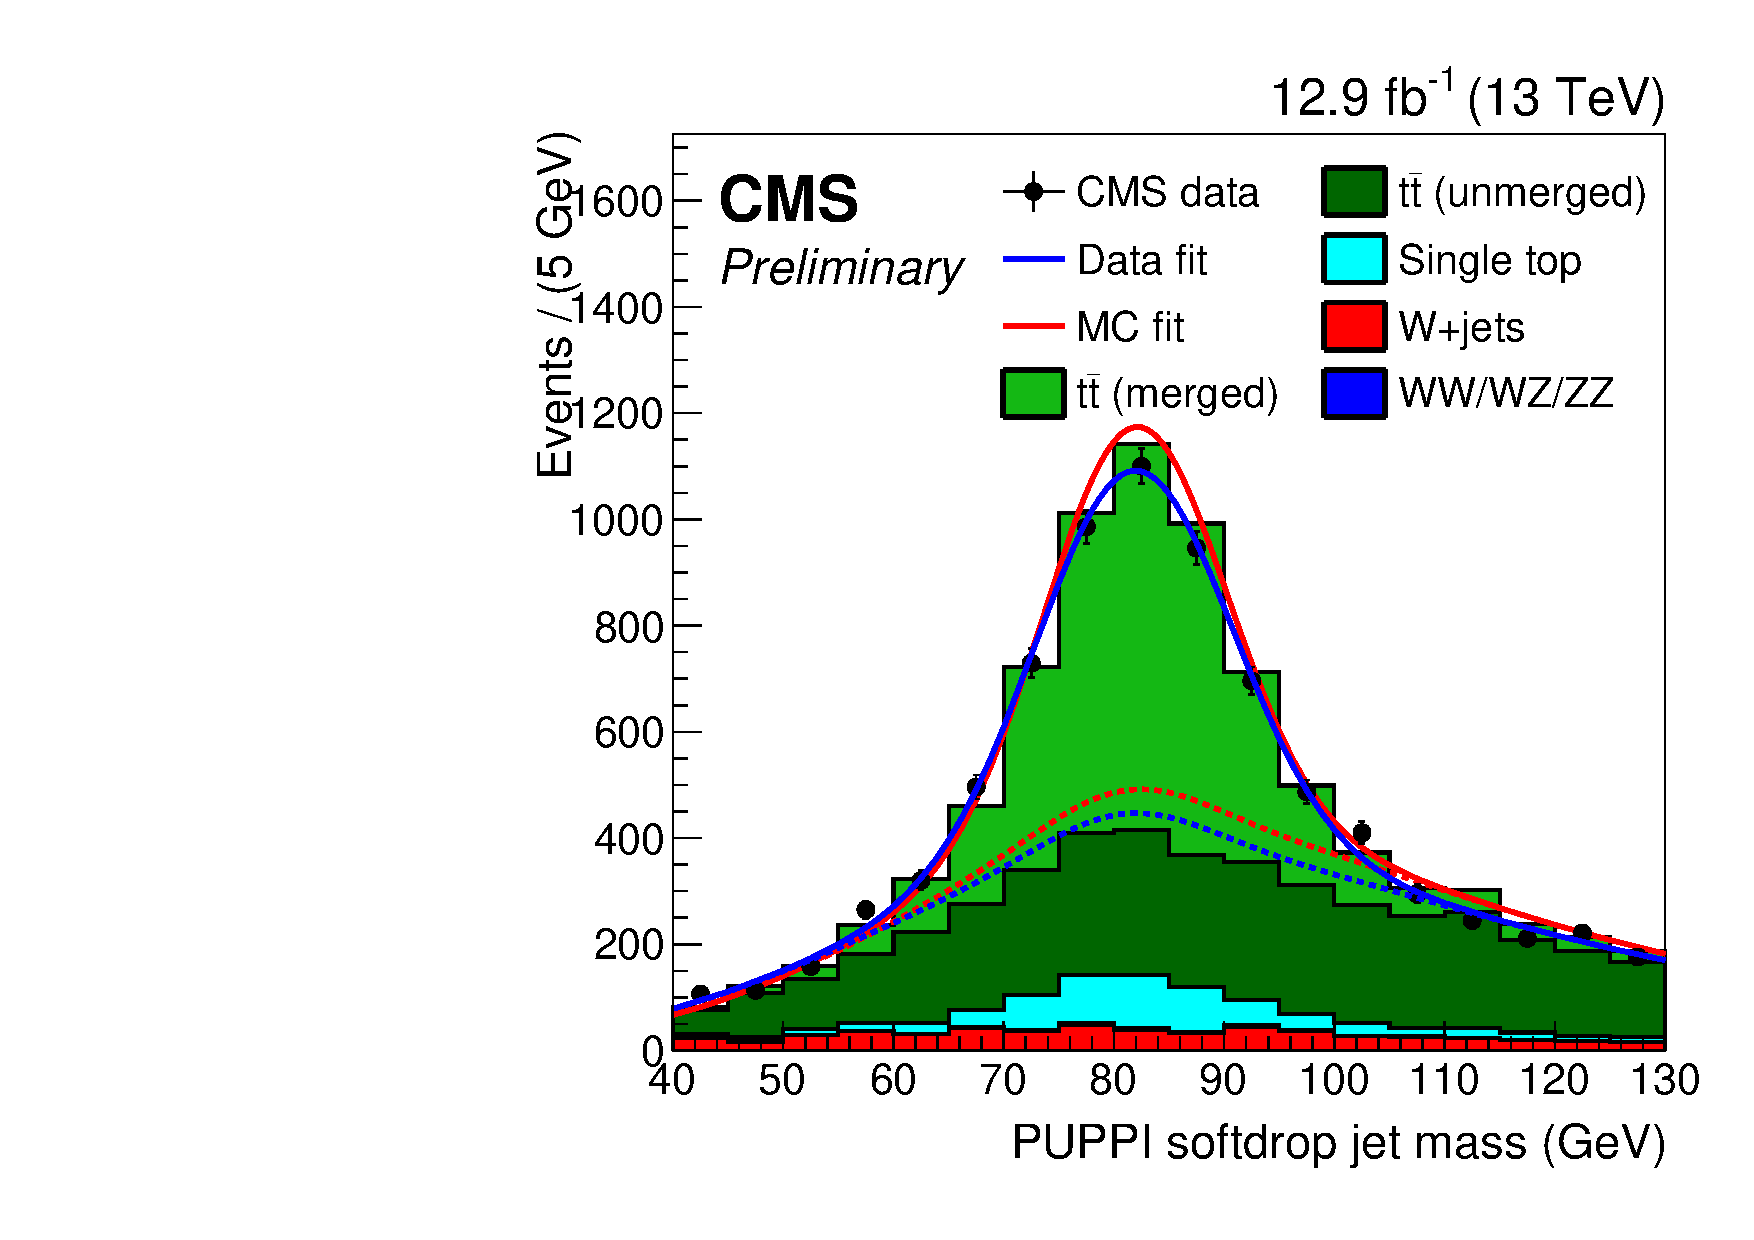
\includegraphics[width=0.44\textwidth]{figures/analysis/search2/AN-16-235/plots/TotalFit__HP0v40powheg_PuppiSD.pdf}      %12.9 fbinv
% 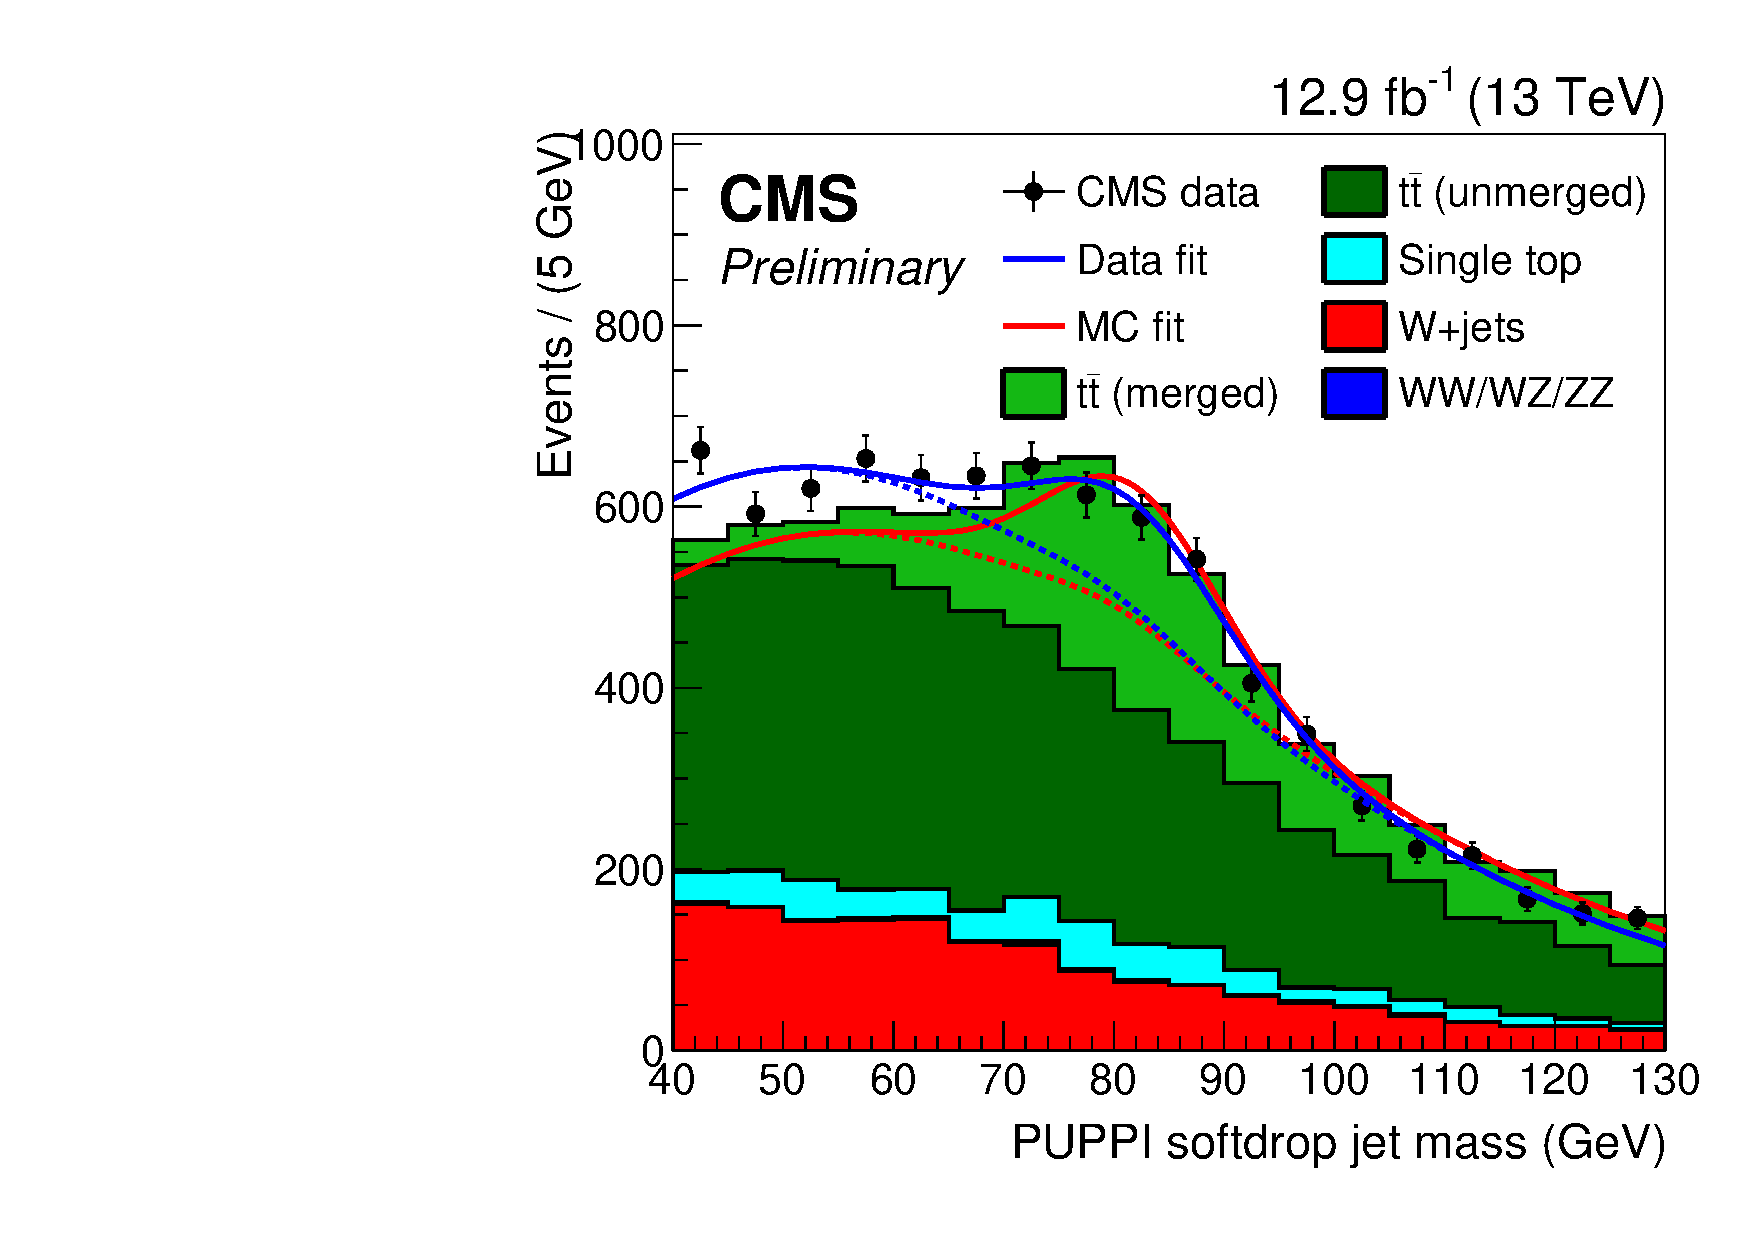
\includegraphics[width=0.44\textwidth]{figures/analysis/search2/AN-16-235/plots/TotalFit__HP0v40powheg_PuppiSD_fail.pdf} %12.9 fbinv
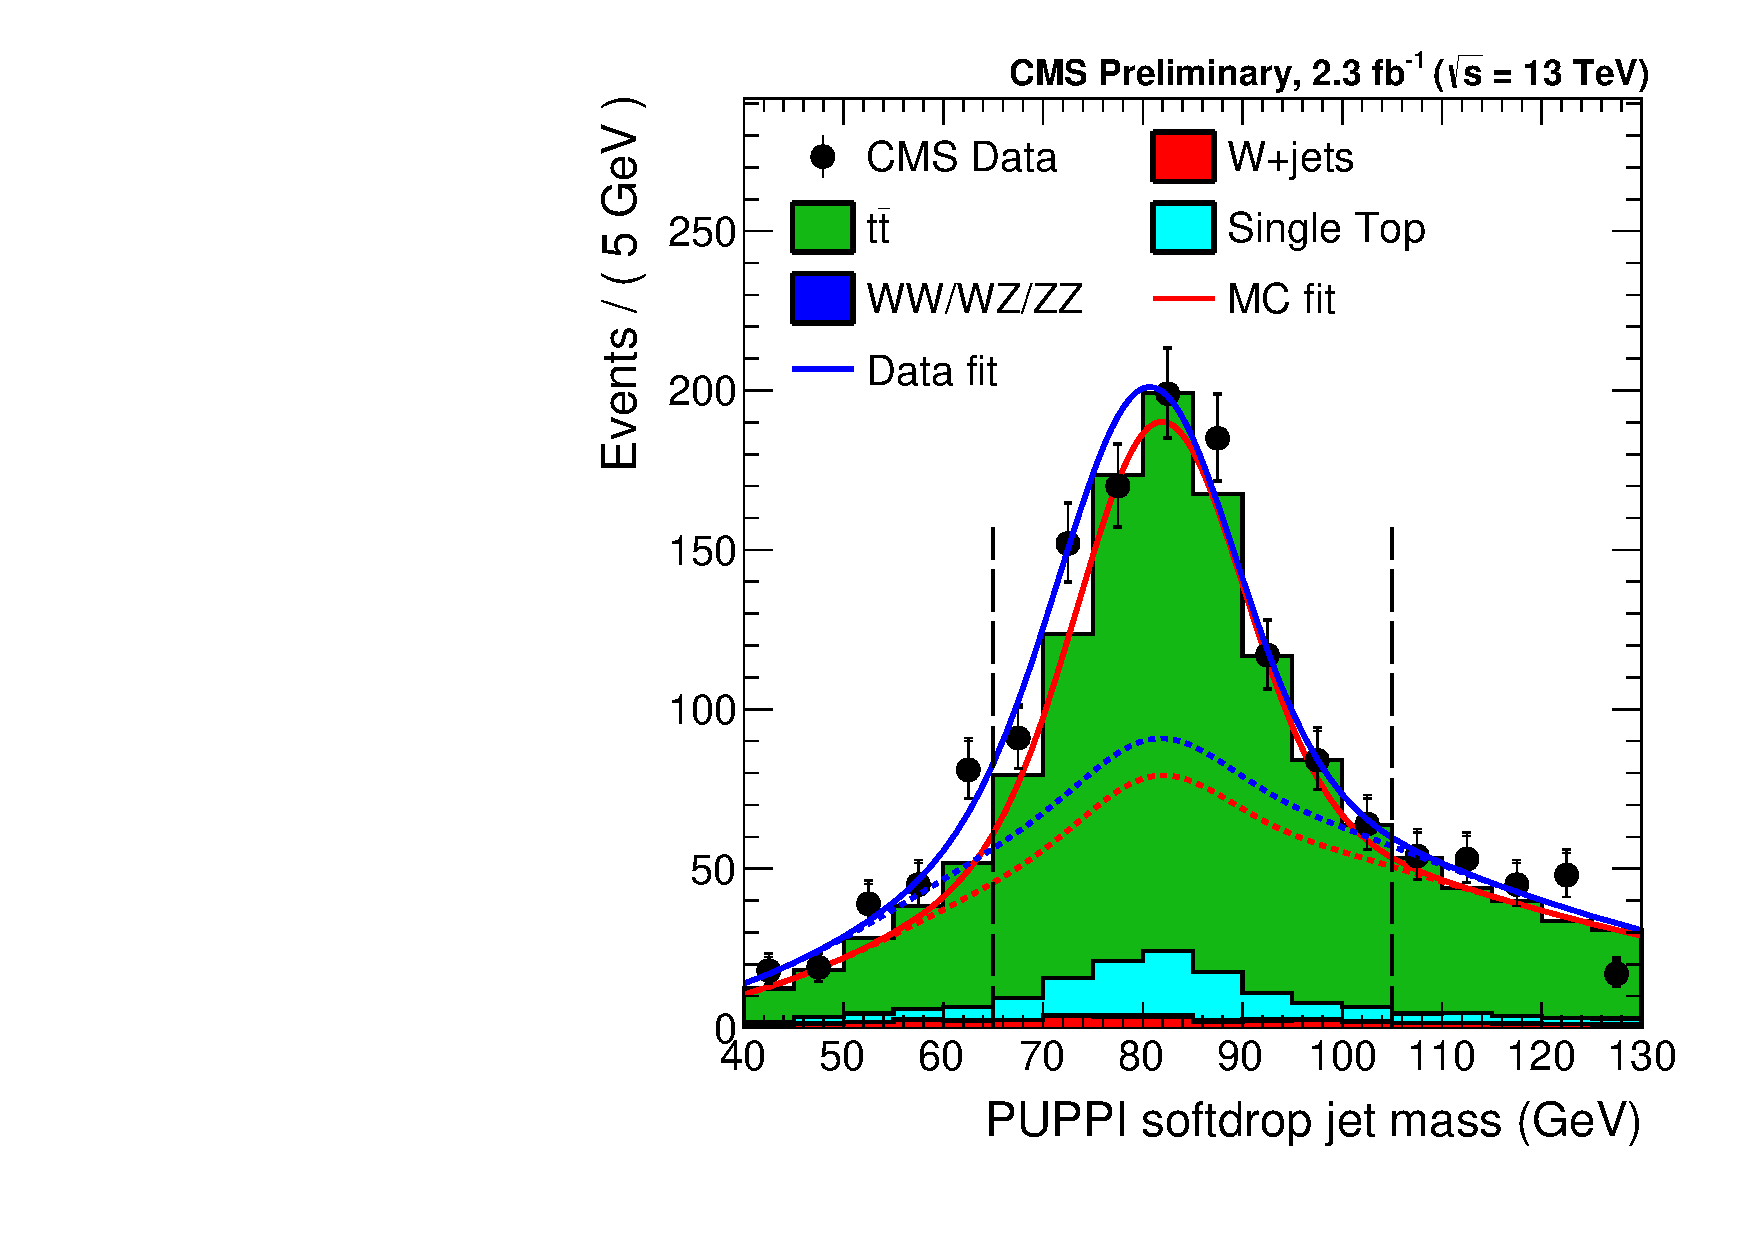
\includegraphics[width=0.44\textwidth]{figures/vtagging/AN-16-215/_HP0v40powheg_76X_PuppiSD_em_pTbin_200_5000.pdf}
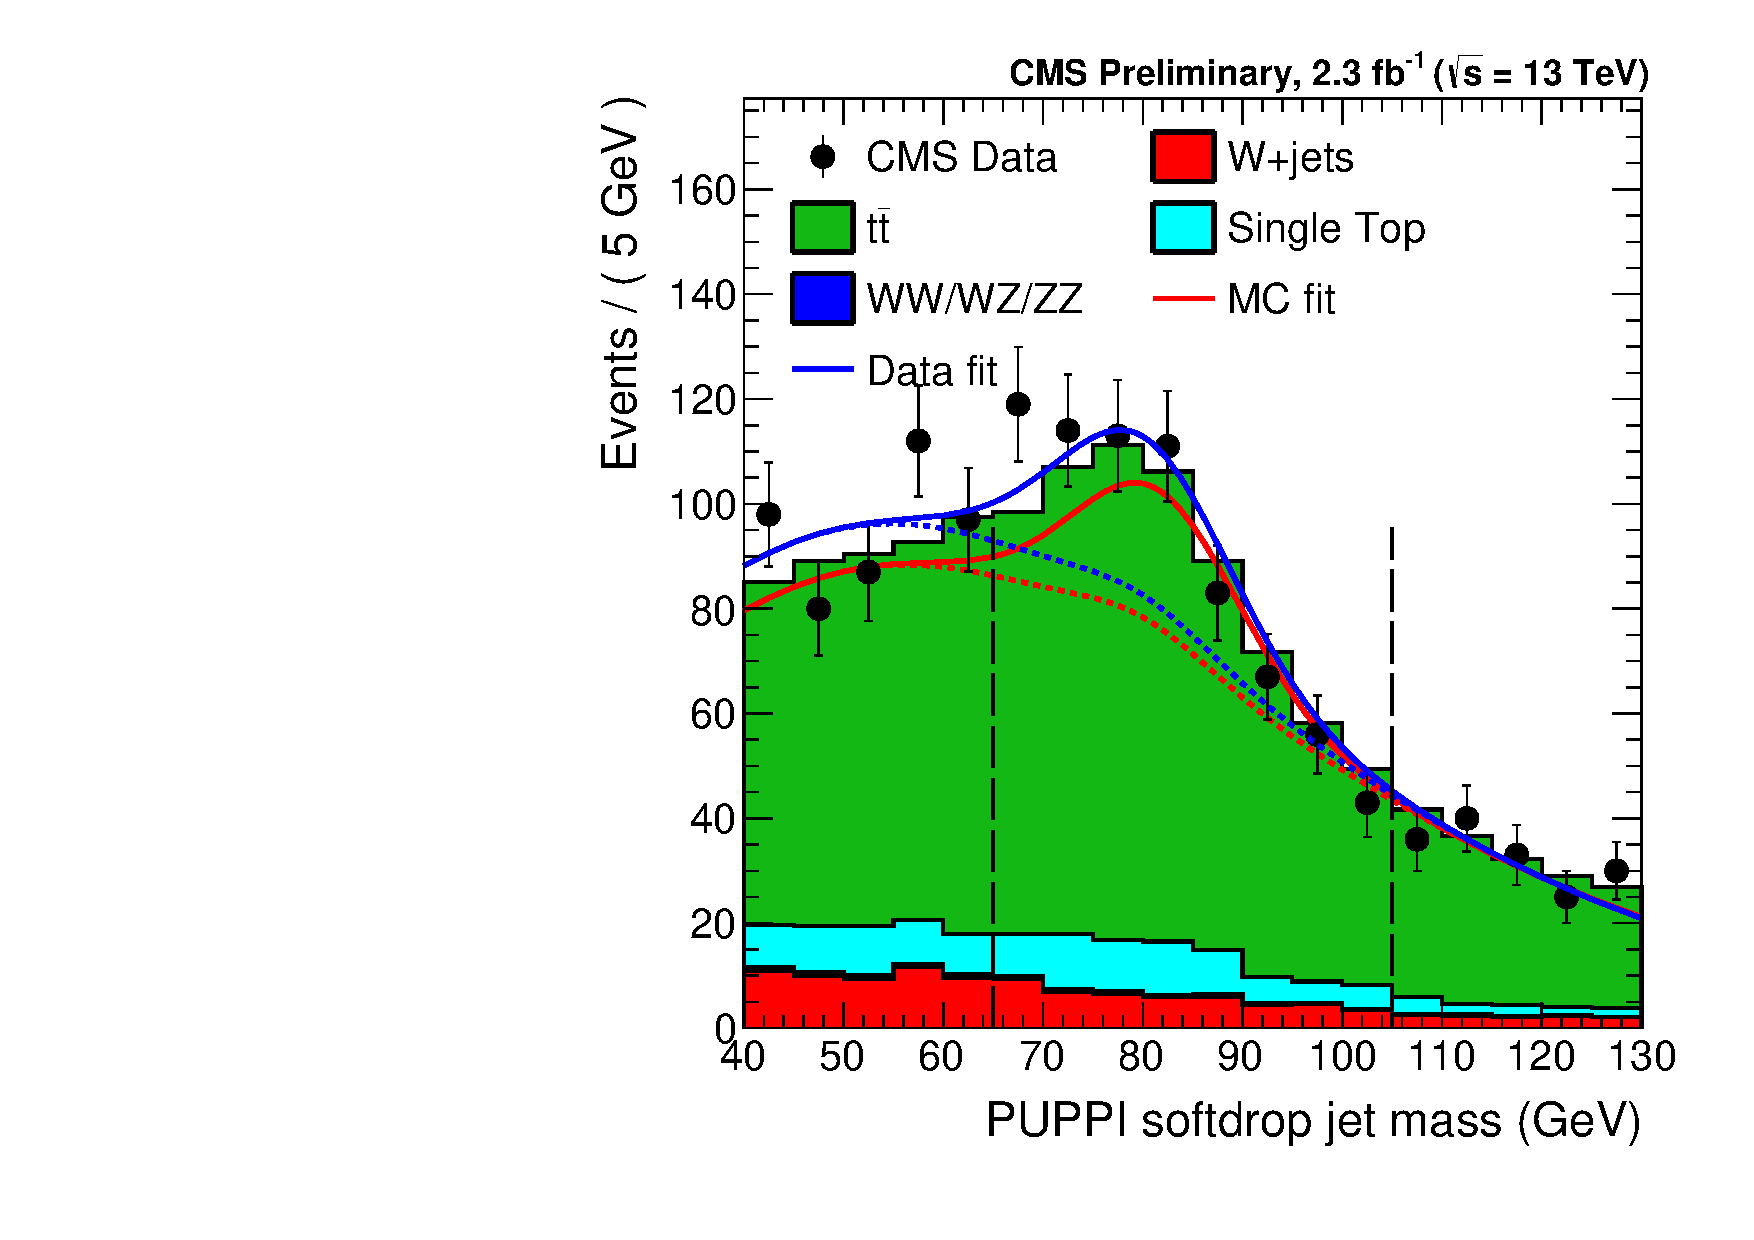
\includegraphics[width=0.44\textwidth]{figures/vtagging/AN-16-215/_HP0v40powheg_76X_PuppiSD_em_fail_pTbin_200_5000.pdf}\\
\caption{PUPPI softdrop jet mass distribution that pass (left) and fail (right) the PUPPI $\tau_2 / \tau_1 < 0.40$ selection. Results of both the fit to data (blue) and simulation (red) are shown and the background components of the fit are shown as short-dashed lines. (!RATHER REPLACE BY 12.9INVFB MEASUREMENT)}
\label{fig:searchII:simfit}
\end{figure}

Both scale factors are comparable to unity, within uncertainties. We additionally extract the jet mass scale and jet mass resolution from the mean and width, respectively, of the Gaussian
component of the total fit in the pass region. These are summarized in Table~\ref{tab:searchII:wtagparams}.  As for pruning (Table~\ref{tab:searchI:params}), we find that the W jet mass scale is larger in simulation than in data, of roughly 2\%.
The jet mass resolution, on the other hand, is larger in data, of roughly 7\%, whereas for pruning the resolution is larger in simulation (11\%). However, both are statistically insignificant and comparable with unity within uncertainties.

\begin{table}[!htb]
 \begin{center}

 \begin{tabular}{c|c|c|c}
  Parameter & Data & Simulation & Data/Simulation \\
  \hline
  PUPPI softdrop $\langle m \rangle$ & $80.3 \pm 0.8~{\rm \GeV}$ & $81.9 \pm 0.01~{\rm \GeV}$ & $0.98 \pm 0.01$ \\%New mass corrections
  PUPPI softdrop $\sigma$            & $ 9.0 \pm 0.9~{\rm \GeV}$ &  $8.5 \pm 0.4~{\rm \GeV}$  & $1.07 \pm 0.12$ \\%New mass corrections
  \hline
 \end{tabular}
 \caption{Summary of the fitted W-mass peak fit parameters.}
 \label{tab:searchII:wtagparams}
 \end{center}
\end{table}

The W-tagging efficiency scale factors, jet mass scale and resolution affects the signal yield and are included as described in Section~\ref{sec:searchI:wtagimpact}: as a scale of the total signal yield and an uncertainty on the signal efficiency due to
a shift and broadening of the \PW-jet mass peak.
%  % \begin{figure}[htbp]
% %  \centering
% %  \begin{tabular}{cc}
% %  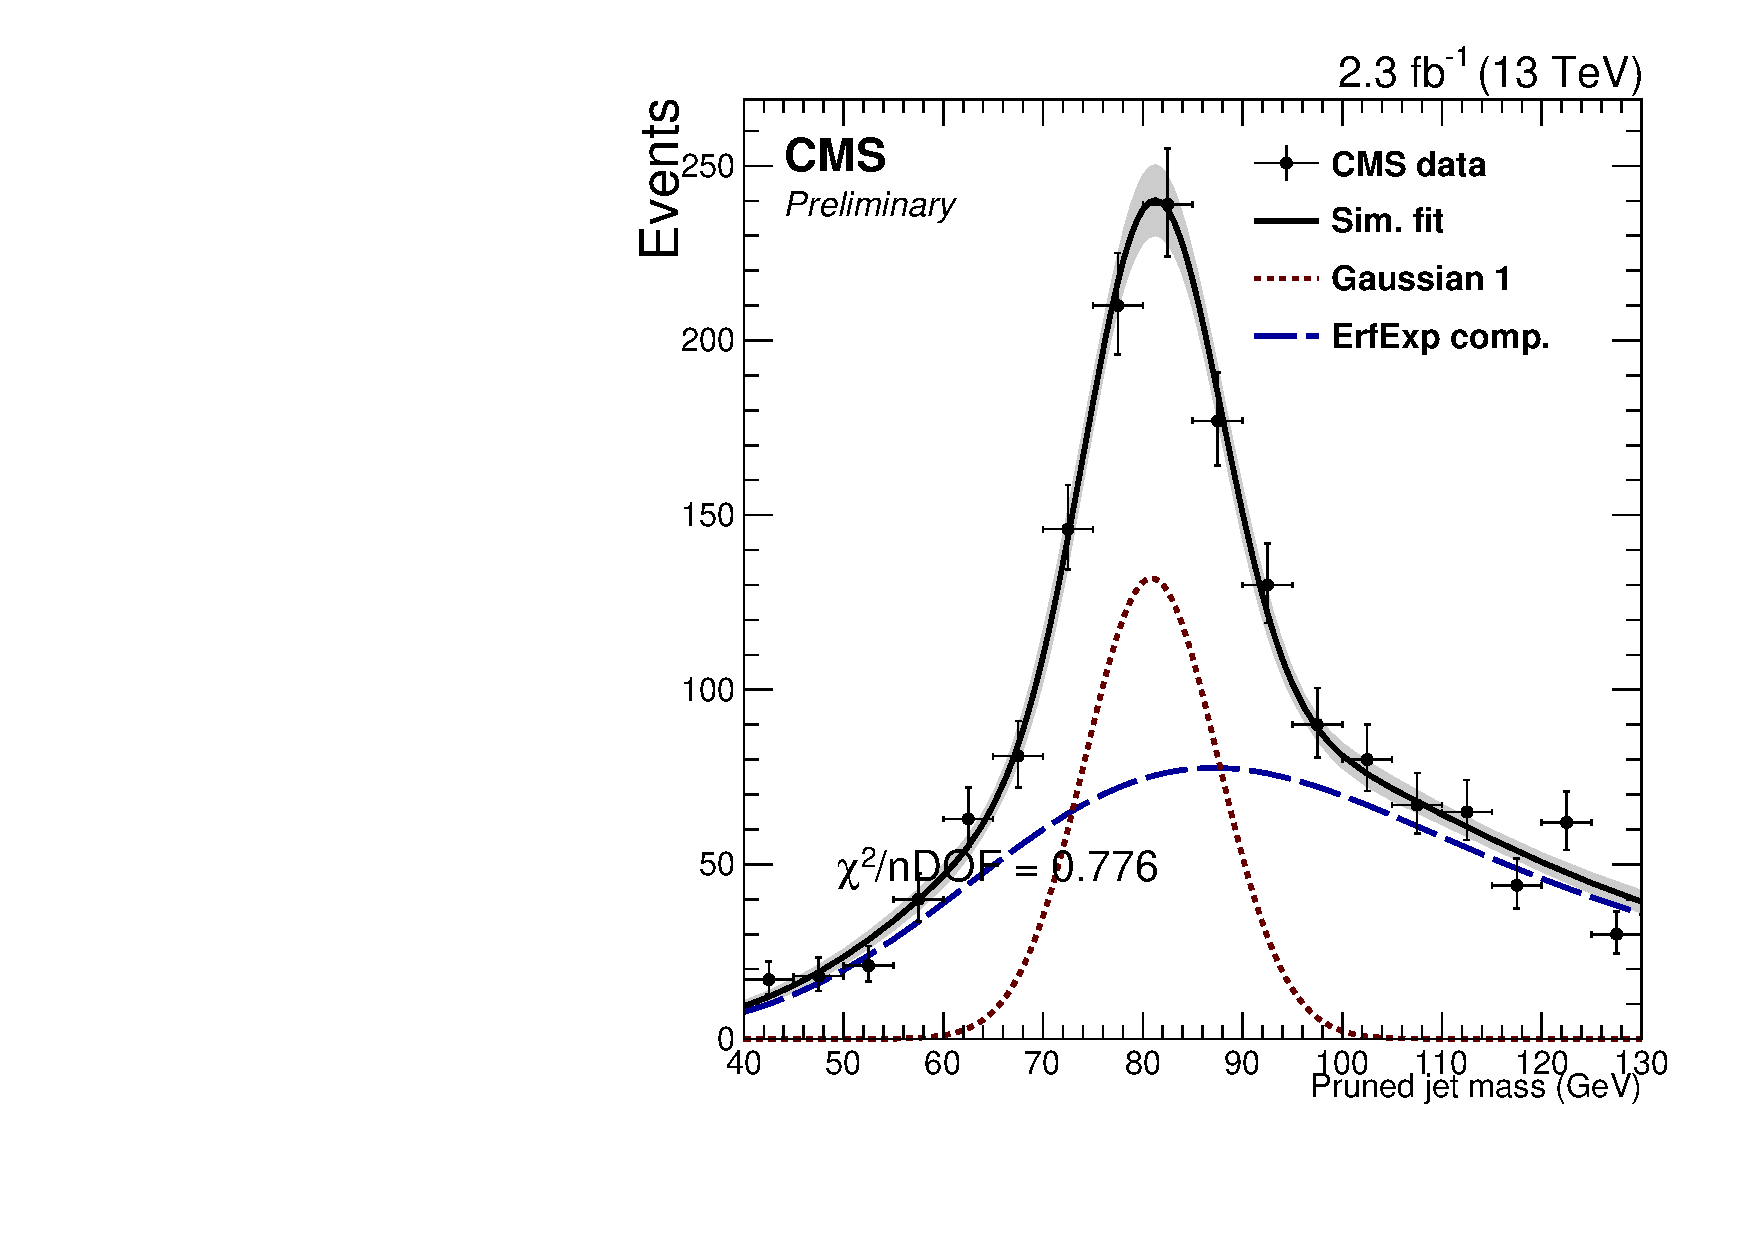
\includegraphics[width=0.45\textwidth]{figures/vtagging/AN-16-215/plots_76X/plots_0v45/model_data_em.pdf}
% %  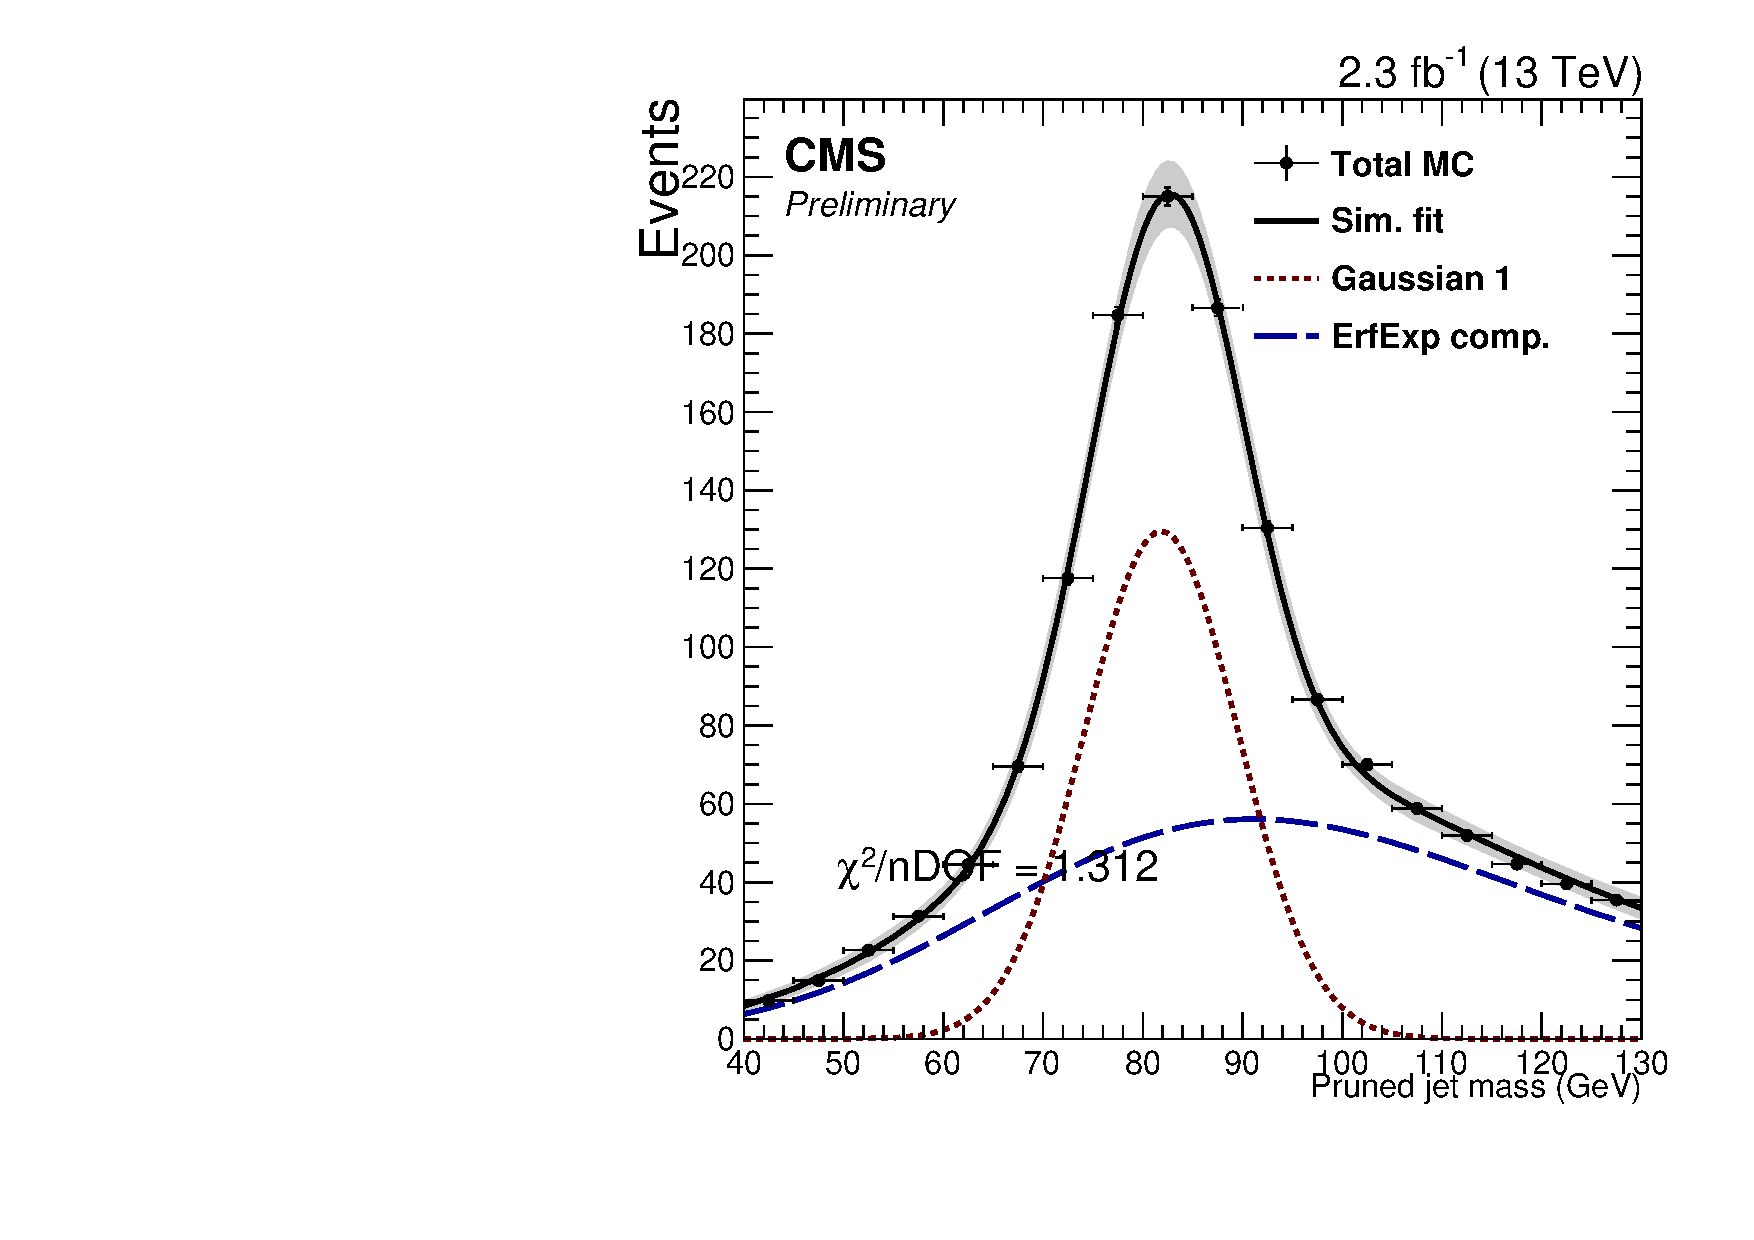
\includegraphics[width=0.45\textwidth]{figures/vtagging/AN-16-215/plots_76X/plots_0v45/model_TotalMC_em.pdf}\\
% %  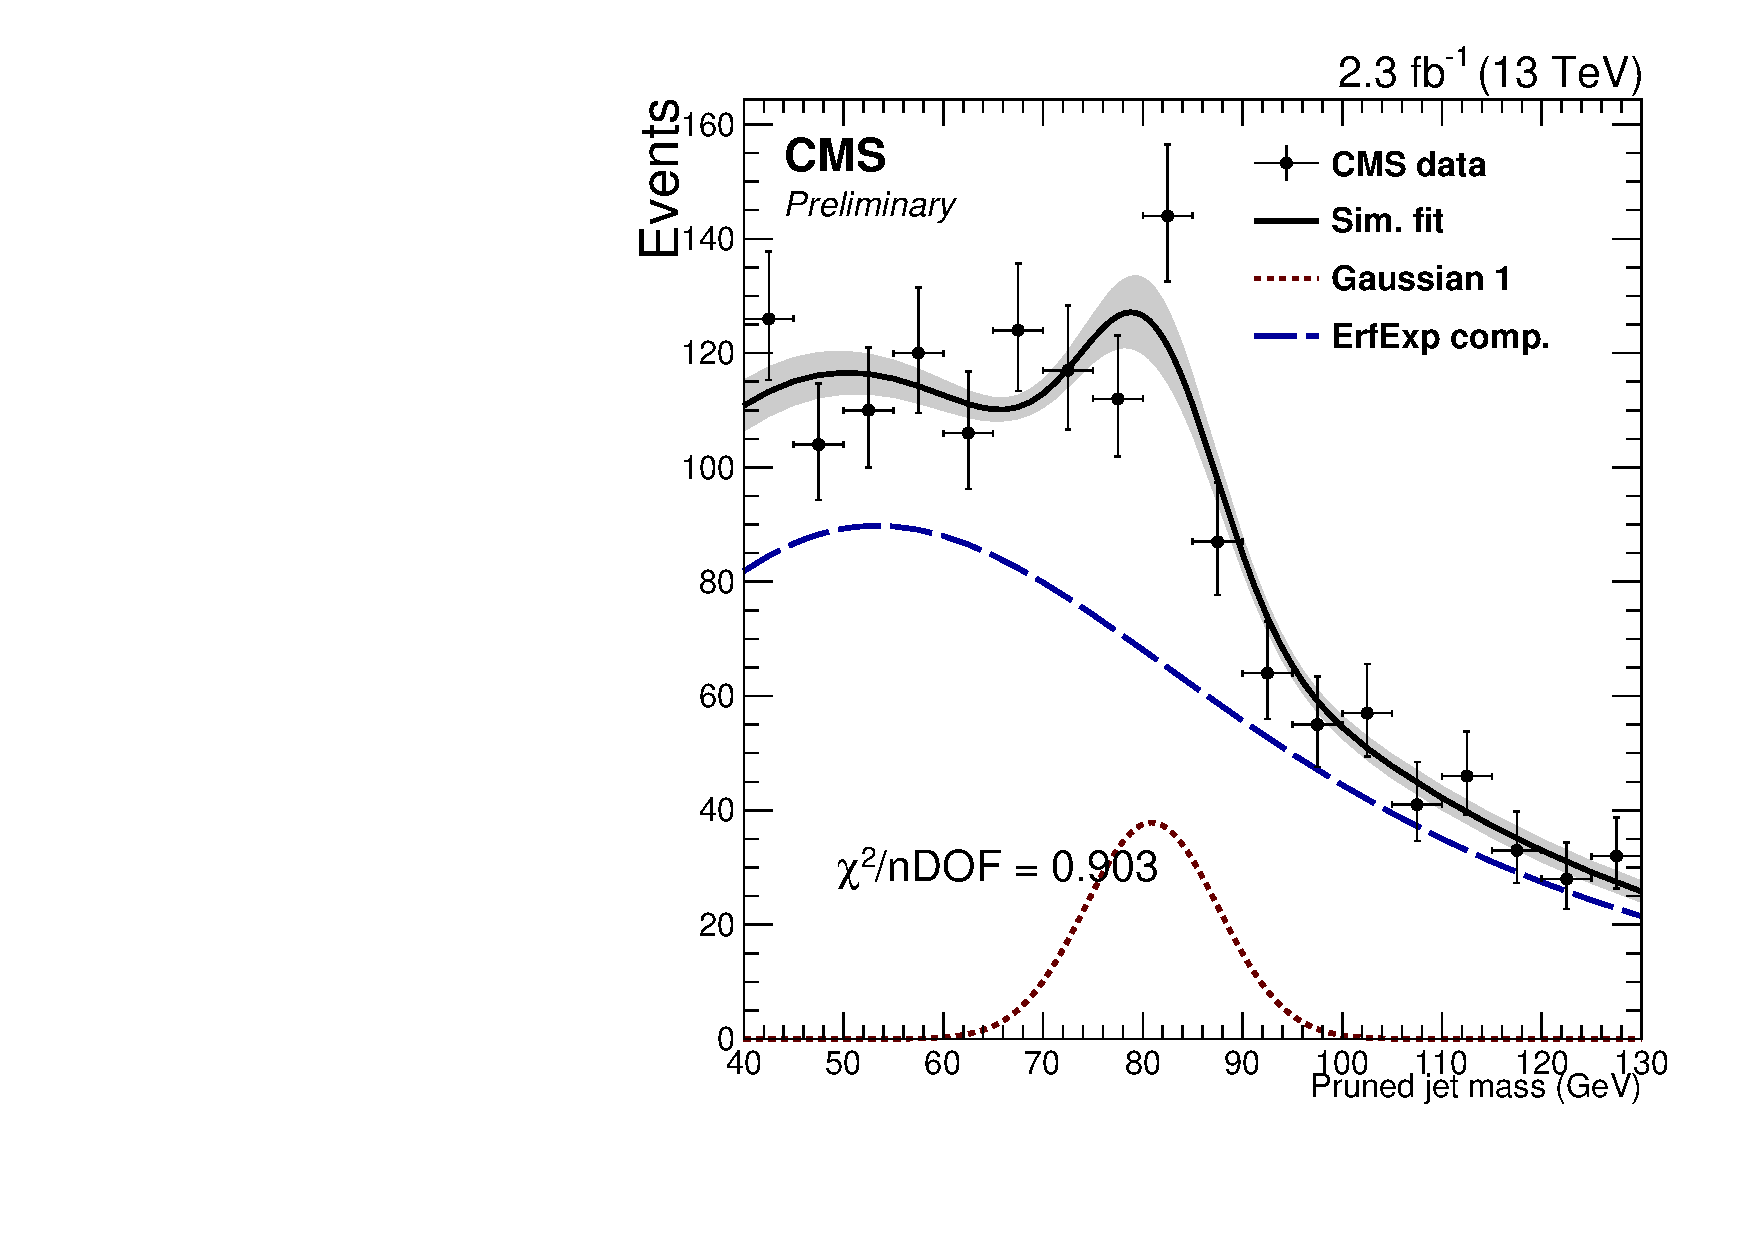
\includegraphics[width=0.45\textwidth]{figures/vtagging/AN-16-215/plots_76X/plots_0v45/model_data_failtau2tau1cut_em.pdf}
% %  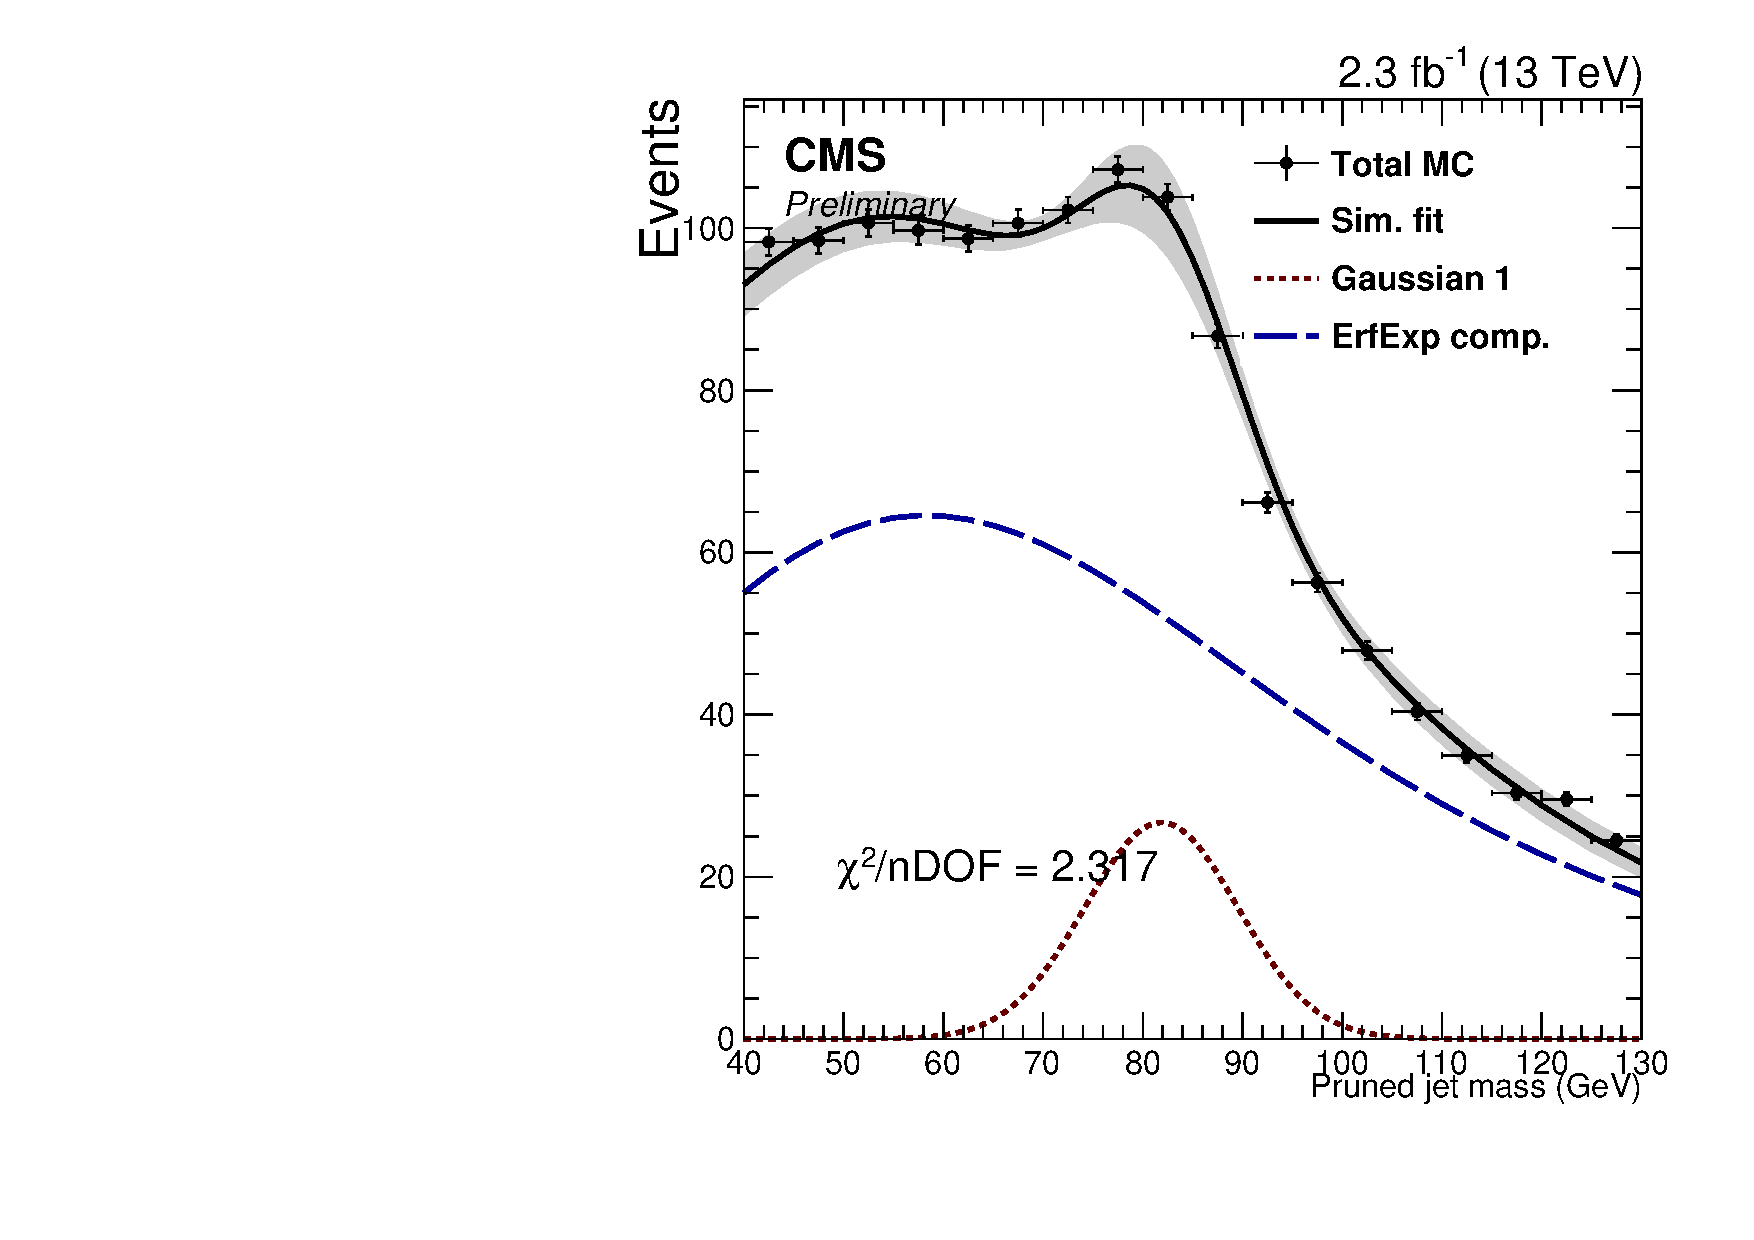
\includegraphics[width=0.45\textwidth]{figures/vtagging/AN-16-215/plots_76X/plots_0v45/model_TotalMC_failtau2tau1cut_em.pdf}\\
% %  \end{tabular}
% %  \caption{Fit results in data (left) and simulation (right) after simultaneous fit.
% % Top: pass selection($\tau_{21} < 0.45$), bottom: fail selection($\tau_{21} > 0.45$). }
% %  \label{fig:Wtagging_sf_045}
% %  \end{figure}
% %
% %   \begin{figure}[htbp]
% %   \centering
% %   \begin{tabular}{cc}
% %   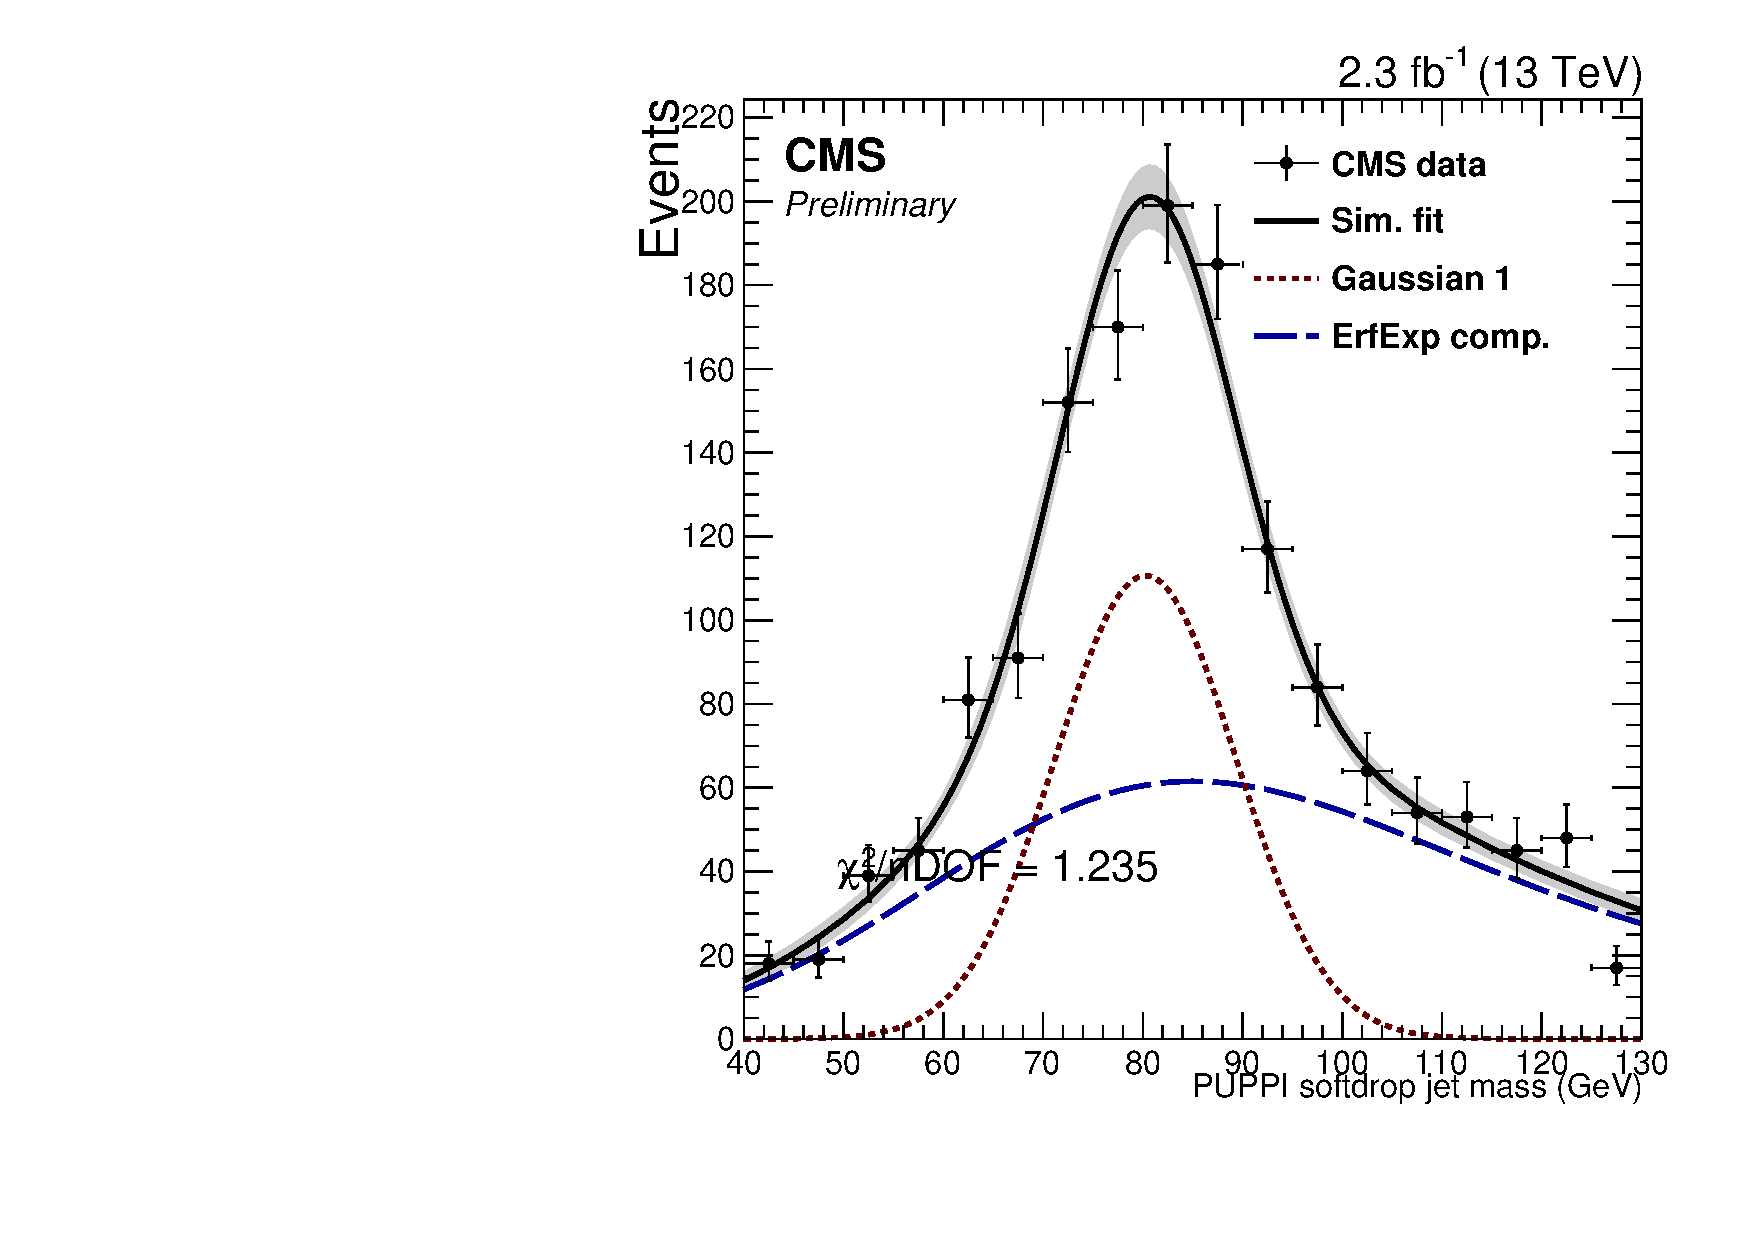
\includegraphics[width=0.45\textwidth]{figures/vtagging/AN-16-215/model_data_em.pdf}
% %   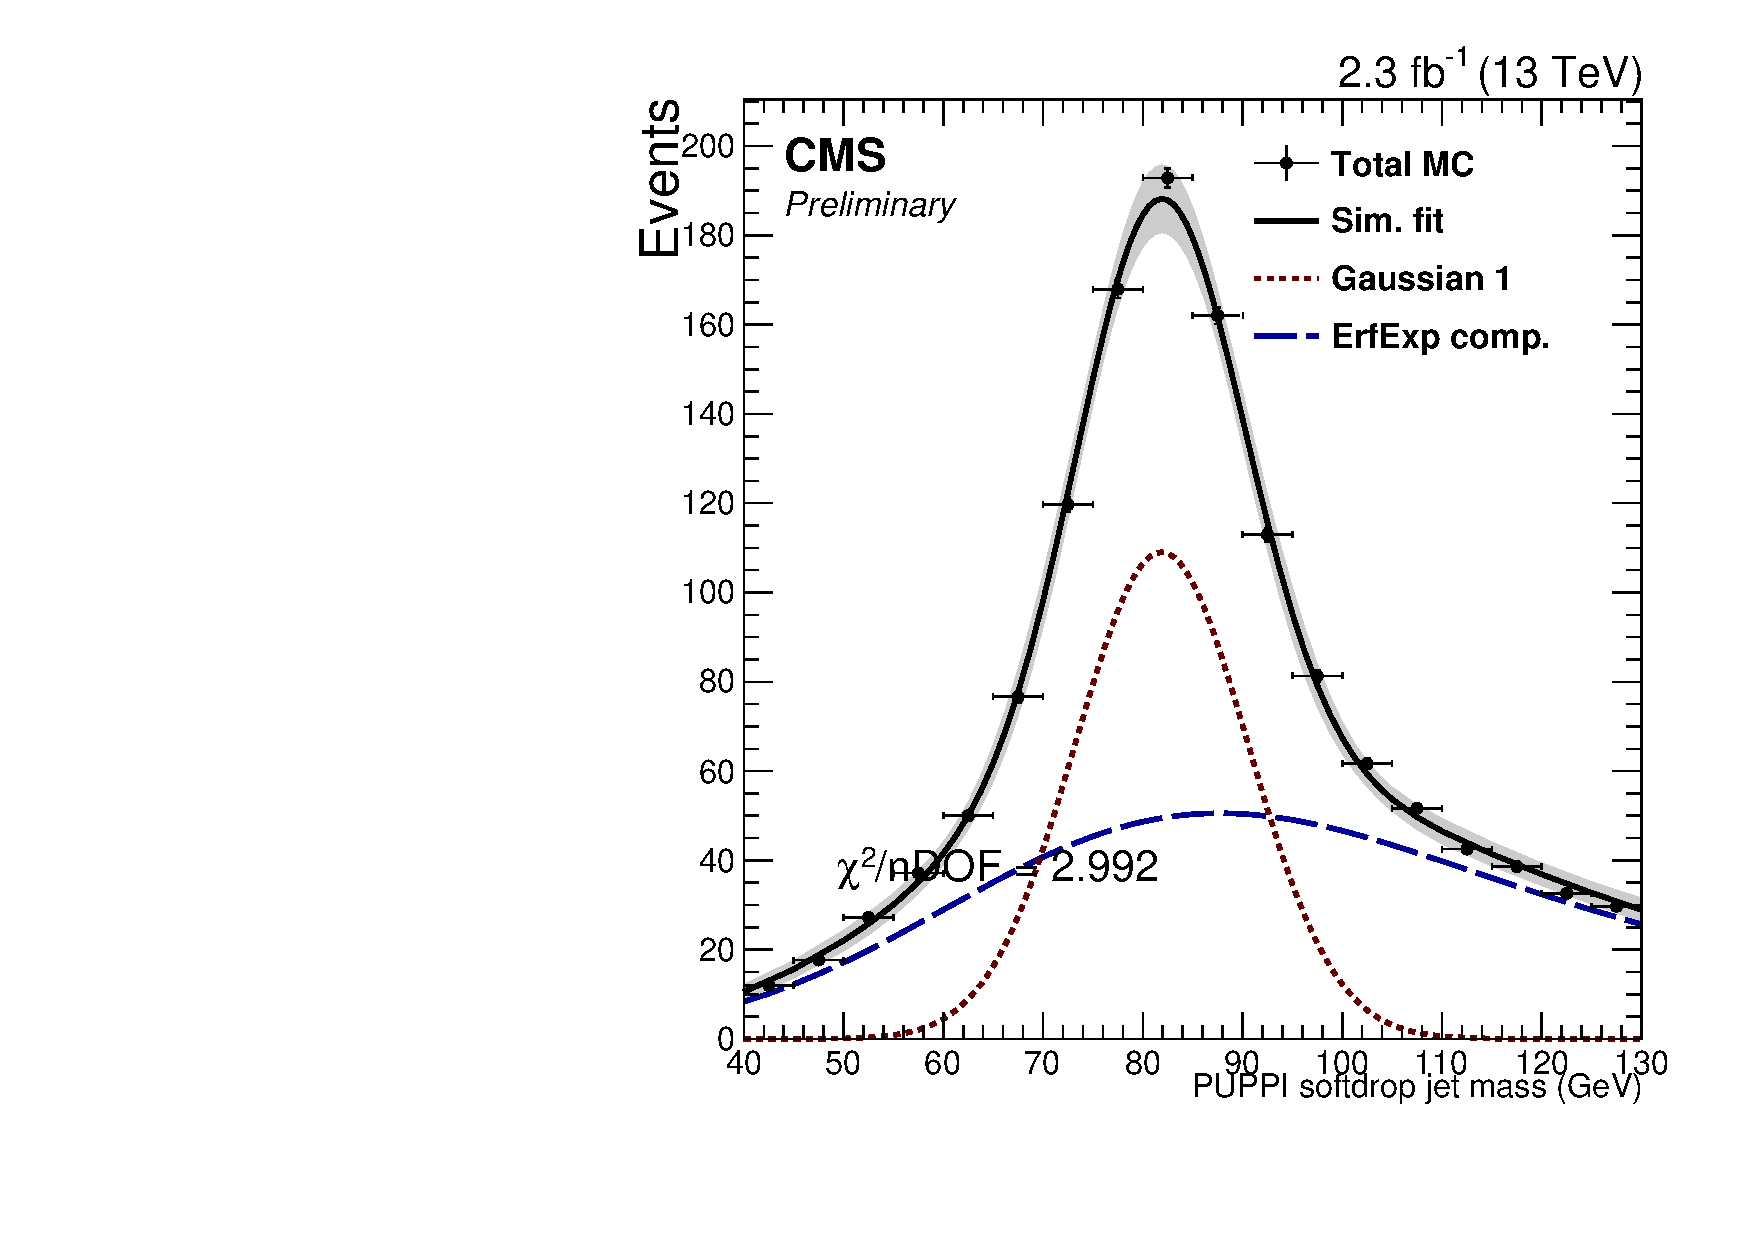
\includegraphics[width=0.45\textwidth]{figures/vtagging/AN-16-215/model_TotalMC_em.pdf}\\
% %   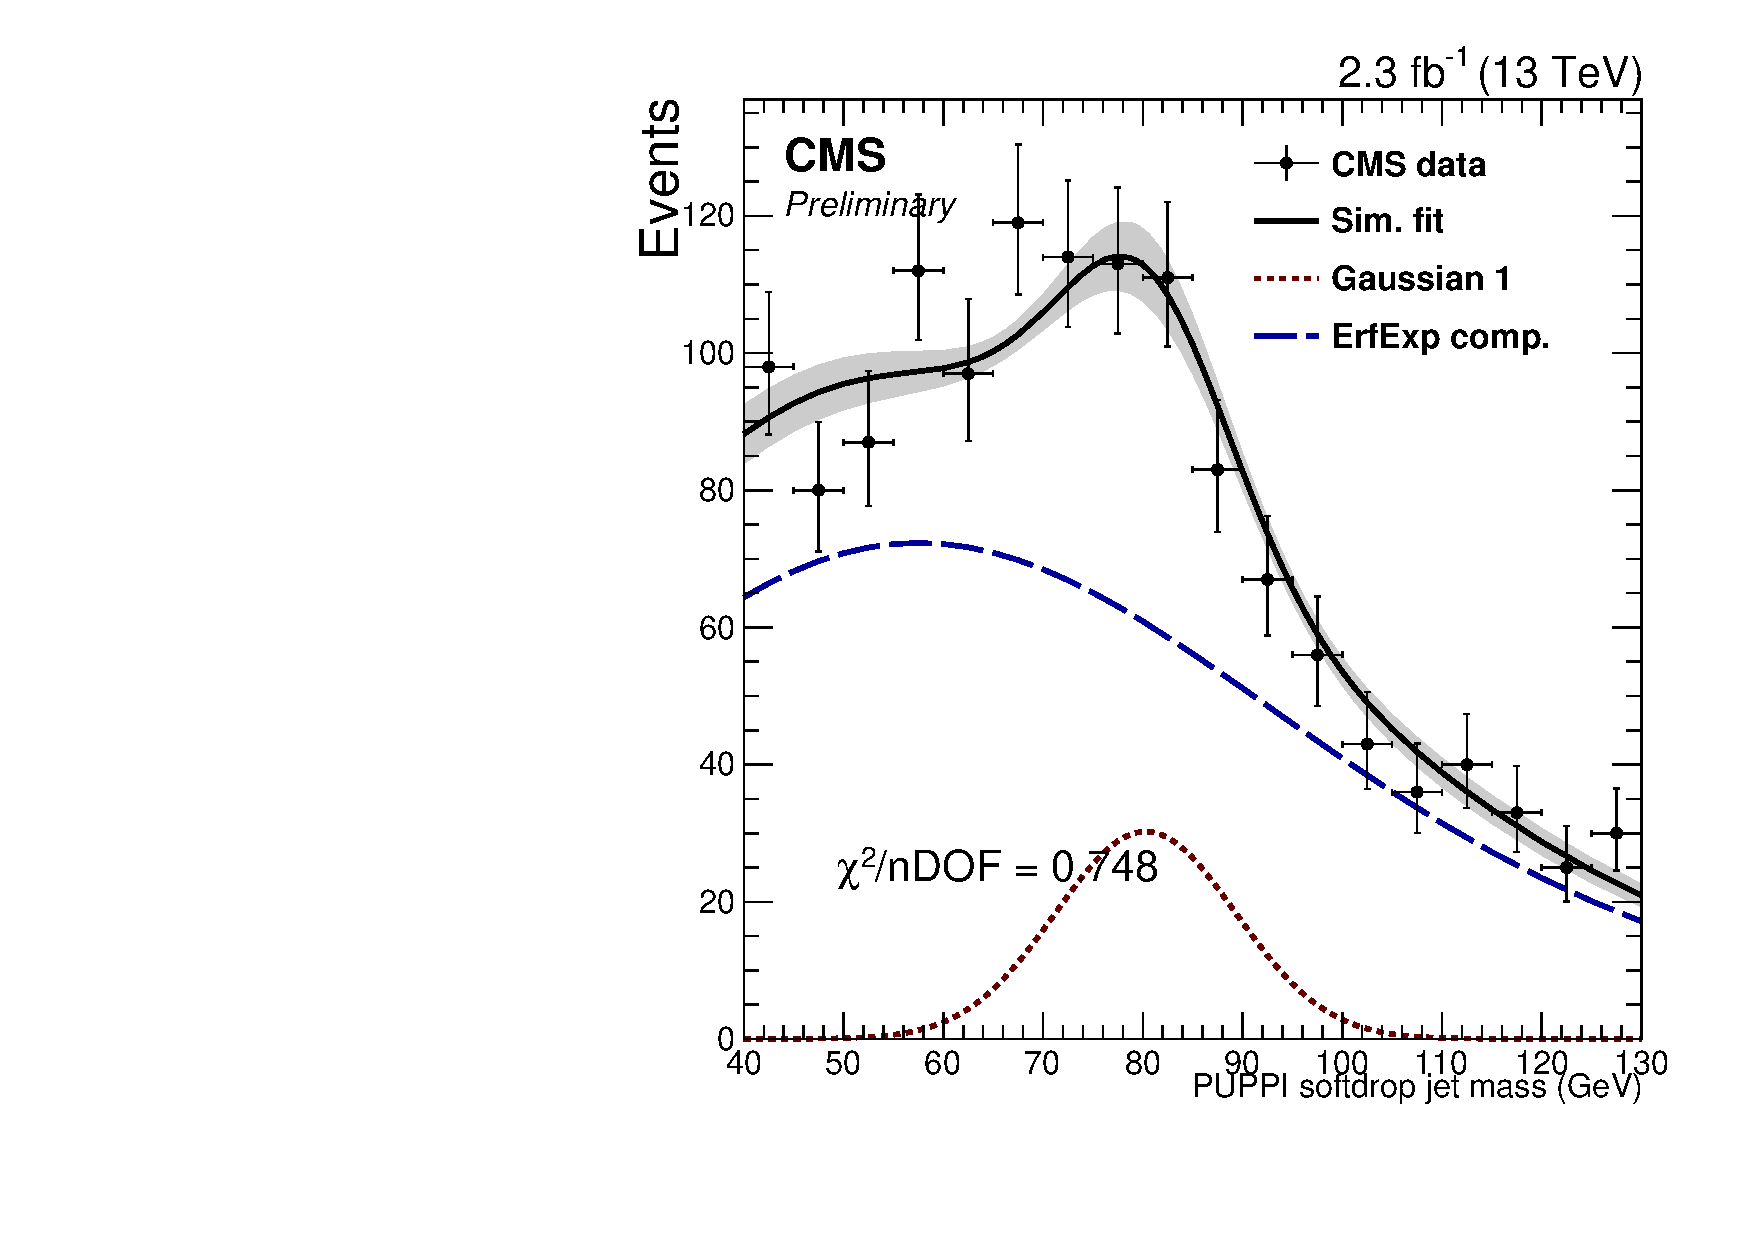
\includegraphics[width=0.45\textwidth]{figures/vtagging/AN-16-215/model_data_failtau2tau1cut_em.pdf}
% %   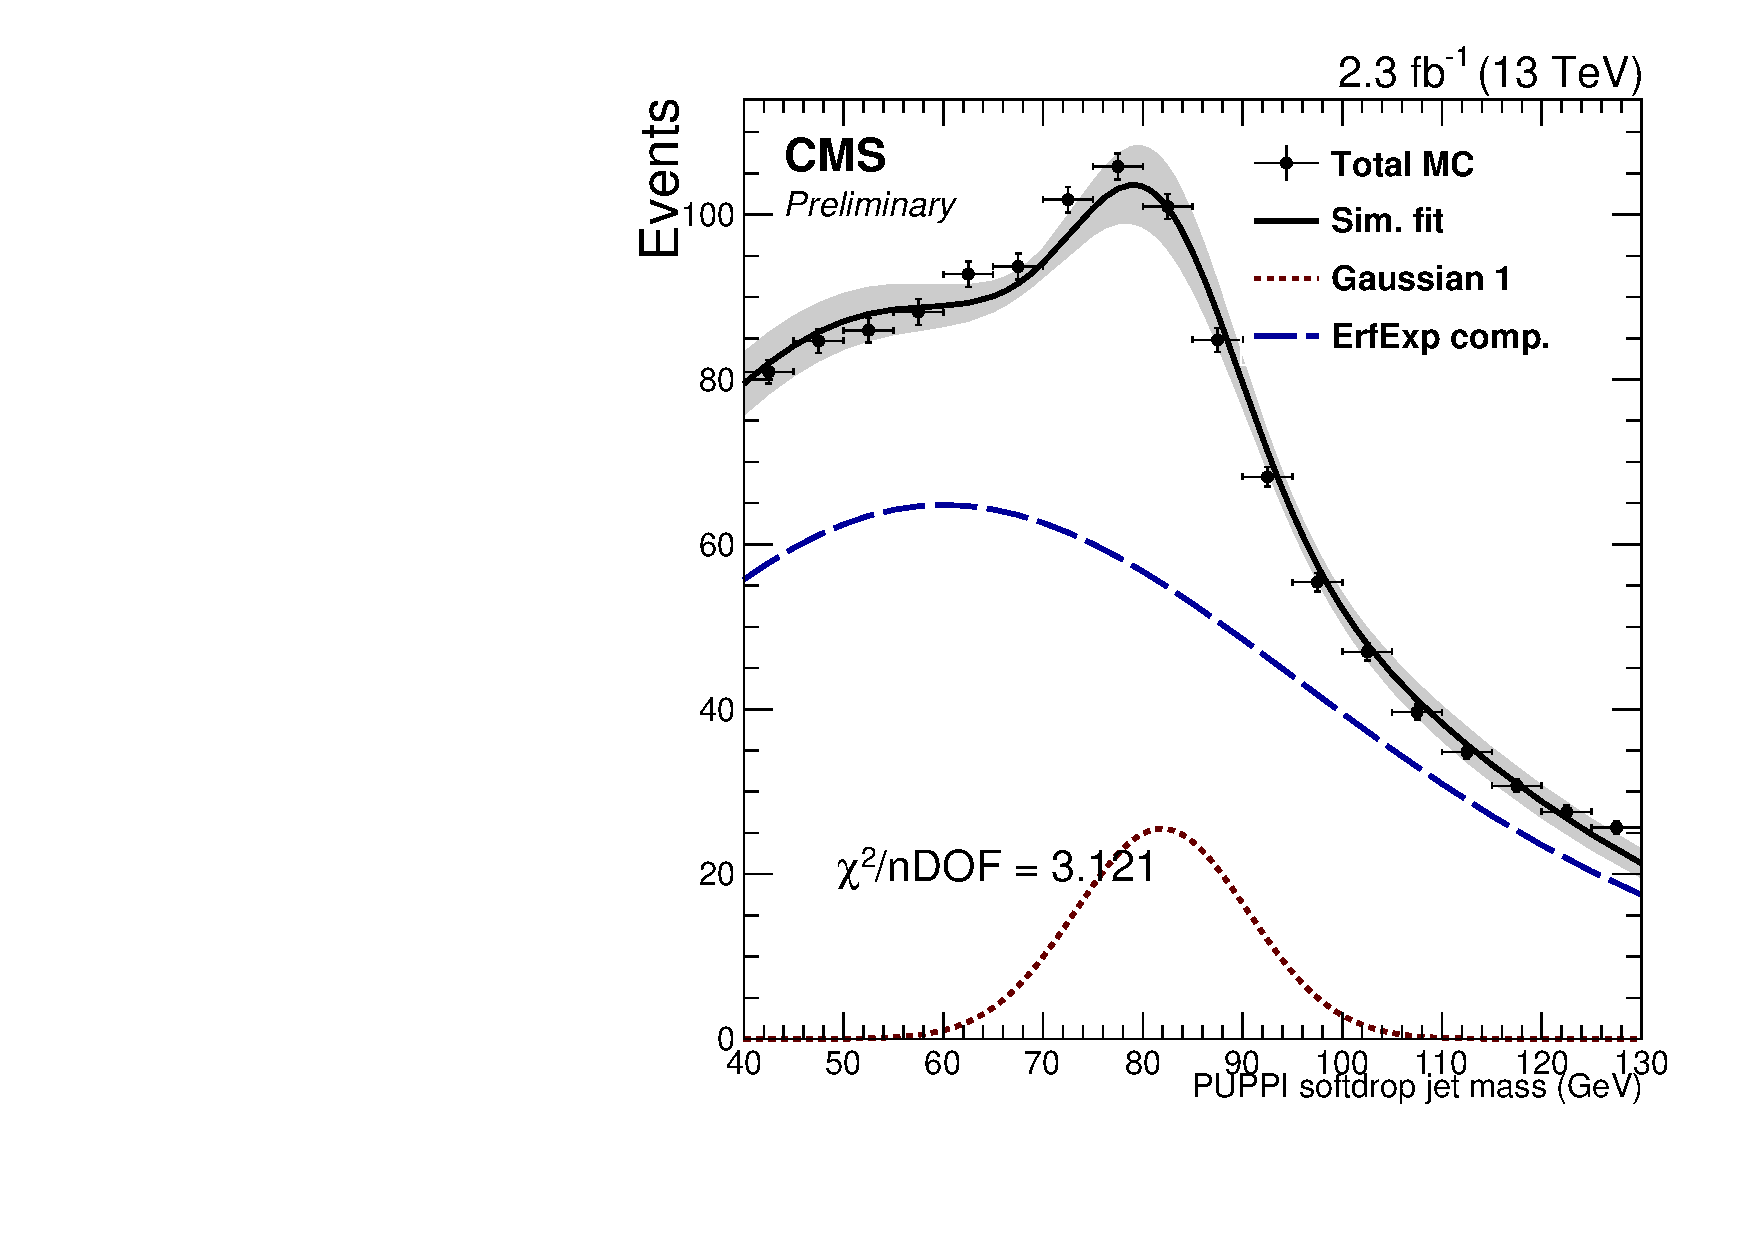
\includegraphics[width=0.45\textwidth]{figures/vtagging/AN-16-215/model_TotalMC_failtau2tau1cut_em.pdf}\\
% %   \end{tabular}
% %   \caption{Fit results in data (left) and simulation (right) after simultaneous fit.
% %  Top: pass selection(PUPPI $\tau_{21} < 0.40$), bottom: fail selection(PUPPI $\tau_{21} > 0.40$). }
% %   \label{fig:Wtagging_sf_040}
% %   \end{figure}
%

\subsection{W-tagging mistagging rate measurement} 
\label{sec:searchII:wmistag}
We additionally measure the W-tagging fake rate in data in a QCD dijet enriched region and compare this to the prediction from QCD MC using the three different combination of generators: \HERWIG{++}, \PYTHIA and \MADGRAPH+\PYTHIA.
Figure~\ref{fig:searchII:fakerate} shows the mistag rate as a function of \PT for three different taggers: CHS pruning + \nsubj, PUPPI softdrop + PUPPI \nsubj and PUPPI softdrop + \ddt.
\begin{figure}[htbp]
\centering
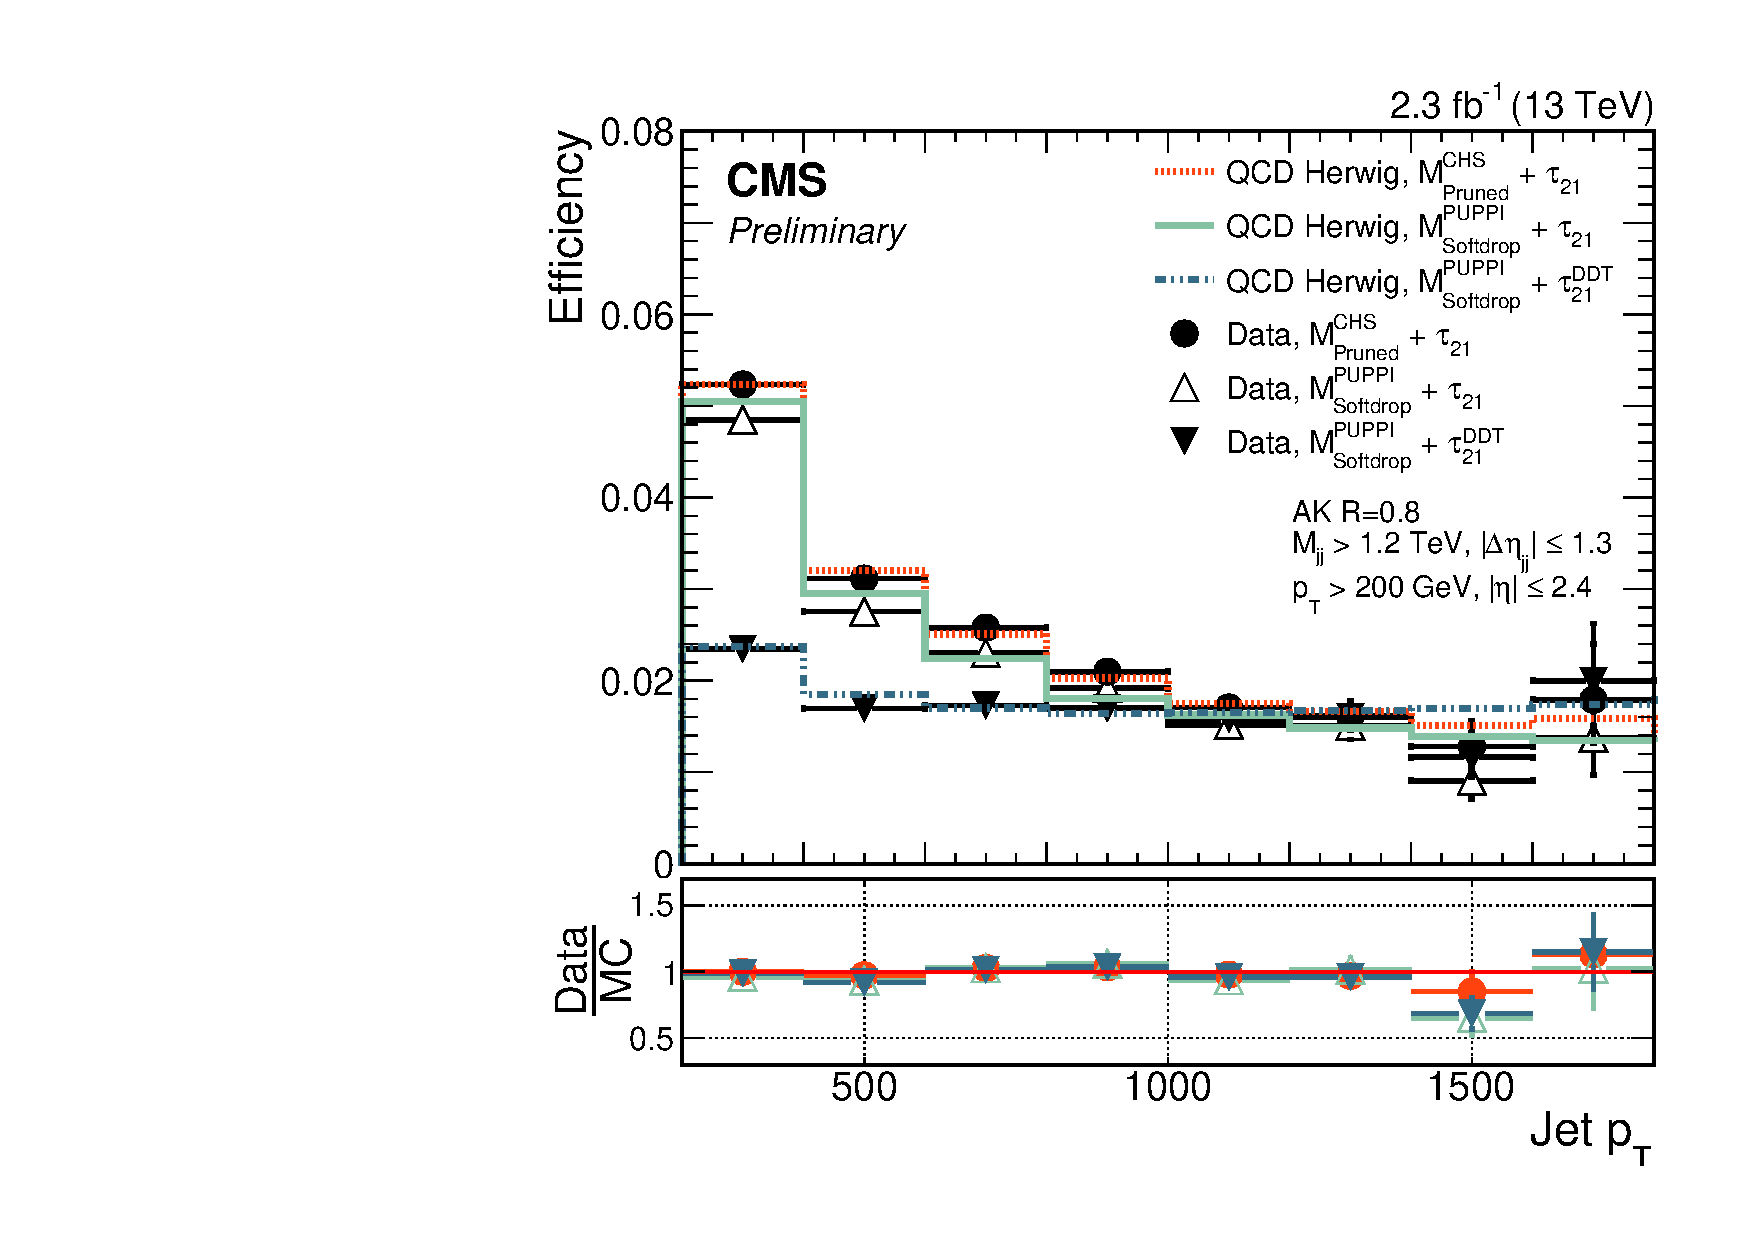
\includegraphics[width=0.49\textwidth]{figures/vtagging/JME-16-003/BoostedW/BkgEff_DataMC_herwig_pT.pdf}
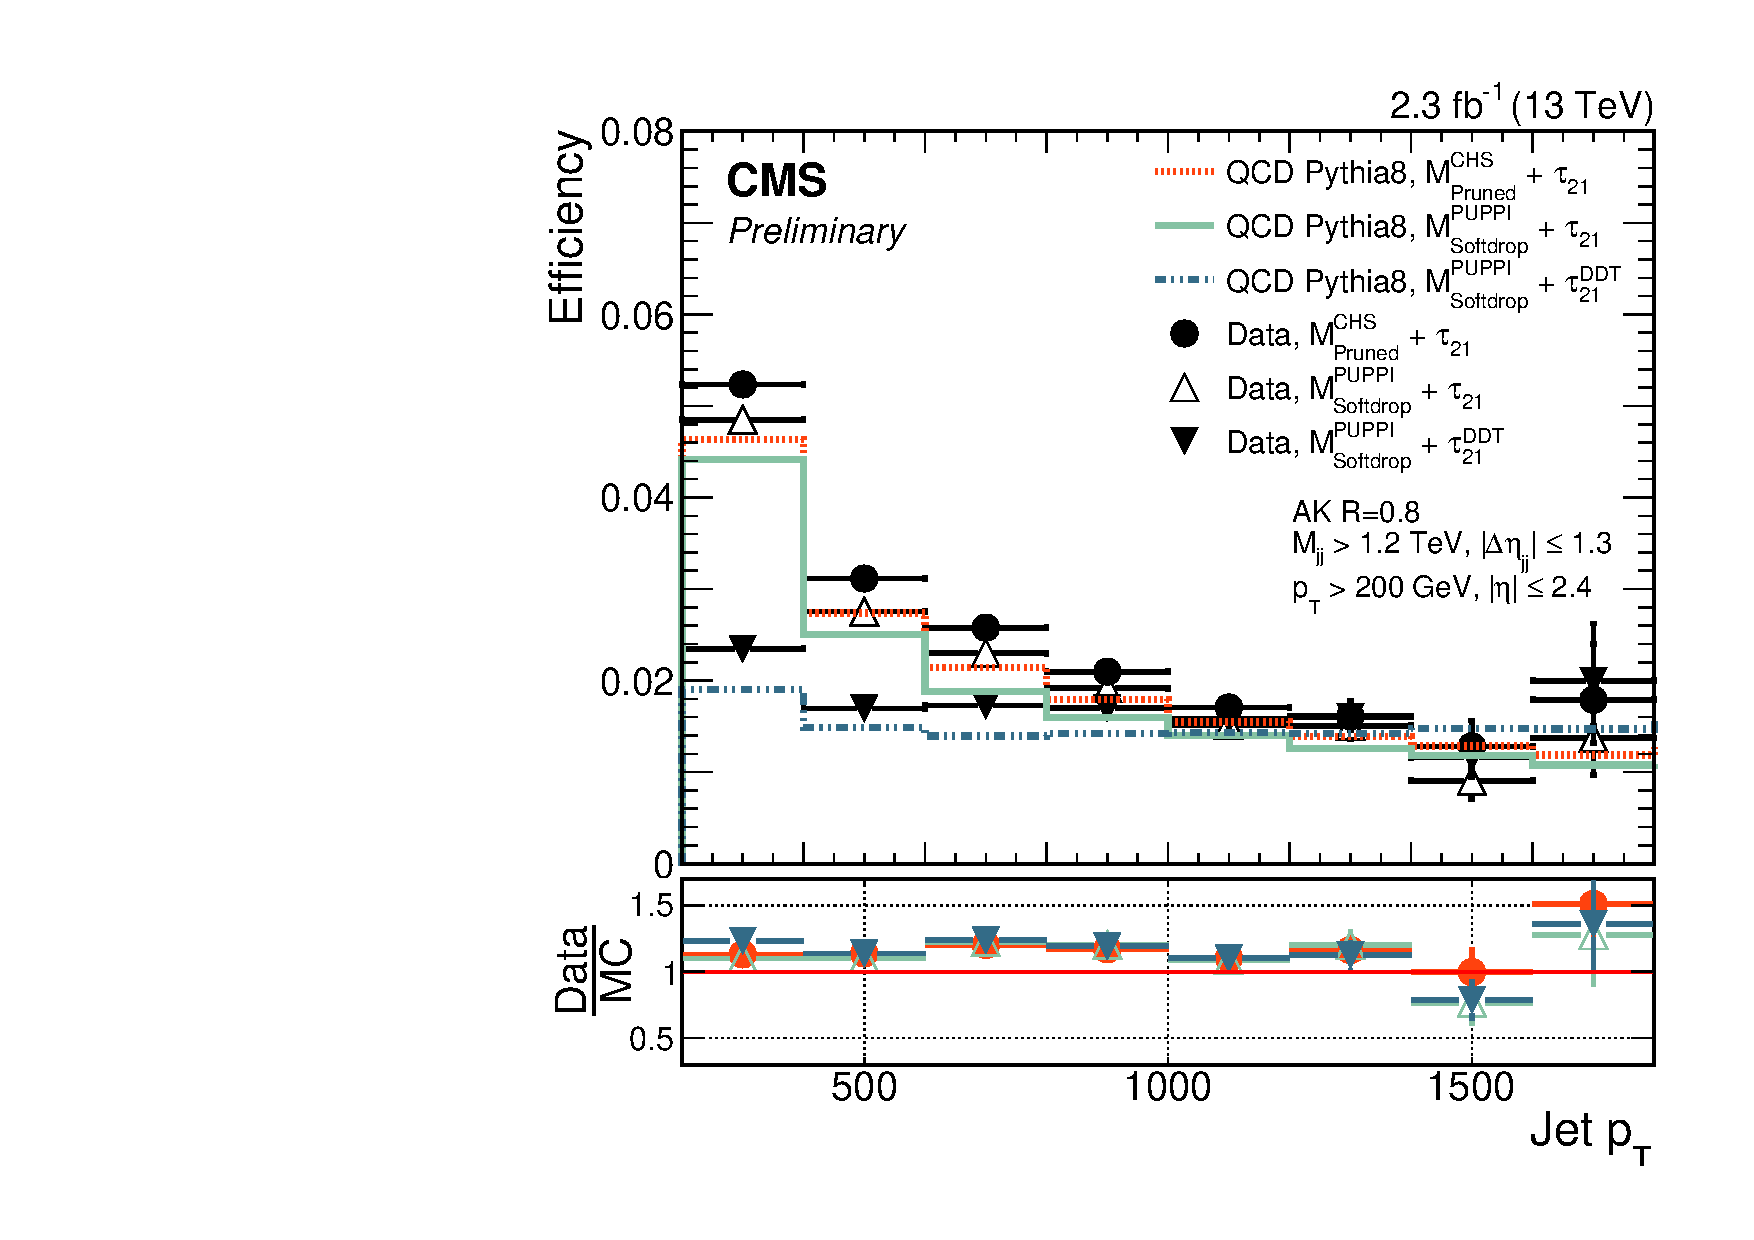
\includegraphics[width=0.49\textwidth]{figures/vtagging/JME-16-003/BoostedW/BkgEff_DataMC_Pythia8_pT.pdf}\\
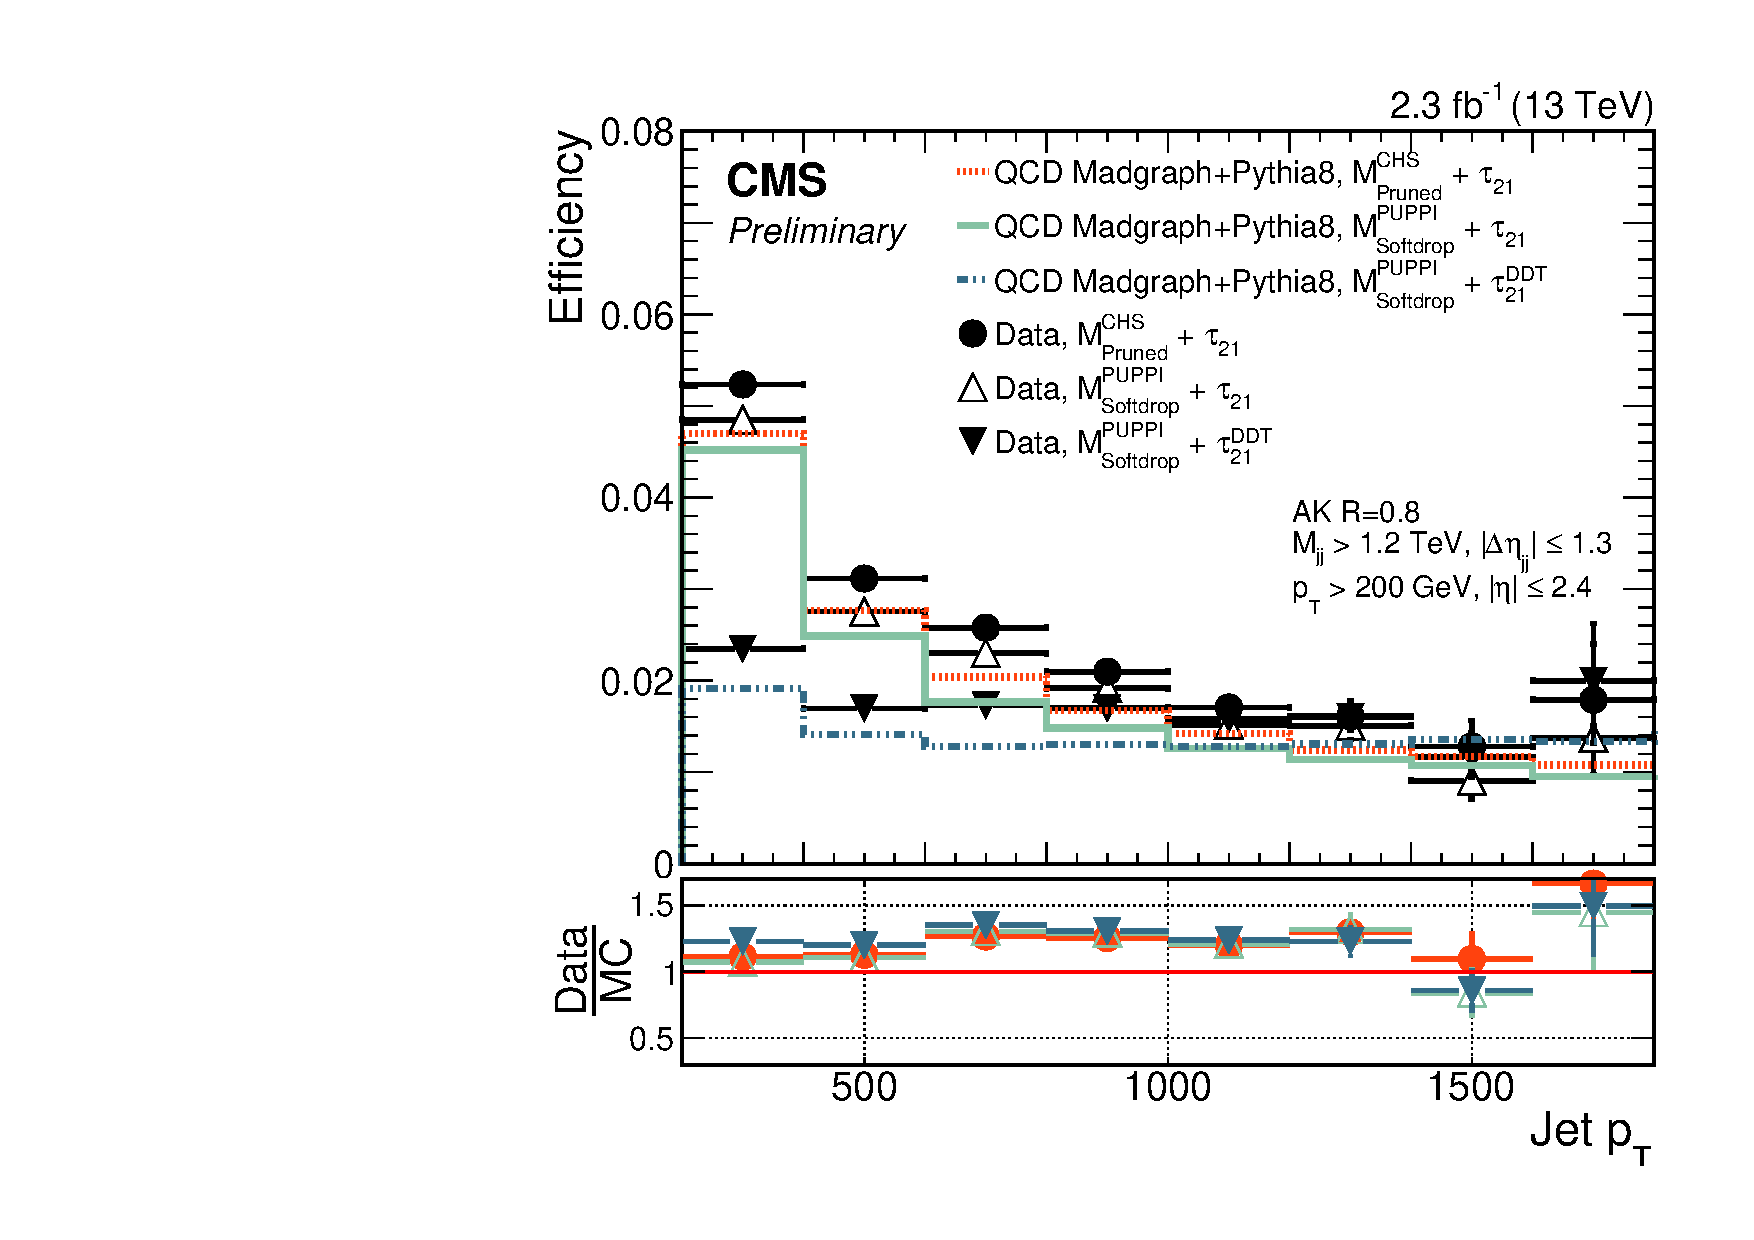
\includegraphics[width=0.49\textwidth]{figures/vtagging/JME-16-003/BoostedW/BkgEff_DataMC_Pythia8Madgraph_pT.pdf}
\caption{ 
The fraction of jets that pass the $m_{\mathrm{jet}}$ + $\tau_2/\tau_1$ selections in a dijet enriched sample for data and for simulation as a function of jet \PT. Here comparing \HERWIG{++} (left), \PYTHIA{8} (right) and \PYTHIA{8} with \MADGRAPH as matrix-element generator (left).}
\label{fig:searchII:fakerate}
\end{figure}
We find a substantial difference in the modeling of substructure variables between the different generators, most likely coming from their very different description of gluon radiation (dominant in QCD multijet events).
The best description is obtained with \HERWIG{++}, while all three generators model the tagging \PT dependence well.
We additionally study the difference in the total quark/gluon-content for the two PUPPI softdrop based taggers: \nsubj and \ddt. Figure~\ref{fig:searchII:qgfakerate} shows the stacked relative q/g content in a Pythia 8 QCD dijet sample for a cut on PUPPI \nsubj and \ddt. We see that the quark content increases as a function of jet \PT when cutting on the DDT, while it decreases when cutting on \nsubj.
\begin{figure}[htbp]
\centering
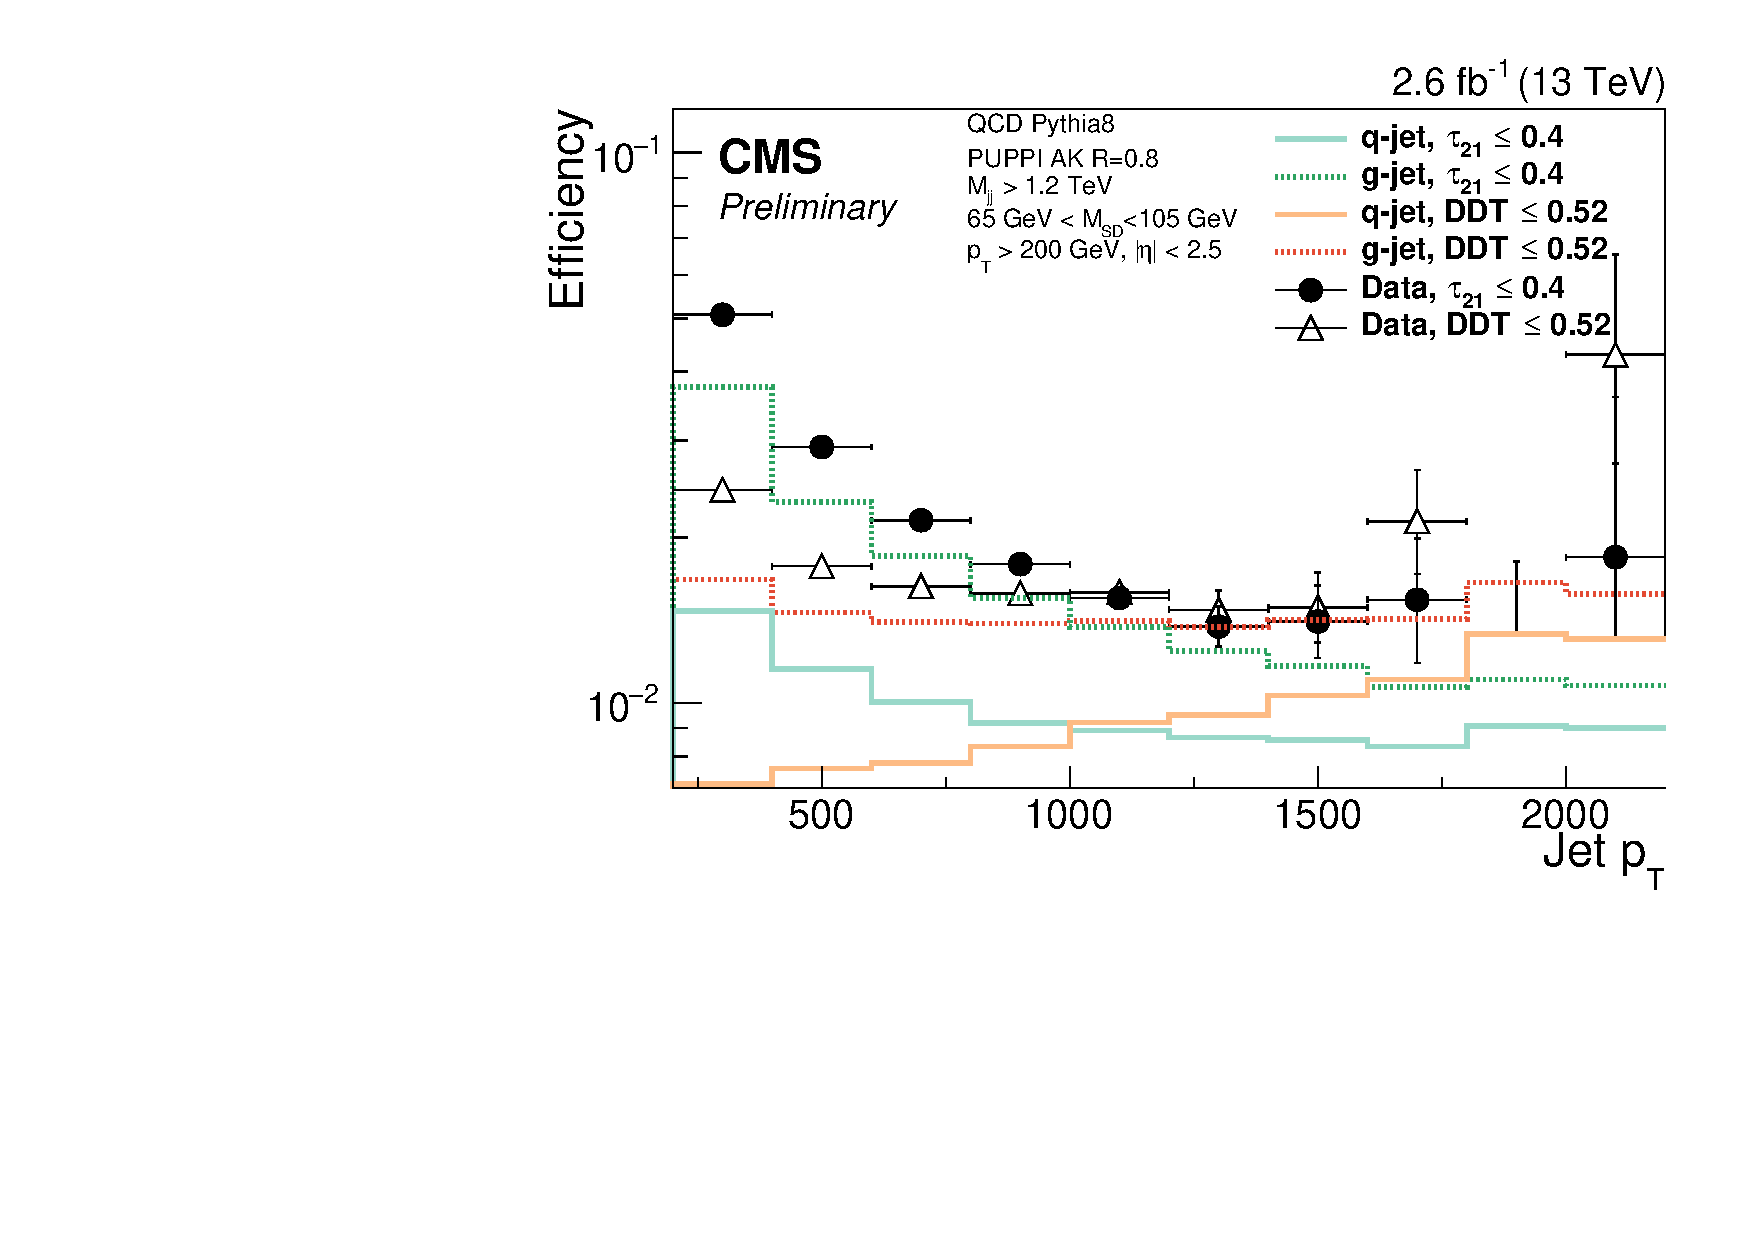
\includegraphics[width=0.49\textwidth]{figures/vtagging/JME-16-003/BoostedW/qgFakeRate_Pythia8_pT.pdf}
\caption{ 
The fraction of jets that pass the PUPPI softdrop $m_{\mathrm{jet}}$ with $\tau_2/\tau_1$ (turquoise) or \ddt (orange) selections in a dijet enriched sample. The jets from QCD MC are split into two contributions: jets originating from gluons (dotted line) and jets originating from quarks (solid line).}
\label{fig:searchII:qgfakerate}
\end{figure}
 This can be attributed to the fact that the $m/\PT$ distribution for quark and gluon jets are very different from one another, and this difference increase as the jet \PT increases. Figure~\ref{fig:searchII:mpt_qvsg} shows the $m/\PT$ for jets originating from a quark (blue) and a gluon (red) for a jet \PT of 200 \GeV (left) and 1600 \GeV. We see that the mass over \PT for gluon jets is significantly higher for gluon jets than for quark jets.
 With the \ddt tagger being defined as in Equation~\ref{eq:searchII:ddt}, the DDT will therefore act more aggressive on jets with a high $m/\PT$, effectively removing more gluon jets.
\begin{figure}[ht!]
\centering
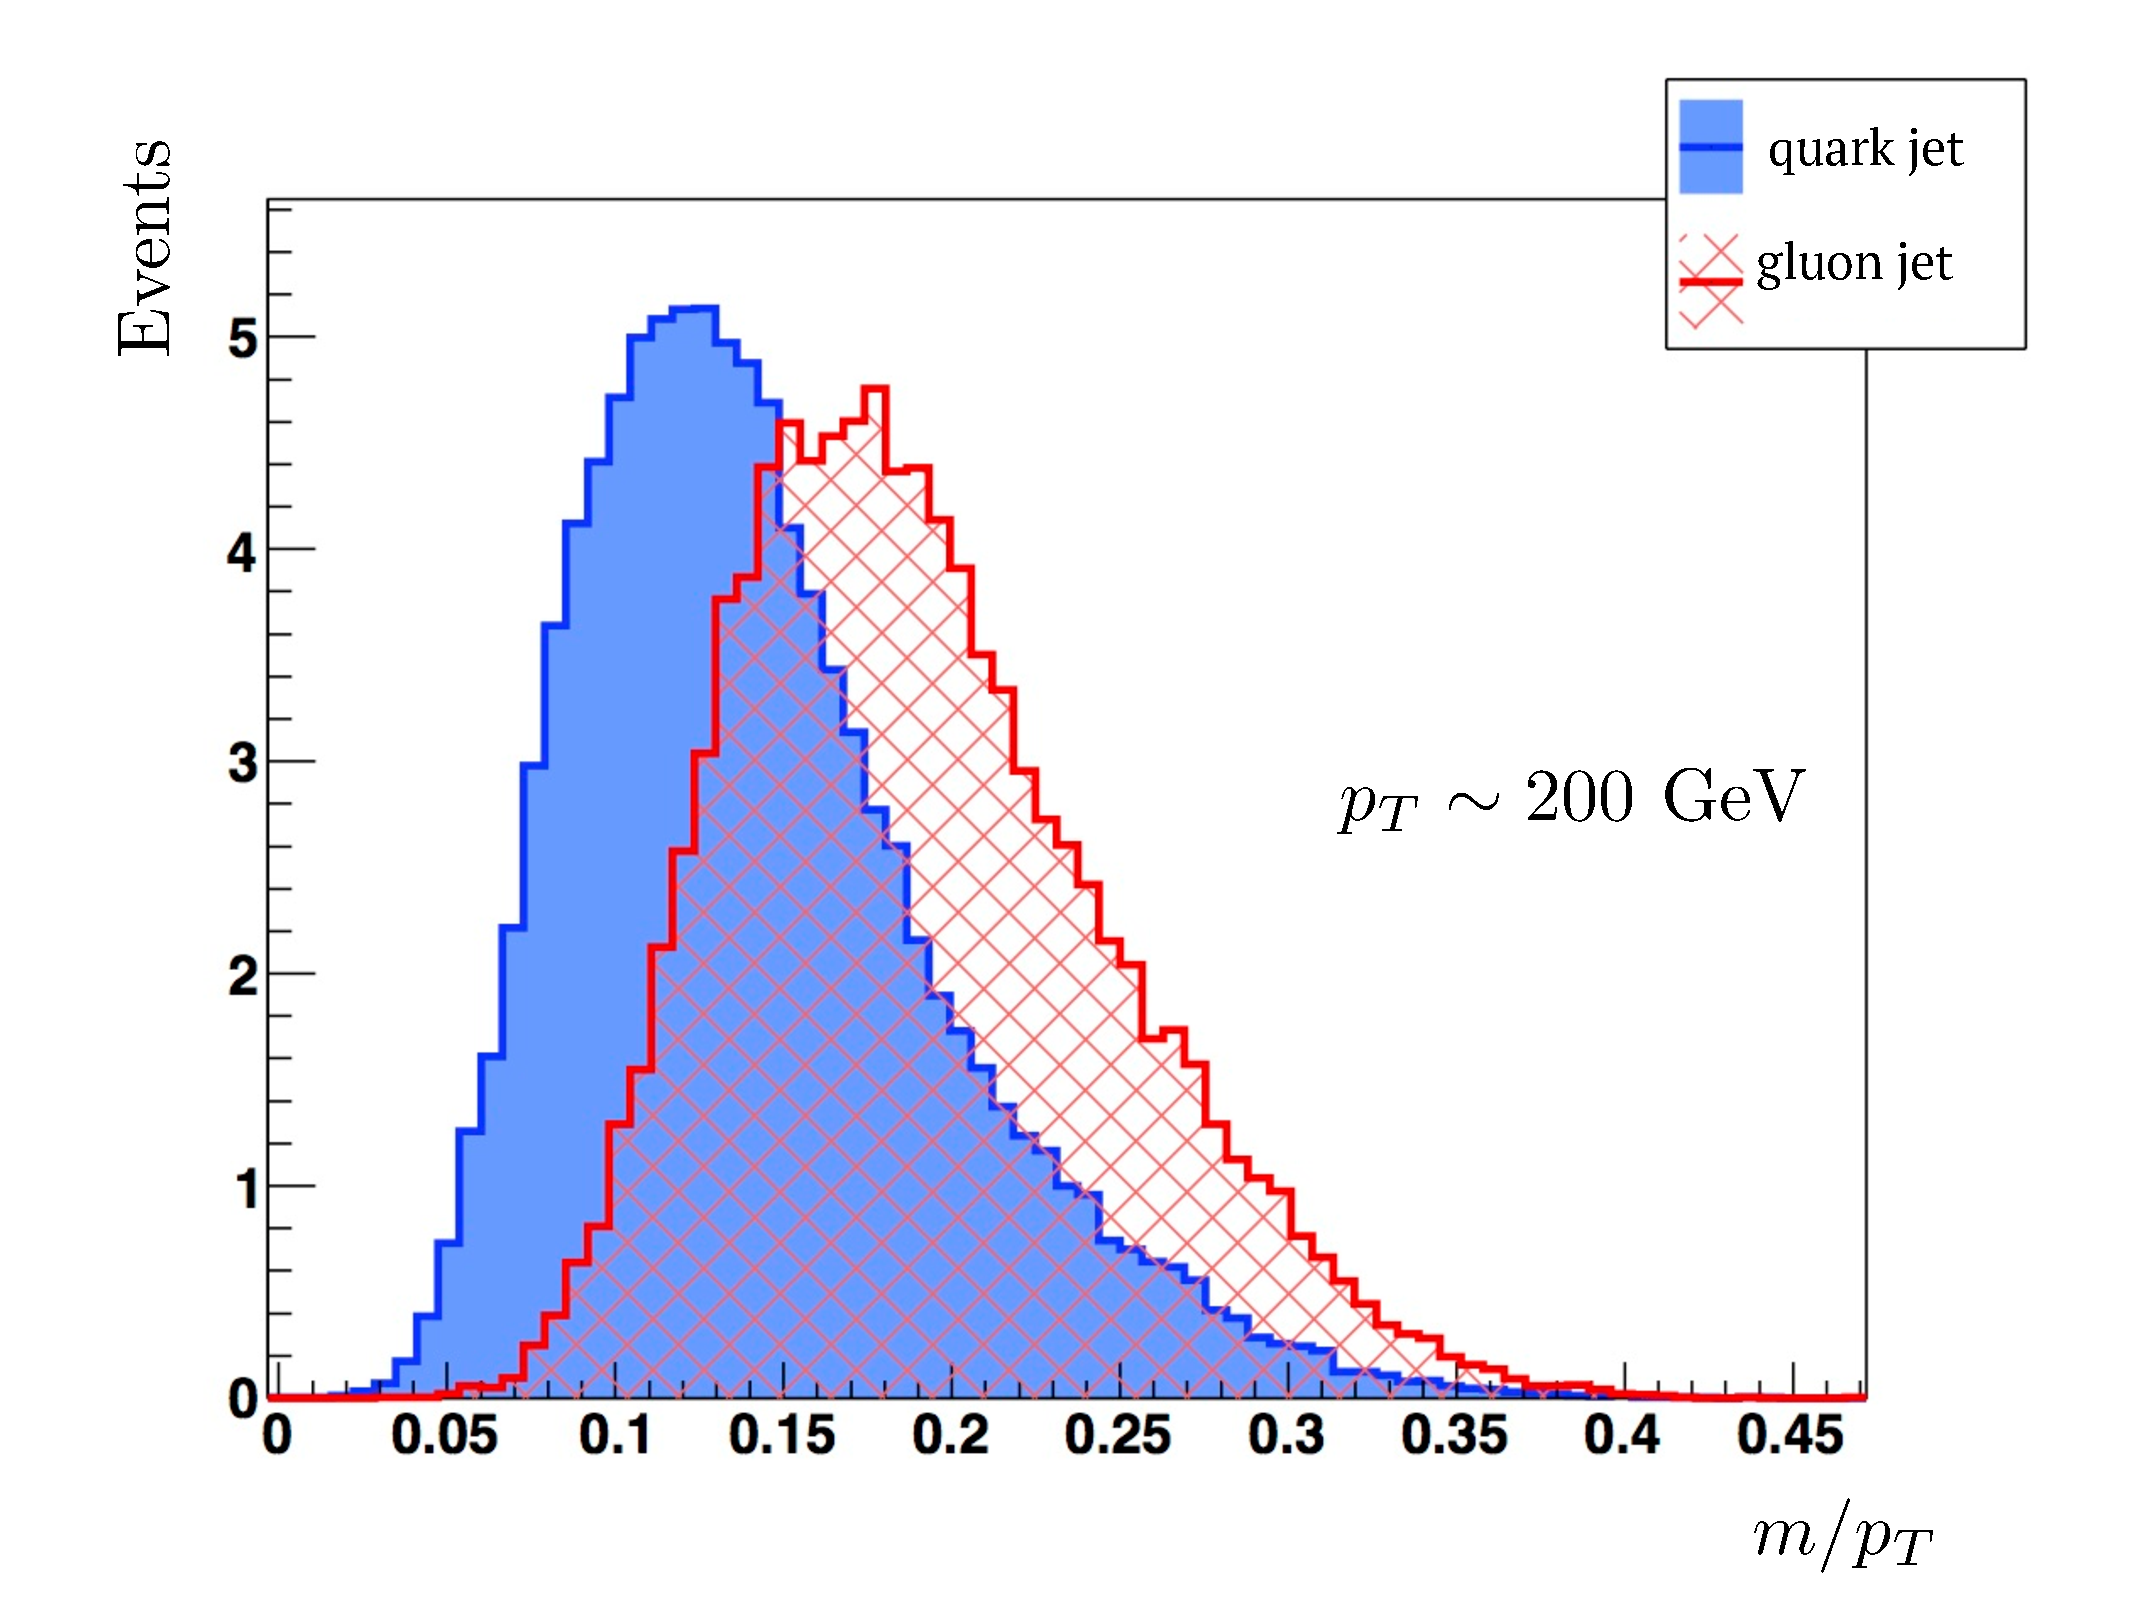
\includegraphics[width=0.49\textwidth]{figures/analysis/search2/misc/ak07_MDPt_0200.pdf}
\includegraphics[width=0.49\textwidth]{figures/analysis/search2/misc/ak07_MDPt_1600.pdf}
\caption{The jet mass divided by the jet \PT for quark(blue) and gluon (red) jets for a jet \PT of 200 (left) and 1600 \GeV (right). Created with~\cite{Gallicchio:2011xq}.}
\label{fig:searchII:mpt_qvsg}
\end{figure}
\clearpage

\subsection{Mass and purity categorization}
The PUPPI softdrop jet mass and PUPPI \nsubj distribution after loose analysis preselections, as outlined in Section~\ref{sec:searchII:samples}, are shown in Figure~\ref{fig:searchII:wtag}.
We see some disagreement between data and MC, especially in the high-purity region (PUPPI $\ddt<0.4$), confirming what we observed in Section~\ref{sec:searchII:wmistag}
\begin{figure}[h!]
\centering
\includegraphics[width=0.49\textwidth]{figures/analysis/search2/AN-16-235/plots/qcdcp_PuppiSoftdropMass.pdf}
\includegraphics[width=0.49\textwidth]{figures/analysis/search2/AN-16-235/plots/qcdcp_puppi_tau2tau1.pdf}
\caption{PUPPI softdrop jet mass distribution (left) and PUPPI n-subjettiness $\tau_{21}$ (right) distribution for data and simulated samples. Simulated samples are scaled to match the distribution in data.}
\label{fig:searchII:wtag}
\end{figure}
As this analysis is sensitive to both heavy resonances decaying into two vector bosons and excited quark resonances $q^*$ decaying to qW and qZ, we look for events with both a single W/Z-tag and events with two W/Z-tags. 
Vector boson candidates are selected with a PUPPI softdrop jet mass of $65<m_{\mathrm{jet}}<105$~\GeV. Further, and similar to what was done in Search I, we select "high purity" (HP) W/Z jets by requiring  PUPPI $0<\tau_{21} \leq 0.40$ and "low purity" (LP) jets with $0.40<\tau_{21}\leq0.75$. The events with one W/Z-tag are classified in HP and LP events according to the two categories described previously. Events with two W/Z-tagged jets are always required to have one HP tagged jet, and are further divided into LP and HP categories depending on whether the other jet is of high or low purity. We additionally split into two mass categories in order to enhance the analysis sensitivity, with the W window defined as $65 {\GeV} < m_{pruned} < 85 {\GeV}$ and the Z boson window as $85 {\GeV} < m_{pruned} < 105 {\GeV}$. This results in ten different signal categories. They are as follows:
\begin{itemize}
\item High-purity double W/Z-tag, 3 mass categories: WW, ZZ and WZ
\item Low-purity double W/Z-tag, 3 mass categories: WW, ZZ and WZ
\item High-purity single W/Z-tag, 2 mass categories: qW and qZ
\item Low-purity single W/Z-tag, 2 mass categories: qW and qZ
\end{itemize}

\subsection{Background modeling: F-test} 
\label{sec:searchII:ftest}
With the full analysis selections and categorization defined, we move to the determination of background fit function. Following the same strategy as in Section~\ref{sec:searchI:bkg}, we determine the number of necessary parameters in order to describe the background through a Fishers F-test, comparing the same fit functions as in Section~\ref{sec:searchI:bkg}. This test is first exercised in QCD MC and then in a data sideband before the final determination in the data signal region. As the F-test results were presented in detail in the context of Search I, only a brief summary and the fits in the new single-tag categories will be presented here, while all fits and F-test results can be found in Appendix~\ref{app:2016xcheck}.\newline
A two or three parameter fit is sufficient to describe the background for all the double tag categories: a two parameter fit is sufficient for the "high-purity" WZ and ZZ categories. 
as well as the "low-purity" WW category, while the remaining analysis categories require a three parameter background fit.
From the fits to the single tag categories, shown in Figure~\ref{fig:searchII:bkgfit_sr_qv}, a three parameter fit is sufficient for all categories except the "high-purity" qW category. In this category the improvement in fit quality when increasing the number
of parameters is so large adding that adding an additional fit parameter is justified, and we continue by using a 5 parameter fit for this category. 
\begin{figure}[h!]
\centering
\includegraphics[width=0.45\textwidth]{figures/analysis/search2/AN-16-235/plots/qWHP.pdf}
\includegraphics[width=0.45\textwidth]{figures/analysis/search2/AN-16-235/plots/qWLP.pdf}\\
\includegraphics[width=0.45\textwidth]{figures/analysis/search2/AN-16-235/plots/qZHP.pdf}
\includegraphics[width=0.45\textwidth]{figures/analysis/search2/AN-16-235/plots/qZLP.pdf}\\
\caption{Background fit for the $M_{jj}$ distribution in the data signal region for the single-tag analysis. Here for the high- (left) and low-purity (right) single W/Z-tag categories qW (top) and qZ (bottom).}
\label{fig:searchII:bkgfit_sr_qv}
\end{figure}
A summary of what fit functions are used for each analysis category is listen in Table~\ref{tab:searchII:fitpars}.
\begin{table}[htb]
\centering
\begin{tabular}{|l| c | c|}
\hline
Mass category & \multicolumn{2}{|c|}{N pars.}\\
\hline
& HP & LP \\
\hline
WW & 3 & 2 \\
WZ & 2 & 3 \\
ZZ & 2 & 3 \\
qW & 5 & 3 \\
qZ & 3 & 3 \\
\hline
\end{tabular}
\caption{Fit parameters used in each analysis category}
\label{tab:searchII:fitpars}
\end{table}

\subsection{Signal modeling}
The signal is modeled from signal MC in the same way as was done in Section~\ref{sec:searchI:sig}, assuming a Gaussian core and an exponential tail. The interpolated signal shapes for $\rm{q}^* \rightarrow \rm{q}\PW$ and $\rm{q}^* \rightarrow \rm{q}\PZ$ in their most sensitive analysis categories ($\rm{q}\PW$ and $\rm{q}\PZ$,respectively) are shown in Figure \ref{fig:searchII:interpolation}. The signal shapes for the double-tag category can be compared to those in Figure~\ref{fig:searchI:sigfit}.
 
\begin{figure}[htbp]
\centering
\includegraphics[width=0.49\textwidth]{figures/analysis/search2/AN-16-235/plots/interpolation_QstarQZ_DijetMassHighPuriqZ.pdf}
\includegraphics[width=0.49\textwidth]{figures/analysis/search2/AN-16-235/plots/interpolation_QstarQW_DijetMassHighPuriqW.pdf}\\
\caption{Interpolated signal shapes for a  $q*\rightarrow qZ$ (left) and $q*\rightarrow qW$ (right) signal.}
\label{fig:searchII:interpolation}
\end{figure}


\subsection{Systematic uncertainties}
The largest sources of systematic uncertainty for this analysis is, as for Search I, related to the signal modeling and are due to the uncertainty in the tagging efficiency of the W/Z-tagger, the jet energy/mass scale, the jet energy/mass resolution and integrated luminosity. The W/Z tagging uncertainty is estimated in $\rm{t\bar{t}}$ events, as described in Section~\ref{sec:searchI:vtag}, and yield uncertainties on the scale factors for the HP and LP tagging categories.
The \pt- and $\eta$-dependent jet energy scale and resolution uncertainties on the resonance shape were approximated by a constant 2\% and 10\% uncertainty in Search I (Section~\ref{sec:searchI:wtagsystematic}) and are not expected to change for the 2016 analysis. The jet energy response and resolution uncertainty are taken into account as shape uncertainty by shifting and widening the signal resonance model,
while all other signal uncertainties only affect the yield. The list of most relevant systematic uncertainties are listed in Table~\ref{tab:searchII:VV_systematicssummary_signal}.
\begin{table}[htb]
  \centering
  \begin{tabular}{lccc}
    \hline
    Source                        & Relevant quantity      & HP+HP unc. (\%)  & HP+LP unc. (\%)\\
    \hline
    Jet energy scale                 & Resonance shape        & 2                    & 2 \\
    Jet energy resolution            & Resonance shape        & 10                   & 10 \\
    \hline
    Jet energy scale                 & Signal yield           & \multicolumn{2}{c}{$<$0.1--4.4}\\ 
    Jet energy resolution            & Signal yield           & \multicolumn{2}{c}{$<$0.1--1.1}\\
    Jet mass scale                   & Signal yield           & \multicolumn{2}{c}{0.02--1.5}\\ 
    Jet mass resolution              & Signal yield           & \multicolumn{2}{c}{1.3--6.8}\\ 
    Pileup                           & Signal yield           & \multicolumn{2}{c}{2}\\
    Integrated luminosity            & Signal yield           & \multicolumn{2}{c}{6.2}\\
    PDFs (\PWpr)                     & Signal yield		       & \multicolumn{2}{c}{4--19}\\
    PDFs (\PZpr)                     & Signal yield		       & \multicolumn{2}{c}{4--13}\\
    PDFs (\BulkG)                    & Signal yield		       & \multicolumn{2}{c}{9--77}\\
    Scales (\PWpr)                   & Signal yield		       & \multicolumn{2}{c}{1--14}\\
    Scales (\PZpr)                   & Signal yield		       & \multicolumn{2}{c}{1--13}\\
    Scales (\BulkG)                  & Signal yield		       & \multicolumn{2}{c}{8--22}\\
    \hline
    % Jet energy scale                 & Migration              & \multicolumn{2}{c}{0--14}\\
%     Jet energy resolution            & Migration              & \multicolumn{2}{c}{0--4.1}\\
    Jet mass scale                   & Migration              & \multicolumn{2}{c}{$<$0.1--16.8}\\
    Jet mass resolution              & Migration              & \multicolumn{2}{c}{$<$0.1--17.8}\\
    W-tagging \nsubj{}               & Migration              & 15.6                  & 21.9\\
    W-tagging \pt-dependence         & Migration              & 7--14                 & 5--11\\
    \hline
  \end{tabular}
  \caption{Summary of the signal systematic uncertainties for the analysis and their impact on the event yield in the signal region and on the reconstructed dijet invariant mass shape (mean and width).}
  \label{tab:searchII:VV_systematicssummary_signal}
\end{table}

\subsection{Results}   
As mentioned in the introduction to this chapter, the analysis of the 2016 dataset was done in two steps: One based on 12.9 \fbinv of early 2016 data, demonstrating the new PUPPI softdrop based tagger and single-tag analysis categories, and one topping up with the full 35.9 \fbinv dataset. The results from both will be presented in the following.

\subsubsection{Early analysis}   
\label{sec:searchII:b2g16021res}
Exclusion limits are set in the context of the bulk graviton model, the HVT model~B scenario and excited quark resonances,
assuming the resonances to have a natural width negligible with respect to the experimental resolution (as in Search I).

Figure~\ref{fig:searchII:limitCombined} shows the 95\% confidence level (CL) expected and observed exclusion limits on the signal cross section as a function of the resonance mass for the different signal hypotheses in the double-tag analysis.
The limits are compared with the cross section times the branching fraction to $\PW\PW$ and $\PZ\PZ$ for a bulk graviton with $\ktilde = 0.5$, and with the cross section
times the branching fraction to $\PW\PZ$ and $\PW\PW$ for spin-1 particles predicted by the HVT model~B for both the singlet (\PWpr or \PZpr) and triplet (\PWpr and \PZpr) hypothesis.
For the HVT model B, we exclude \PWpr(\PZpr) resonances with masses below 2.7 (2.6)~\TeV. The signal cross section uncertainties are displayed as a red checked band and result in an additional uncertainty on the resonance mass limits of 0.05 (0.04)~\TeV.
The cross section limits for $\PZpr \rightarrow \PW\PW$ and $\rm G_{bulk}\rightarrow\PW\PW$ are not identical due to the different acceptance for those two signal scenarios.

\begin{figure}[htbp]
\centering
     \includegraphics[width=0.45\textwidth]{figures/analysis/search2/B2G-16-021/figures/limits/brazilianFlag_ZprimeWW_new_combined_13TeV.pdf}
     \includegraphics[width=0.45\textwidth]{figures/analysis/search2/B2G-16-021/figures/limits/brazilianFlag_WZ_new_combined_13TeV.pdf}\\
     \includegraphics[width=0.45\textwidth]{figures/analysis/search2/B2G-16-021/figures/limits/brazilianFlag_BulkWW_new_combined_13TeV.pdf}
     \includegraphics[width=0.45\textwidth]{figures/analysis/search2/B2G-16-021/figures/limits/brazilianFlag_BulkZZ_new_combined_13TeV.pdf}
\caption{Observed (black solid) and expected (black dashed) 95\% CL upper limits on the production of a narrow-width resonance decaying to a pair of vector bosons for different signal hypotheses. 
Limits are set in the context of a spin-1 neutral \PZpr (left) and charged \PWpr (right) resonances resonance, and compared with the prediction of the HVT model~B. On the bottom, limits are set in the context of a bulk graviton decaying into $\PW\PW$ (left) and $\PZ\PZ$ (right) with $\ktilde =0.5$ and compared with the model prediction. Signal cross section uncertainties are displayed as a red checked band.
}
\label{fig:searchII:limitCombined}
\end{figure}

Figure~\ref{fig:limitCombined_qV} shows the corresponding exclusion limits for excited quarks decaying into q\PW and q\PZ.
We exclude excited quark resonances decaying into q\PW and q\PZ with masses below 5.0 and 3.9~\TeV, respectively.
The signal cross section uncertainties are displayed as a red checked band and result in an additional uncertainty on the resonance mass limits of 0.1~\TeV.

\begin{figure}[htbp]
\centering
     \includegraphics[width=0.45\textwidth]{figures/analysis/search2/B2G-16-021/figures/limits/brazilianFlag_qW_new_combined_13TeV.pdf}
     \includegraphics[width=0.45\textwidth]{figures/analysis/search2/B2G-16-021/figures/limits/brazilianFlag_qZ_new_combined_13TeV.pdf}\\
\caption{Observed (black solid) and expected (black dashed) 95\% CL upper limits on the production of an excited quark resonance
decaying into qW (left) or qZ (right). Signal cross section uncertainties are displayed as a red checked band.
}
\label{fig:searchII:limitCombined_qV}
\end{figure}



\subsubsection{Full 2016 dataset}   
\label{sec:searchII:brg17001res}

The results obtained with the full $\sim 36$ \fbinv of 2016 data are as follows:
For a \BulkG we exclude production cross sections in a range from 36.0~fb, at a resonance mass of 1.3\TeV, to 0.6~fb at resonance masses above 3.6\TeV. \PWpr(\PZpr) resonances are excluded with masses below 3.2 (2.7)\TeV for the HVT model B, in addition to \PWpr resonances with a mass between 3.3 and 3.6 \TeV. For excited quark resonances, we can exclude the production of $\rm{q}^*$ decaying to qW or qZ for masses below 5.0 and 4.7 TeV.
Figure~\ref{fig:searchII:limitCombined_VV} and~\ref{fig:searchII:limitCombined_qV} show the resulting 95\% confidence level expected and observed exclusion limits on the signal cross section as a function of the resonance mass for VV and QV resonances, respectively.

\begin{figure}[h!]
\centering
    \includegraphics[width=0.49\textwidth]{figures/analysis/search2/B2G-17-001/figures/brazilianFlag_BulkWW_VVnew_new_combined_13TeV.pdf}
    \includegraphics[width=0.49\textwidth]{figures/analysis/search2/B2G-17-001/figures/brazilianFlag_WZ_VVnew_new_combined_13TeV.pdf}\\
    \includegraphics[width=0.49\textwidth]{figures/analysis/search2/B2G-17-001/figures/brazilianFlag_BulkZZ_VVnew_new_combined_13TeV.pdf}
\caption{Observed (solid line) and expected (dashed line) 95\% CL upper limits on the production cross section of a narrow resonance decaying into two vector bosons for different signal hypotheses: A \PZpr or \BulkG resonance decaying into \WW (top left), a \PZpr decaying into \PW\PZ (top right) and a bulk graviton decaying into \ZZ (bottom).}
\label{fig:searchII:limitCombined_VV}
\end{figure}

\begin{figure}[ht!]
\centering
    \includegraphics[width=0.49\textwidth]{figures/analysis/search2/B2G-17-001/figures/brazilianFlag_qW_qVnew_new_combined_13TeV.pdf}
    \includegraphics[width=0.49\textwidth]{figures/analysis/search2/B2G-17-001/figures/brazilianFlag_qZ_qVnew_new_combined_13TeV.pdf}\\
\caption{Observed (solid line) and expected (dashed line) 95\% CL upper limits on the production of an excited quark resonance
decaying into qW (left) or qZ (right).}
\label{fig:searchII:limitCombined_qV}
\end{figure}


